\documentclass[italian,12pt,a4paper,oneside,final]{report}
\usepackage[toc]{appendix}
\usepackage{listings}
\usepackage{graphicx}
\usepackage{subcaption}
\usepackage[utf8]{inputenc}
\usepackage[T1]{fontenc}
\usepackage[backend=biber,style=numeric,sorting=none]{biblatex} %Imports biblatex package
\addbibresource{cnn2.bib} %Import the bibliography file
\usepackage[italian]{babel}
\usepackage[style=italian/quotes]{csquotes}
\usepackage{hyperref}
\graphicspath{ {images/} }
\lstset{
	captionpos=b,
	showspaces=false,
	basicstyle=\ttfamily,
	showstringspaces=false,
	breaklines=true,
	frame=line,
}
\renewcommand{\thesection}{\arabic{section}} % remove the \chapter counter from being printed with every \section
\renewcommand{\appendixtocname}{Appendice}
\renewcommand{\appendixpagename}{Appendice}
\hypersetup{
	colorlinks=true,
	citecolor=,
	linkcolor=,
	urlcolor=blue,
	pdftitle={Marco Giunta - Progetto ML},
	pdfauthor={Marco Giunta},
}


\title{\Large CNN2: Viewpoint Generalization via a Binocular Vision\\[0.5em]
\large Reproducibility Challenge}
\date{Luglio 2025}
\author{
Marco Giunta\thanks{Marco Giunta 147852 giunta.marco@spes.uniud.it}}


\begin{document}
\pagenumbering{roman}% To avoid duplicate hyperref links to pages with same page number
% Generate title page
\maketitle

% Generate TOCs
\pagenumbering{arabic}
\tableofcontents

\newpage
\section{Introduzione}

Lo scopo di questo progetto è riprodurre i risultati dell'articolo \citetitle{neurips2019:cnn2}\cite{neurips2019:cnn2} come proposto nella \citetitle{neurips2019:reproducibility-challenge}\cite{neurips2019:reproducibility-challenge}.
In particolare, l'obiettivo è quello di replicare i risultati principali presentati nell'articolo, senza utilizzare il codice rilasciato dagli autori, leggendo solo l'articolo e i materiali supplementari.

Il modello realizzato in questo progetto è stato creato da zero usando la libreria PyTorch (versione 2.5.1) e testato su una workstation con CPU Intel\textsuperscript{\tiny{\textregistered}} Xeon\textsuperscript{\tiny{\textregistered}} E5620, 128GB RAM e una GPU NVIDIA GeForce GTX 1080 Ti (driver Nvidia 550.90.07 e CUDA Toolkit 12.1 Update 1).

\subsection{Articolo originale}
Nell'articolo originale gli autori propongono il modello CNN\textsuperscript{2}, una rete neurale convoluzionale che riceve in input due immagini binoculari di un oggetto ed è in grado di riconoscere quell'oggetto da angolazioni diverse da quelle usate per l'addestramento del modello.

\subsubsection{Modello}
In figura~\ref{fig:cnn2_model} possiamo vedere l'architettura del modello CNN\textsuperscript{2}.
\begin{figure}[ht]
	\centering
	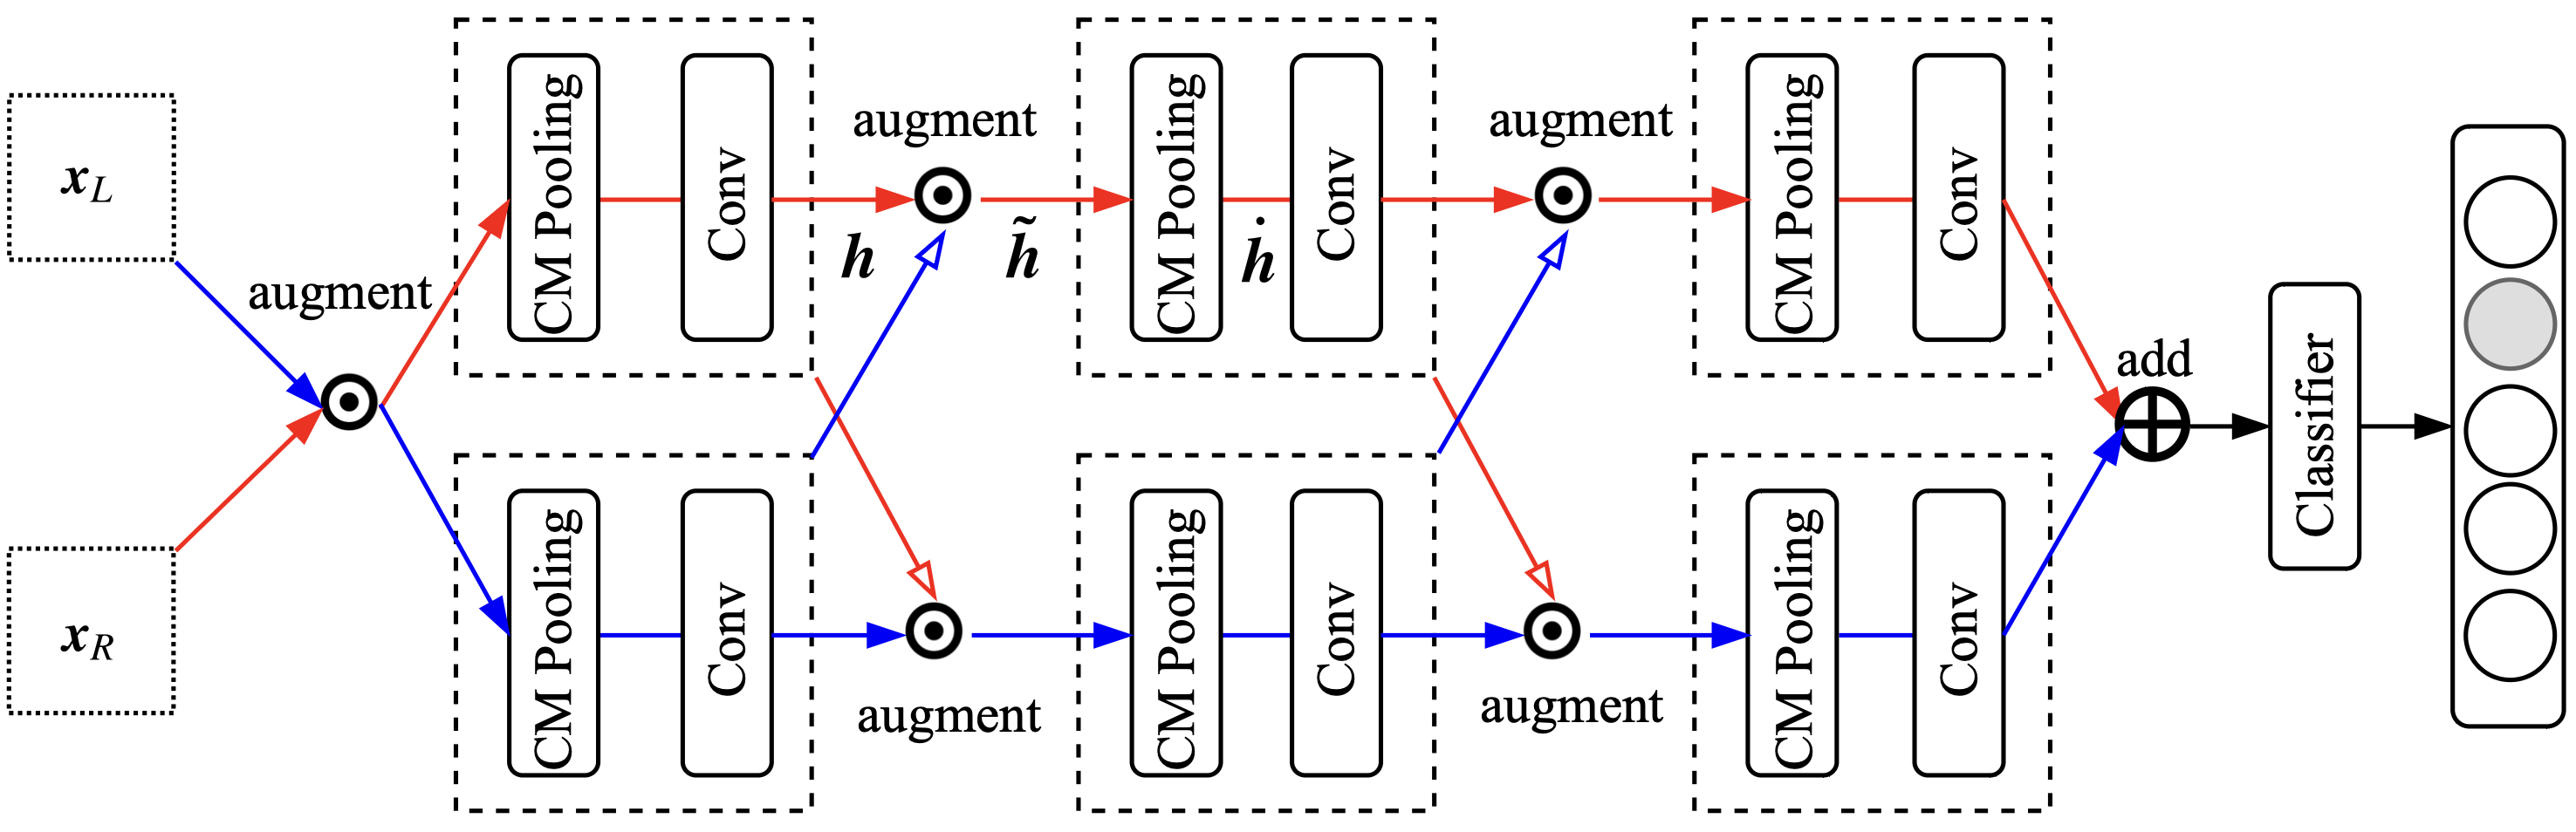
\includegraphics[width=0.8\textwidth]{model-cnn2.png}
	\caption{Modello CNN2}
	\label{fig:cnn2_model}
\end{figure}
A differenza di una CNN tradizionale, questo modello usa per le immagini dell'occhio sinistro e destro due percorsi di \textit{feedforward} paralleli ma complementari.
A ogni \textit{layer}, le immagini binoculari vengono combinate e poi suddivise seguendo la procedura di \textit{parallax augmentation} visibile in figura~\ref{fig:cnn2_parallax}.

\begin{figure}[!ht]
	\centering
	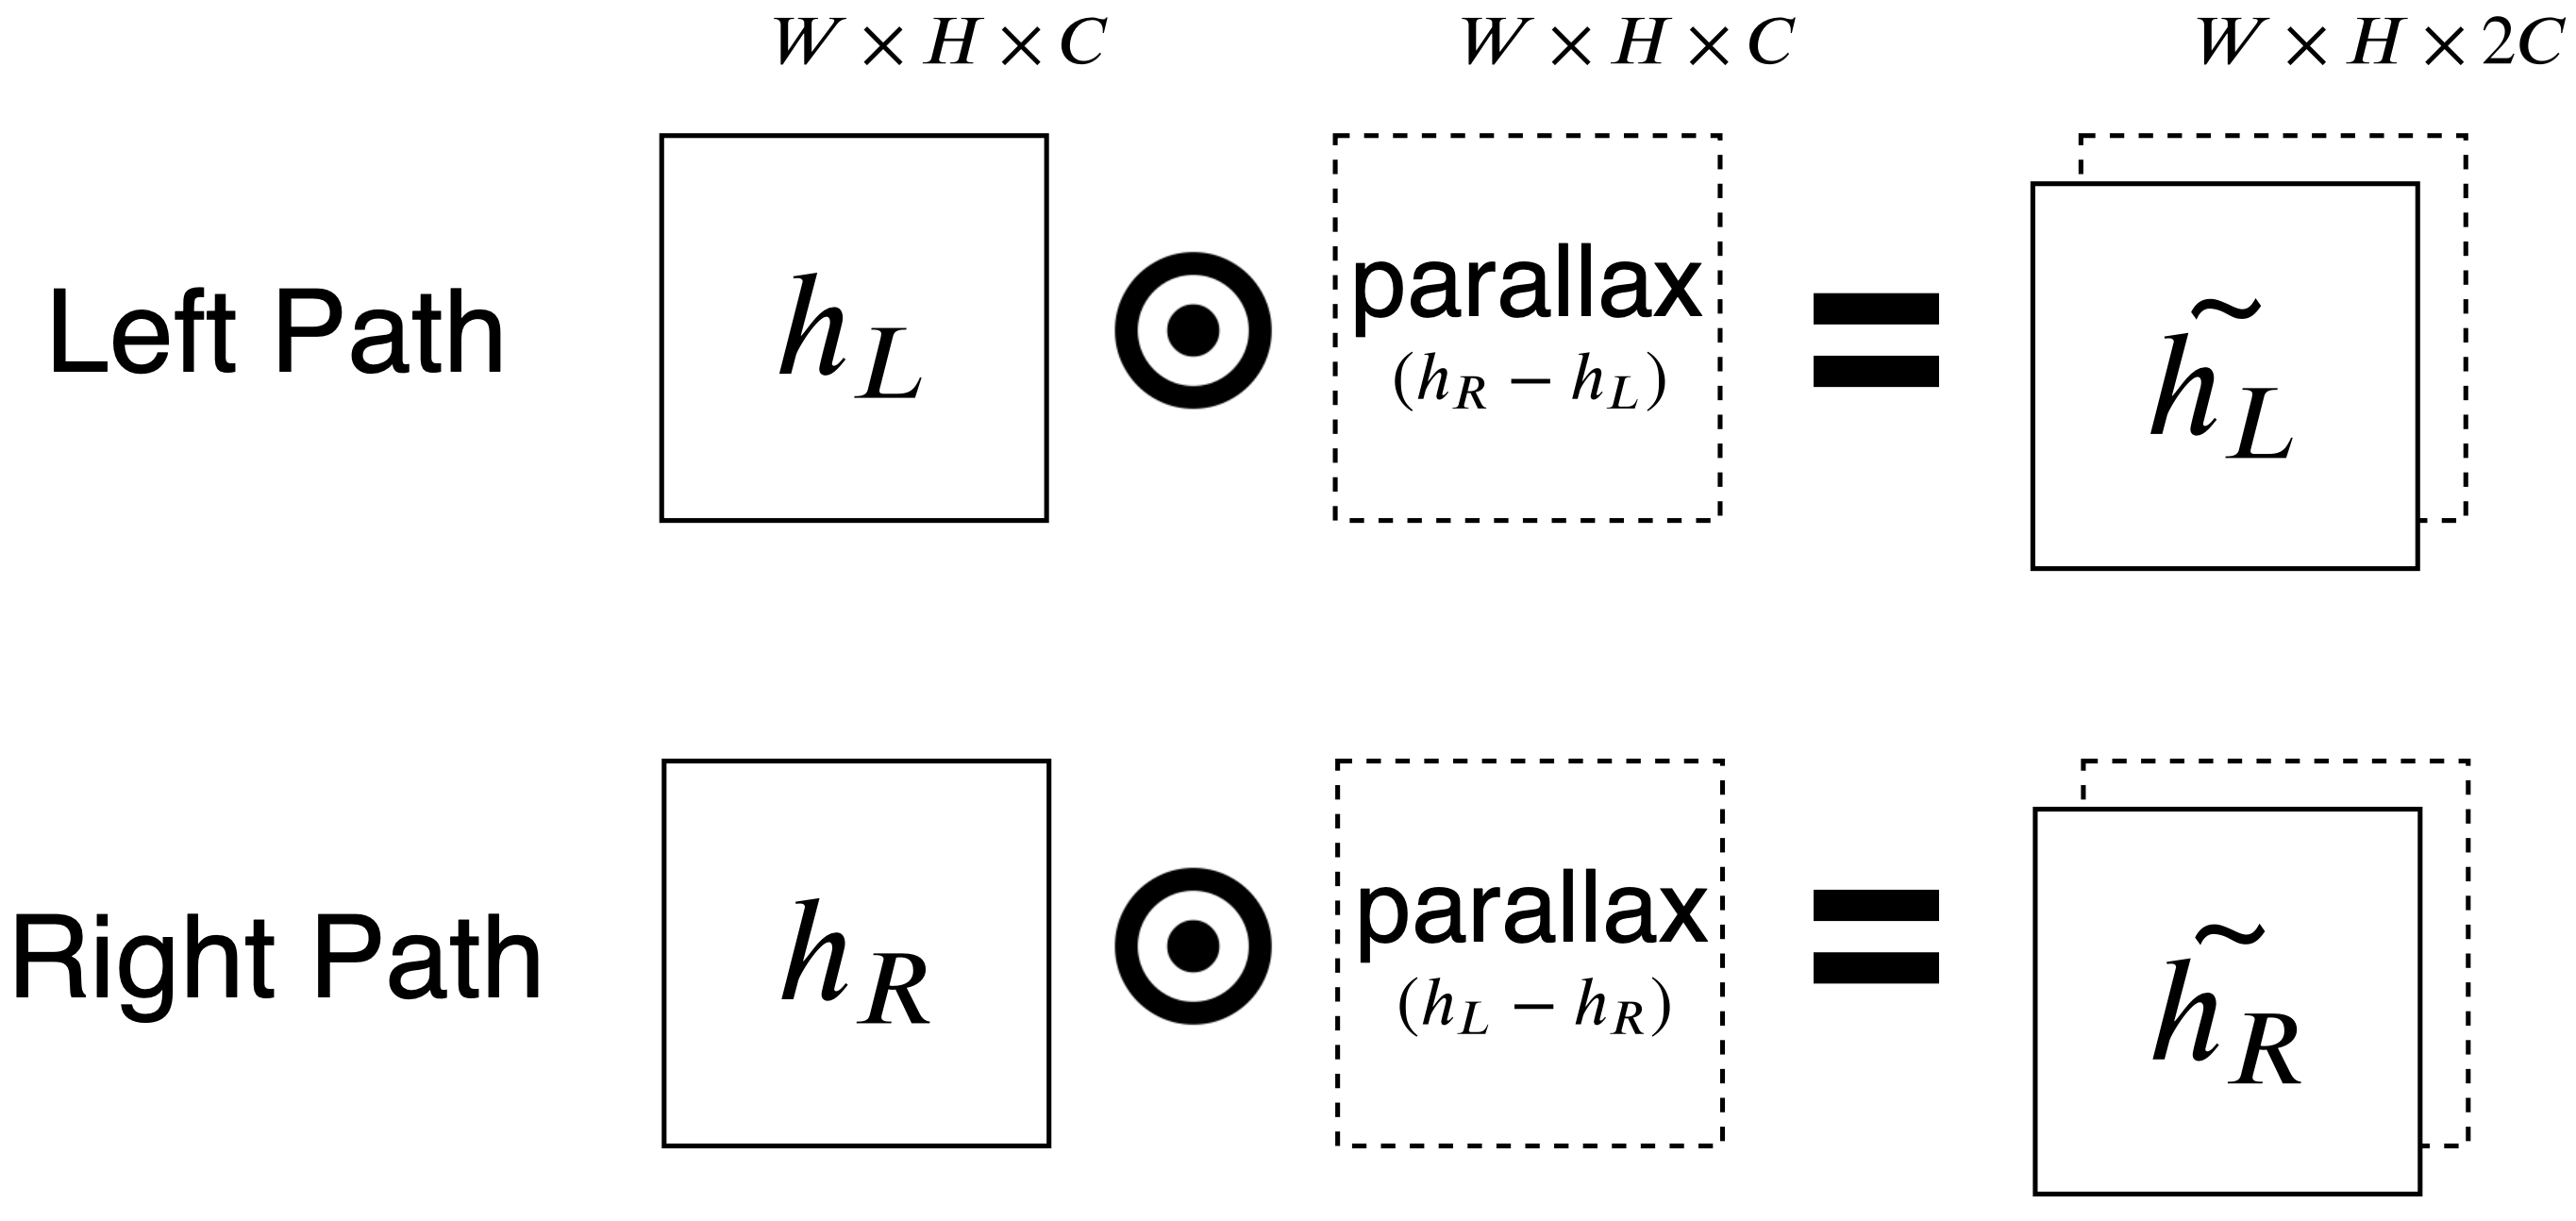
\includegraphics[width=0.6\textwidth]{parallax.png}
	\caption{Parallax augmentation}
	\label{fig:cnn2_parallax}
\end{figure}

Nello specifico, data una coppia di immagini binoculari, quella destra (\textit{h}\textsubscript{R}) viene combinata con \textit{h}\textsubscript{L} - \textit{h}\textsubscript{R}, mentre quella sinistra (\textit{h}\textsubscript{L}), con \textit{h}\textsubscript{R} - \textit{h}\textsubscript{L}: le due immagini \textit{aumentate} contengono le informazioni di entrambi gli occhi. \\
In figura~\ref{fig:dataset_augment_samples} vediamo degli esempio di \textit{parallax augmentation} di immagini prese dai vari dataset.
\begin{figure}[!ht]
	\centering
	\begin{subfigure}{0.4\textwidth}
		\begin{subcaptionblock}{1.2\textwidth}
			\centering
			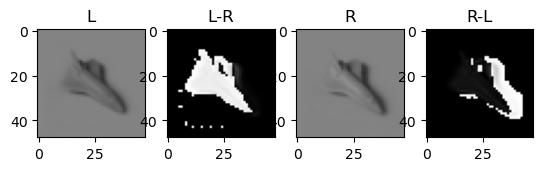
\includegraphics[width=1\linewidth]{smallnorb_augment_airplane.png}
			\caption{Aeroplano (small NORB)}
			\label{fig:smallnorb_augment_airplane}
		\end{subcaptionblock}%
		\hfill
		\begin{subcaptionblock}{1.2\textwidth}
			\centering
			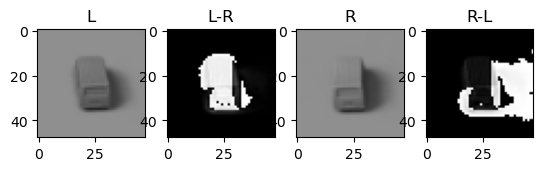
\includegraphics[width=1\linewidth]{smallnorb_augment_truck.png}
			\caption{Camion (small NORB)}
			\label{fig:smallnorb_augment_truck}
		\end{subcaptionblock}%
	\end{subfigure}
	\hfill
	\begin{subfigure}{0.4\textwidth}
		\begin{subcaptionblock}{1.2\textwidth}
			\centering
			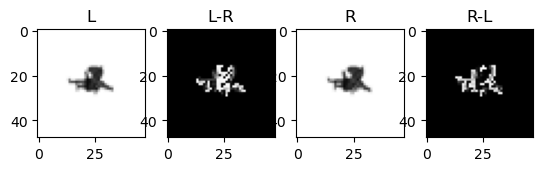
\includegraphics[width=1\linewidth]{modelnet_augment_airplane.png}
			\caption{Aeroplano (ModelNet)}
			\label{fig:modelnet_augment_airplane}
		\end{subcaptionblock}%
		\hfill
		\begin{subcaptionblock}{1.2\textwidth}
			\centering
			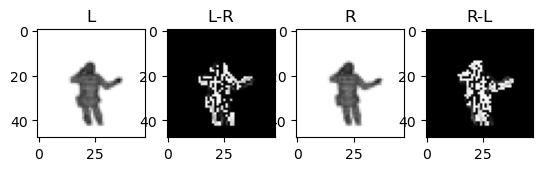
\includegraphics[width=1\linewidth]{modelnet_augment_human.png}
			\caption{Figura umana (ModelNet)}
			\label{fig:modelnet_augment_human}
		\end{subcaptionblock}%
	\end{subfigure}
	\hfill
	\begin{subfigure}{0.4\textwidth}
			\begin{subcaptionblock}{1.2\textwidth}
			\centering
			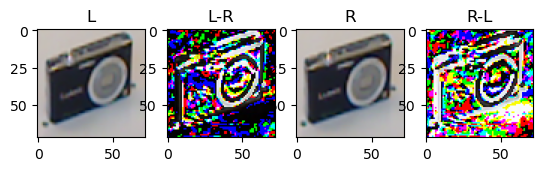
\includegraphics[width=1\linewidth]{rgbd_augment_camera.png}
			\caption{Macchina fotografica (RGB-D) }
			\label{fig:rgbd_augment_camera}
		\end{subcaptionblock}%
		\hfill
		\begin{subcaptionblock}{1.2\textwidth}
			\centering
			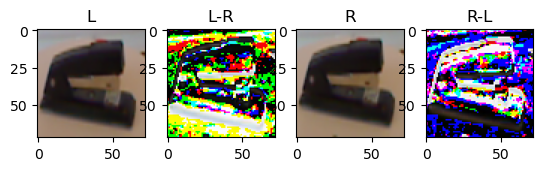
\includegraphics[width=1\linewidth]{rgbd_augment_stapler.png}
			\caption{Cucitrice (RGB-D)}
			\label{fig:rgbd_augment_stapler}
		\end{subcaptionblock}%
	\end{subfigure}
	\caption{Esempi di parallax augmentation}
	\label{fig:dataset_augment_samples}
\end{figure}

\noindent Ciascuna mappa aumentata viene immessa nel livello successivo attraverso il percorso sinistro o destro.
Questo consente ai filtri nei livelli convoluzionali di rilevare le caratteristiche stereoscopiche, osservando la parallasse e confrontando le parti nitide e sfocate.
Oltre alla \textit{parallax augmentation}, gli autori hanno introdotto un nuovo tipo di livello di \textit{pooling}, chiamato \textit{concentric multi-scale (CM) pooling}.
La figura~\ref{fig:cnn2_cmpooling} mostra come funziona il pooling CM: data un'immagine aumentata si ottengono delle mappe temporanee, alla quali si applica un operazione di \textit{max pooling}, per poi sovrapporsi lungo la dimensione del canale del tensore di input.
\begin{figure}[ht]
	\centering
	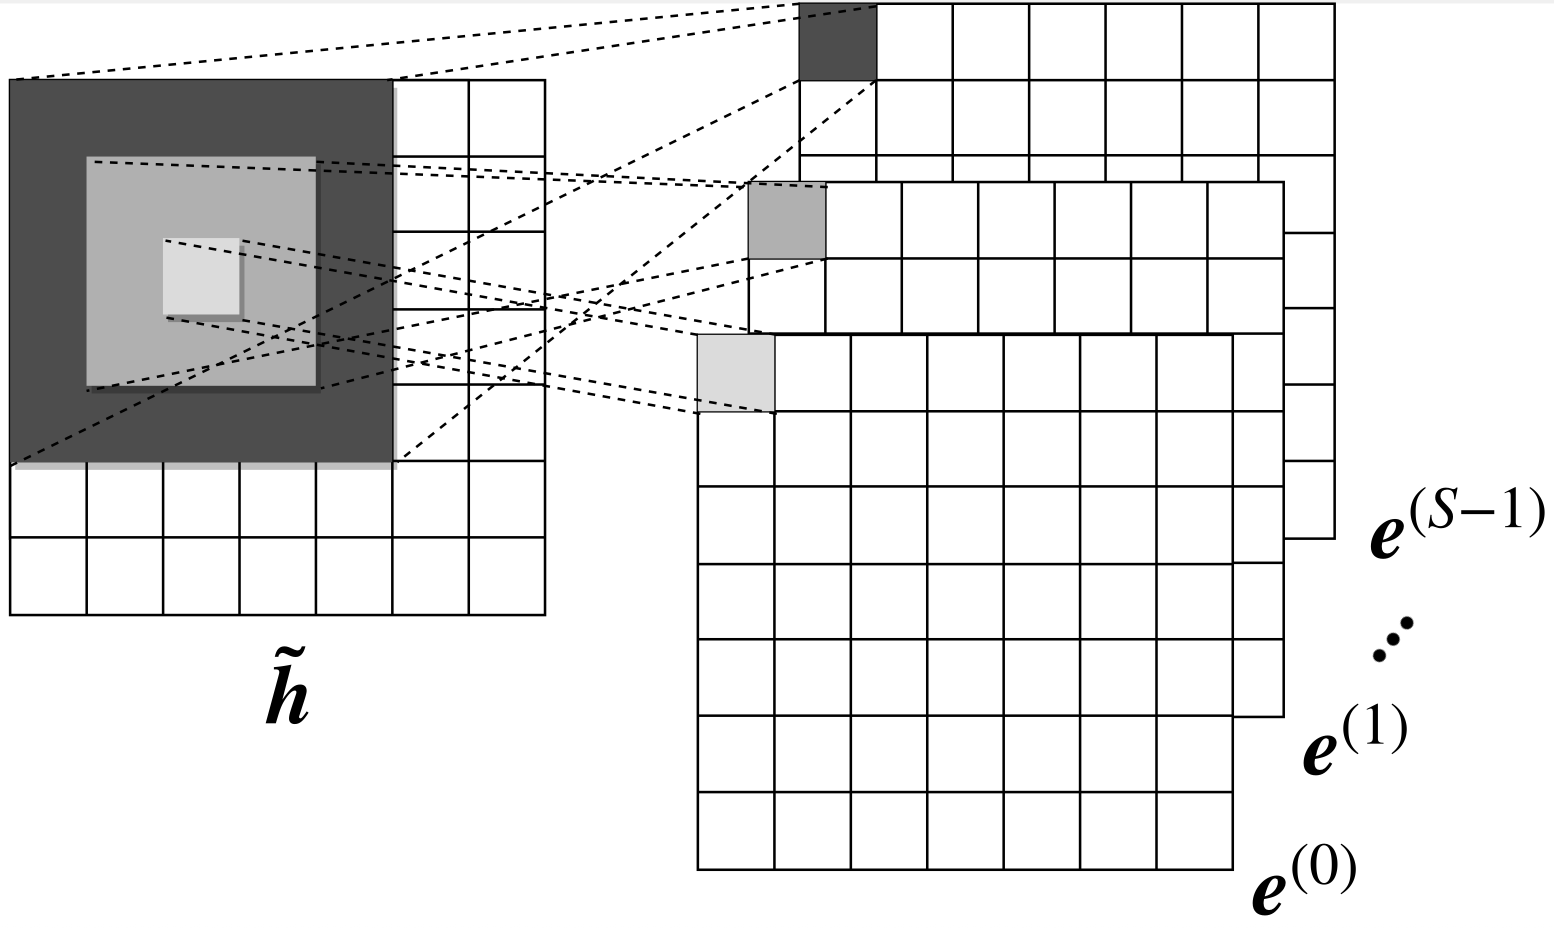
\includegraphics[width=0.6\textwidth]{cmpooling.png}
	\caption{CM Pooling}
	\label{fig:cnn2_cmpooling}
\end{figure}

\noindent A differenza dei livelli di pooling convenzionali che seguono i livelli convoluzionali, i livelli di pooling CM vengono posizionati prima di questi e non modificano la larghezza e l'altezza dell'immagine di input.
Questo aiuta il filtro nel livello successivo a rilevare facilmente i pattern stereoscopici, contrastando le caratteristiche sfocate dello sfondo con quelle nitide in primo piano.
In figura~\ref{fig:dataset_cmpooling_samples} vediamo un esempio di cosa succede alla fine del primo livello di CM a due immagini dei vari dataset.

\begin{figure}[ht]
	\begin{subfigure}{0.4\textwidth}
		\begin{subcaptionblock}{1.2\textwidth}
			\centering
			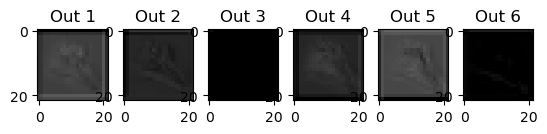
\includegraphics[width=1.2\linewidth]{smallnorb_M1_out_airplane.png}
			\caption{Aeroplano (small NORB)}
			\label{fig:smallnorb_M1_out_airplane}
		\end{subcaptionblock}%
		\hfill
		\begin{subcaptionblock}{1.2\textwidth}
			\centering
			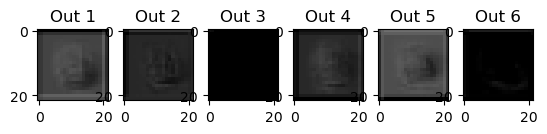
\includegraphics[width=1.2\linewidth]{smallnorb_M1_out_truck.png}
			\caption{Camion (small NORB)}
			\label{fig:smallnorb_M1_out_truck}
		\end{subcaptionblock}%
	\end{subfigure}
	\hfill
	\begin{subfigure}{0.4\textwidth}
		\begin{subcaptionblock}{1.2\textwidth}
			\centering
			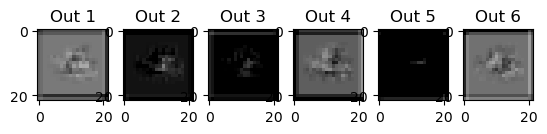
\includegraphics[width=1.2\linewidth]{modelnet_M1_out_airplane.png}
			\caption{Aeroplano (ModelNet)}
			\label{fig:modelnet_M1_out_airplane}
		\end{subcaptionblock}%
		\hfill
		\begin{subcaptionblock}{1.2\textwidth}
			\centering
			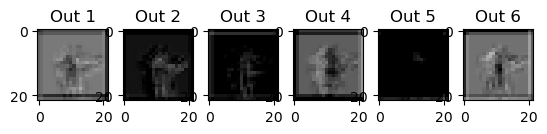
\includegraphics[width=1.2\linewidth]{modelnet_M1_out_human.png}
			\caption{Figura umana (ModelNet}
			\label{fig:modelnet_M1_out_human}
		\end{subcaptionblock}%
	\end{subfigure}
	\hfill
	\begin{subfigure}{0.4\textwidth}
		\begin{subcaptionblock}{1.2\textwidth}
			\centering
			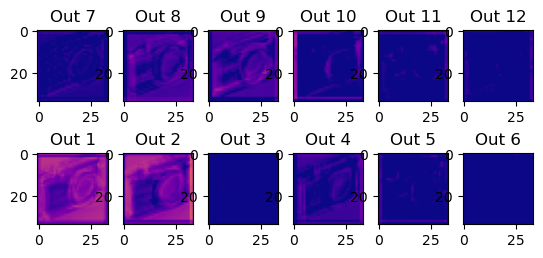
\includegraphics[width=1.2\linewidth]{rgbd_M1_out_camera.png}
			\caption{Macchina fotografica (RGB-D)}
			\label{fig:rgbd_M1_out_camera}
		\end{subcaptionblock}%
	\end{subfigure}
	\hfill
	\begin{subfigure}{0.4\textwidth}
		\begin{subcaptionblock}{1.2\textwidth}
			\centering
			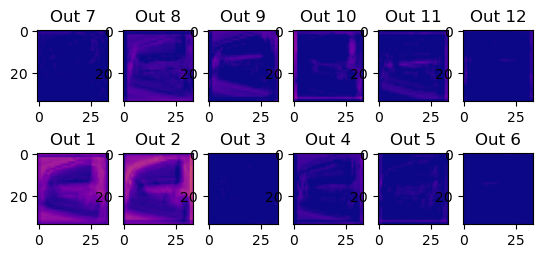
\includegraphics[width=1.2\linewidth]{rgbd_M1_out_stapler.png}
			\caption{Cucitrice (RGB-D)}
			\label{fig:rgbd_M1_out_stapler}
		\end{subcaptionblock}%
	\end{subfigure}
	\caption{Esempi di Concentric Multi-scale (CM) pooling}
	\label{fig:dataset_cmpooling_samples}
\end{figure}

\newpage
\subsubsection{Parametri}
All'interno dell'articolo\cite{neurips2019:cnn2} e del materiale supplementare\cite{cnn2:supplementary} gli autori hanno descritto parte della struttura del modello e i parametri utilizzati per realizzarla.

\begin{foreigndisplaycquote}{english}[\S3.2]{cnn2:supplementary}
We train each model using Adam algorithm ($\ldots$) with mini-batches of size 32.
We use early stopping strategy for all experiments.\\
$\ldots$\\
Our CNN\textsuperscript{2} consists of 3 blocks. Each block has a CM pooling layer and a convolution layer.
We use 3 scales (s = 0, 1, 2) in a CM pooling layer.
The first, second, and third convolution layers have 6, 12, and 32 filters with sizes 5 x 5, 5 × 5, and 3 x 3 respectively.
All filters use the stride of 1, and each unit uses the ReLU non-linearity.
\end{foreigndisplaycquote}
Purtroppo non hanno inserito nessun dettaglio relativo al classificatore presente in figura~\ref{fig:cnn2_model} e non ci sono informazioni ne sulla configurazione dell'\textit{early stopping} ne sulla presenza o meno di un layer di \textit{dropout}.

Fortunatamente gli autori hanno messo a disposizione un repository\cite{cnn2:repository} su GitHub con il codice Python del modello, realizzato usando la libreria TensorFlow: in questo modo sono state ricavate le informazioni relative al classificatore e al layer di \textit{dropout}.
Non è stato possibile invece ricavare la configurazione dell'\textit{early stopping}, visto che non era presente nemmeno nel codice originale.

\section{Dataset}
Nel paper originale gli autori hanno addrestrato e testato il loro modello su tre diversi dataset: vediamoli in dettaglio.

\subsection{small NORB}
Questo dataset\cite{dataset:smallnorb}, destinato a esperimenti per il riconoscimento di oggetti 3D dalla loro forma, è composto da 48.600 immagini binoculari in scala di grigi di 50 giocattoli appartenenti a 5 diverse categorie.

\noindent Le categorie sono:
\begin{itemize}
	\item animali a 4 zampe
	\item figure umane
	\item aeroplani
	\item camion
	\item automobili
\end{itemize}
Ogni immagine binoculare è una coppia di file di grandezza 96x96 pixel.
\begin{figure}[!ht]
	\centerline{% center image to the page, not to text
		\begin{subcaptionblock}{0.4\textwidth}
			\centering
			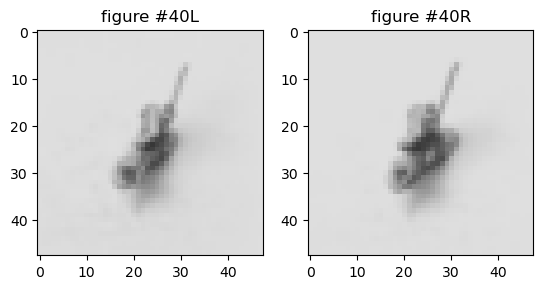
\includegraphics[width=1\linewidth]{smallnorb_figure.png}
			\caption{Figura umana}
			\label{fig:smallnorb_figure}
		\end{subcaptionblock}%
		\begin{subcaptionblock}{0.4\textwidth}
			\centering
			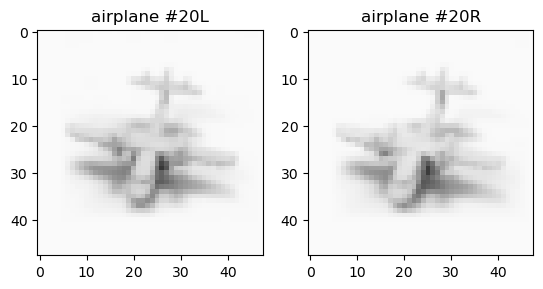
\includegraphics[width=1\linewidth]{smallnorb_airplane.png}
			\caption{Aeroplano}
			\label{fig:smallnorb_airplane}
		\end{subcaptionblock}%
		\begin{subcaptionblock}{0.4\textwidth}
			\centering
			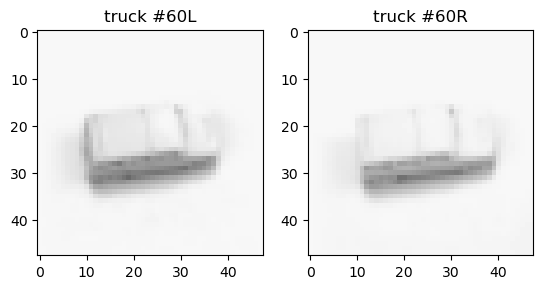
\includegraphics[width=1\linewidth]{smallnorb_truck.png}
			\caption{Camion}
			\label{fig:smallnorb_truck}
		\end{subcaptionblock}%
	}
	\caption{Esempi di immagini del dataset smallNORB}
	\label{fig:smallnorb_samples}
\end{figure}

\noindent Gli oggetti sono stati fotografati da una coppia di telecamere sotto 6 diverse condizioni di luce, 9 angolazioni (da 30 a 60 gradi, con passo 5 gradi) e 18 \textit{azimuth} (da 0 a 340 gradi con passo 20 gradi).
Il training set è composto da 5 istanze di ogni categoria (la 4, 6, 7, 8 e 9) e il test set dalle restanti (0, 1, 2, 3, e 5): ogni istanza ha 972 immagini binoculari.
In figura~\ref{fig:smallnorb_samples} possiamo vedere alcuni esempi di immagini del dataset.

\subsection{ModelNet2D}
Il dataset ModelNet40\cite{dataset:modelnet40} contiene circa 12.311 modelli CAD suddivisi in 40 classi.
Gli autori hanno selezionato 5 classi:
\begin{itemize}
	\item sedie
	\item figure umane
	\item aeroplani
	\item automobili
	\item lampade
\end{itemize}
e, per ciascuna classe, hanno preso 15 oggetti a caso.
Per ogni oggetto è stato fatto il render con 72 angoli di azimuth (con passo di 5 gradi), 9 angolazioni (da 30 a 70 gradi, con passo 5 gradi) sotto condizioni di luce fisse, per un totale di 648 immagini in scala di grigio.
\begin{figure}[!ht]
	\centerline{% center image to the page, not to text
		\begin{subcaptionblock}{0.4\textwidth}
			\centering
			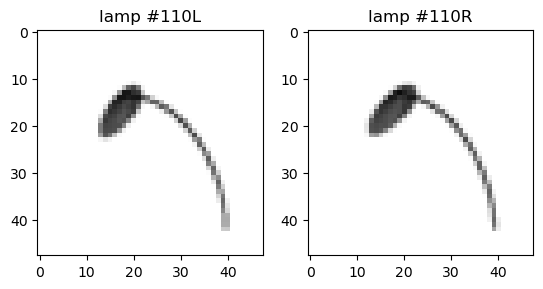
\includegraphics[width=1\linewidth]{modelnet_lamp.png}
			\caption{Lampada}
			\label{fig:modelnet2d_lamp}
		\end{subcaptionblock}%
		\begin{subcaptionblock}{0.4\textwidth}
			\centering
			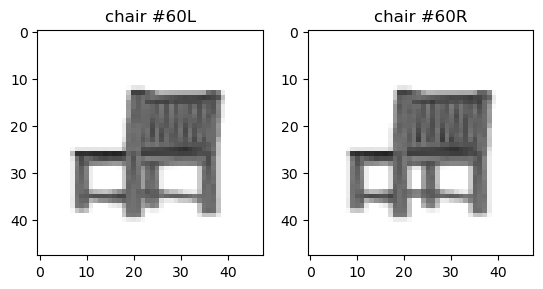
\includegraphics[width=1\linewidth]{modelnet_chair.png}
			\caption{Sedia}
			\label{fig:modelnet2d_chair}
		\end{subcaptionblock}%
		\begin{subcaptionblock}{0.4\textwidth}
			\centering
			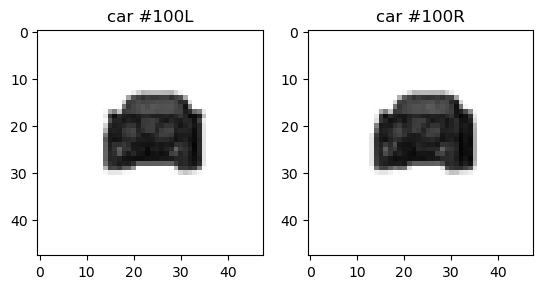
\includegraphics[width=1\linewidth]{modelnet_car.png}
			\caption{Automobile}
			\label{fig:modelnet2d_car}
		\end{subcaptionblock}%
	}
	\caption{Esempi di immagini del dataset ModelNet2d}
	\label{fig:modelnet2d_samples}
\end{figure}
Nell'articolo, gli autori affermano che le immagini hanno una risoluzione di 96 x 96 pixel ma, nel dataset fornito, hanno una risoluzione di 144 x 144 pixel.
Seguendo questi passaggi, hanno ottenuto 48.600 immagini: questo subset è stato chiamato dagli autori ModelNet2D.
In figura~\ref{fig:modelnet2d_samples} possiamo vedere alcuni esempi di immagini del dataset.

\subsection{RGB-D Object}
Questo dataset\cite{dataset:rgb-d} è composto da 300 oggetti di uso comune divisi in 51 classi.
Gli autori hanno selezionato 5 classi:
\begin{itemize}
	\item macchine fotografiche
	\item torce elettriche
	\item lampadine
	\item brocche
	\item cucitrici
\end{itemize}
È stato creato usando una macchina fotografica di tipo 3D Kinect a colori RGB con una risoluzione di 640x480 pixel.
Ogni oggetto è stato posizionato su una piattaforma girevole ed è stata acquisita la sequenza video di una rotazione completa.
Per ogni oggetto, sono presenti 3 sequenze video, ciascuna registrata con la telecamera montata a un'altezza diversa in modo che l'oggetto sia visto da angolazioni diverse.
Nel dataset sono presenti immagini degli oggetti, prese con angoli multipli di 10 gradi, ottenendo un totale di 250.000 immagini a colori.
In figura~\ref{fig:rgbd_samples} possiamo vedere alcuni esempi di immagini del dataset.
\begin{figure}[!ht]
	\centerline{% center image to the page, not to text
		\begin{subcaptionblock}{0.4\textwidth}
			\centering
			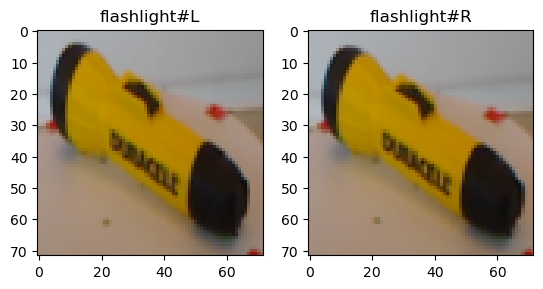
\includegraphics[width=1\linewidth]{rgbd_flashlight.png}
			\caption{Torcia elettrica}
			\label{fig:rgbd_flashlight}
		\end{subcaptionblock}%
		\begin{subcaptionblock}{0.4\textwidth}
			\centering
			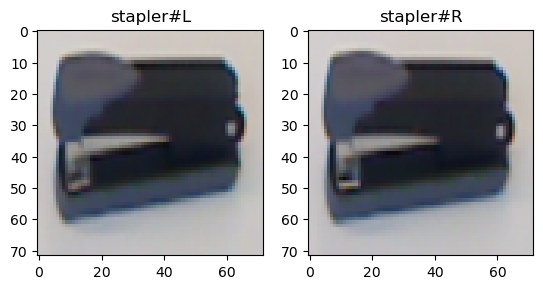
\includegraphics[width=1\linewidth]{rgbd_stapler.png}
			\caption{Cucitrice}
			\label{fig:rgbd_stapler}
		\end{subcaptionblock}%
		\begin{subcaptionblock}{0.4\textwidth}
			\centering
			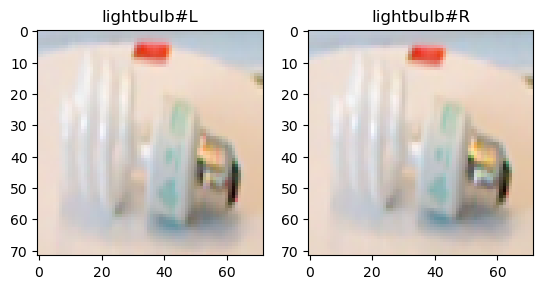
\includegraphics[width=1\linewidth]{rgbd_lightbulb}
			\caption{Lampadina}
			\label{fig:rgbd_lightbulb}
		\end{subcaptionblock}%
	}
	\caption{Esempi di immagini del dataset RGB-D}
	\label{fig:rgbd_samples}
\end{figure}
Nell'articolo, gli autori affermano che le immagini hanno una risoluzione di 640 x 480 pixel ma, nel dataset fornito (solo in parte) e nel codice, hanno utilizzato la versione \textit{cropped}, cioè quella dove si vede solo l'oggetto: queste immagini hanno una risoluzione massima di 144 x 144 pixel.
\section{Risultati ottenuti}

\subsection{small NORB}

\subsubsection{Codice originale}
Il codice originale presente nel repository degli autori differisce da quanto scritto nell'articolo: in particolare, la divisione del dataset non è la stessa.
Nell'articolo viene definita in questo modo:

\begin{foreigndisplaycquote}{english}[\S4.1]{neurips2019:cnn2}
On the SmallNORB dataset, we use the images taken from azimuths of degrees from 20 to 80 as the training set, degrees at 0 and 100 as the validation set, and the rest as the test set.
\end{foreigndisplaycquote}
mentre nel codice, il training set è pari a \(\frac{1}{3}\) di tutte le immagini (16200) e il test set è composto da tutto il resto (32400).
Nel codice manca completamente il validation set.
\begin{table}[!ht]
	\centering
	\begin{tabular}[t]{|c|cc|}
		\hline
		& \textbf{Accuracy} & \textbf{Loss} \\
		\hline
		training set codice autori& 0.888 & 1.727 \\
		training set articolo& 0.775 & 6.631 \\
		training set maggiore& 0.958 & 0.397 \\
		articolo & \textbf{0.865} & - \\
		\hline
	\end{tabular}
	\caption{Test loss/accuracy smallNORB (con validation set)}
	\label{tab:smallnorb_val_loss_acc}
\end{table}

\noindent Utilizzando la suddivisione del dataset presente nel codice (training set: 16200, test set: 32400), il risultato è quello nella prima riga della tabella~\ref{tab:smallnorb_val_loss_acc}, abbastanza in linea con quanto scritto nell'articolo.
\begin{figure}[!ht]
	\centerline{% center image to the page, not to text
		\begin{subcaptionblock}{0.6\textwidth}
			\centering
			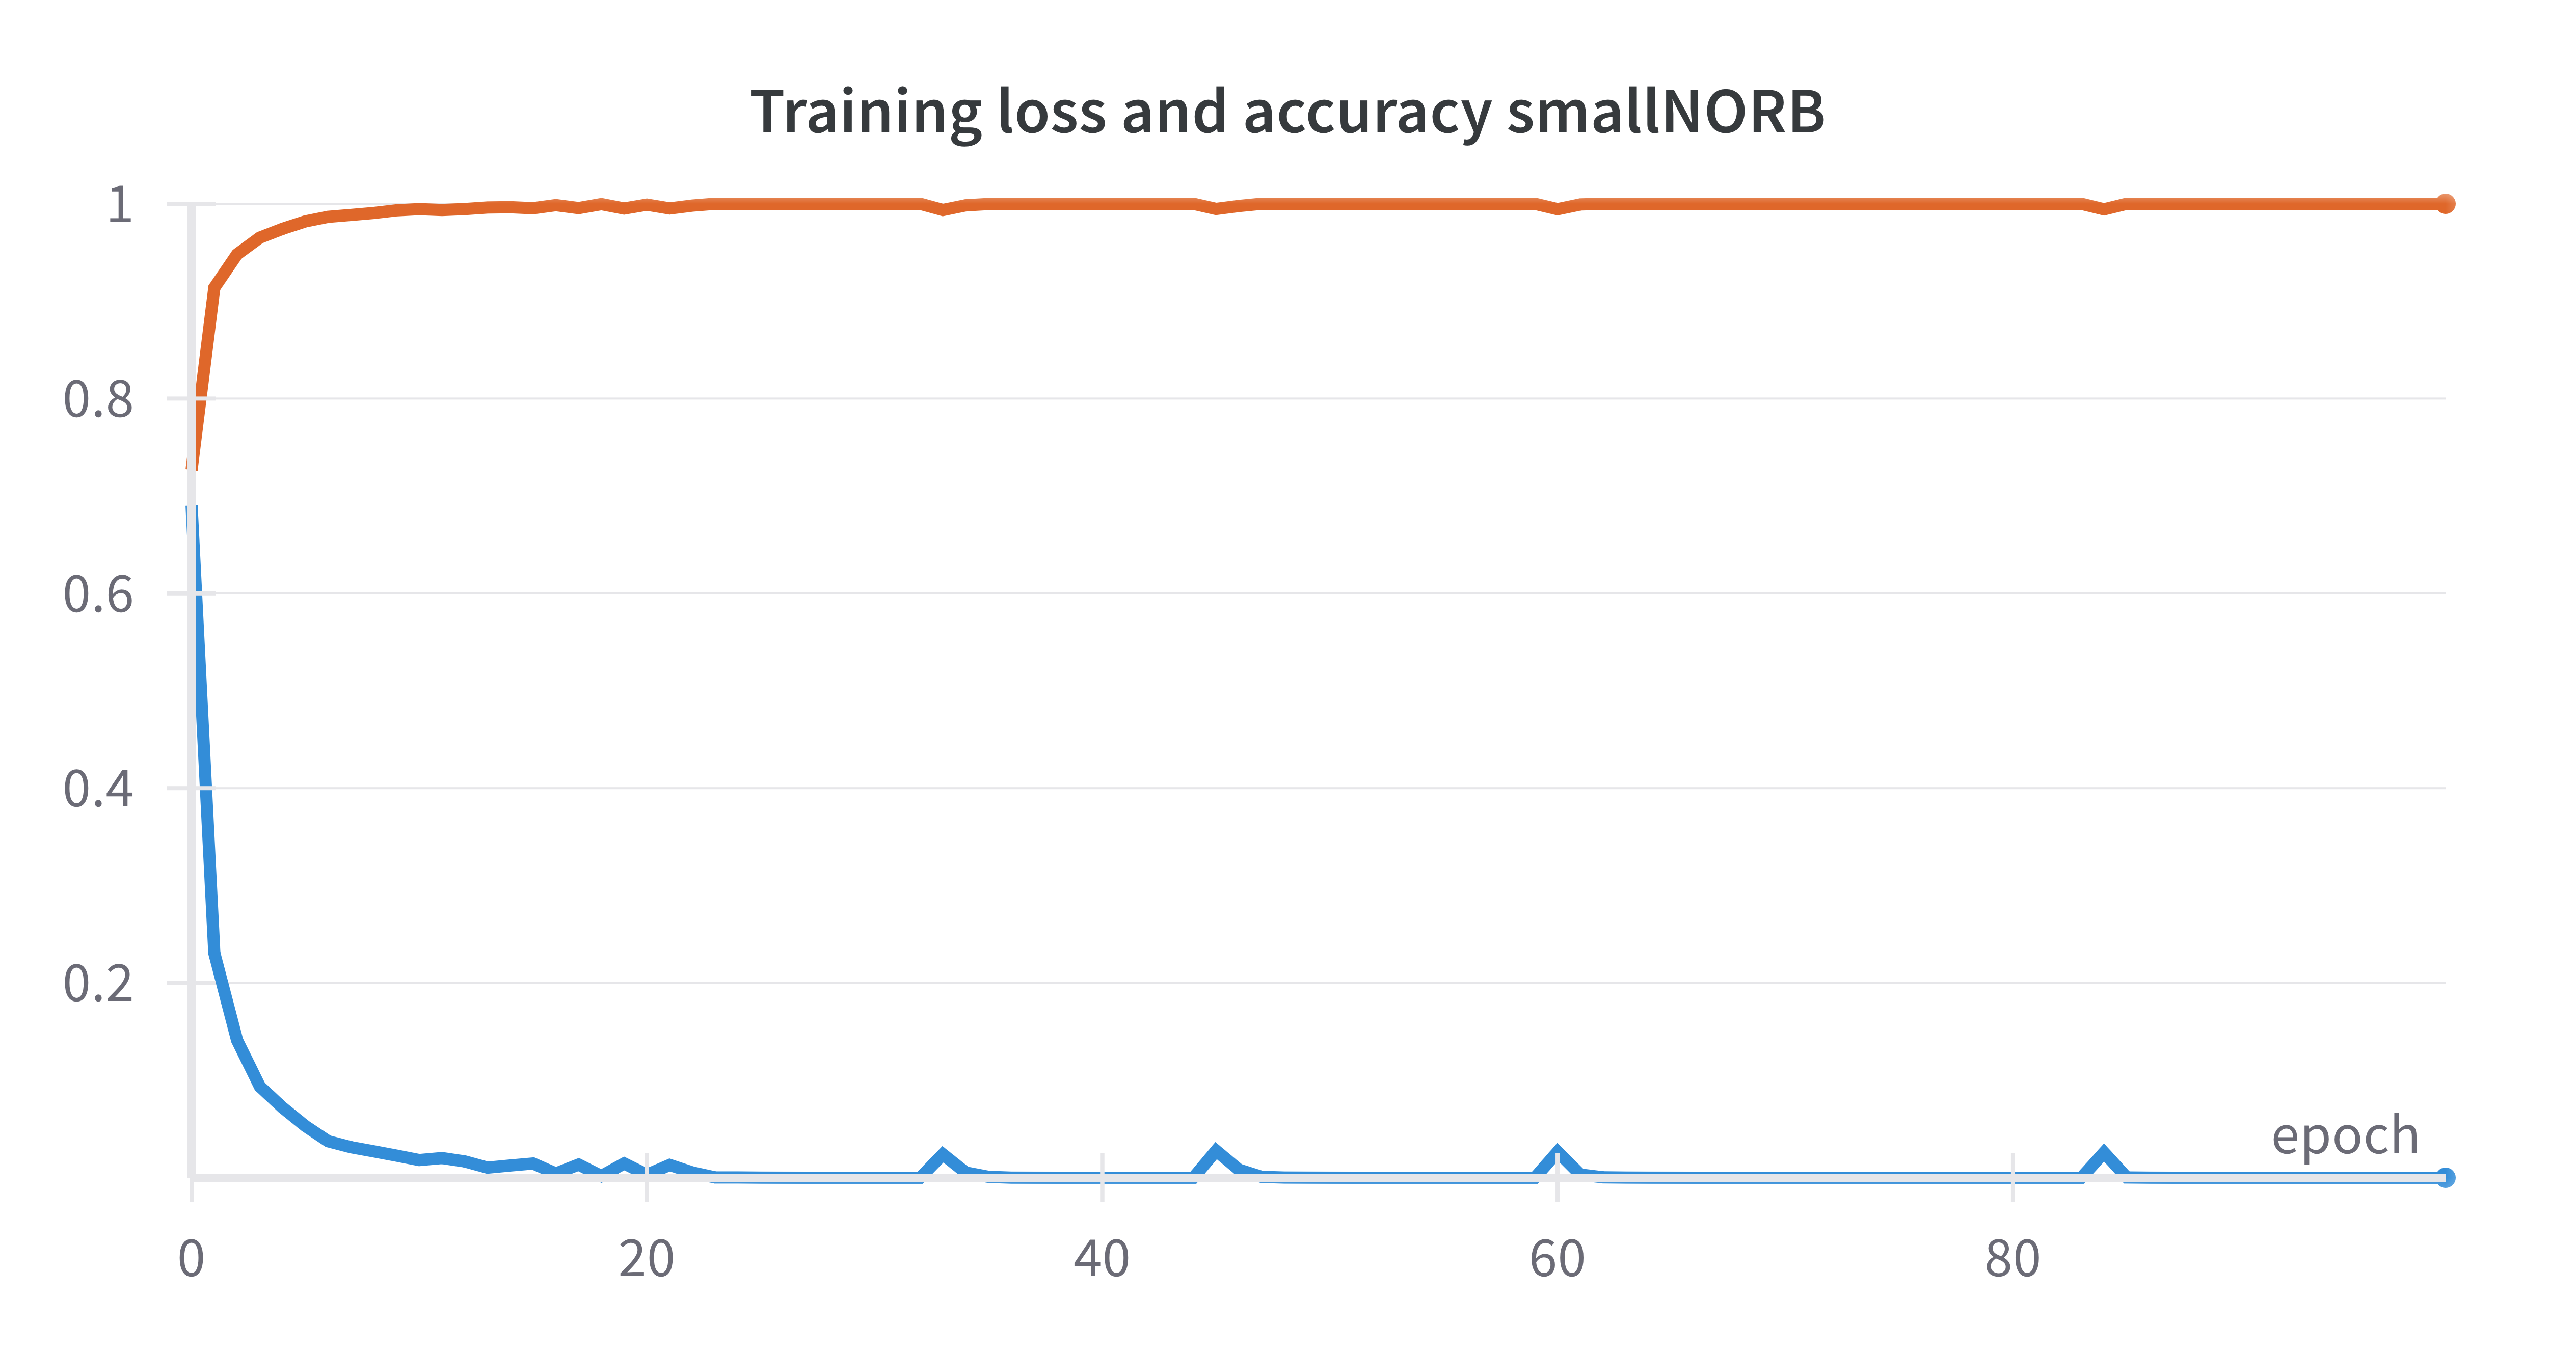
\includegraphics[width=0.9\linewidth]{smallnorb_train_loss_acc_original.png}
			\caption{Training  loss/accuracy}
			\label{fig:smallnorb_train_loss_acc_original}
		\end{subcaptionblock}%
		\begin{subcaptionblock}{0.6\textwidth}
			\centering
			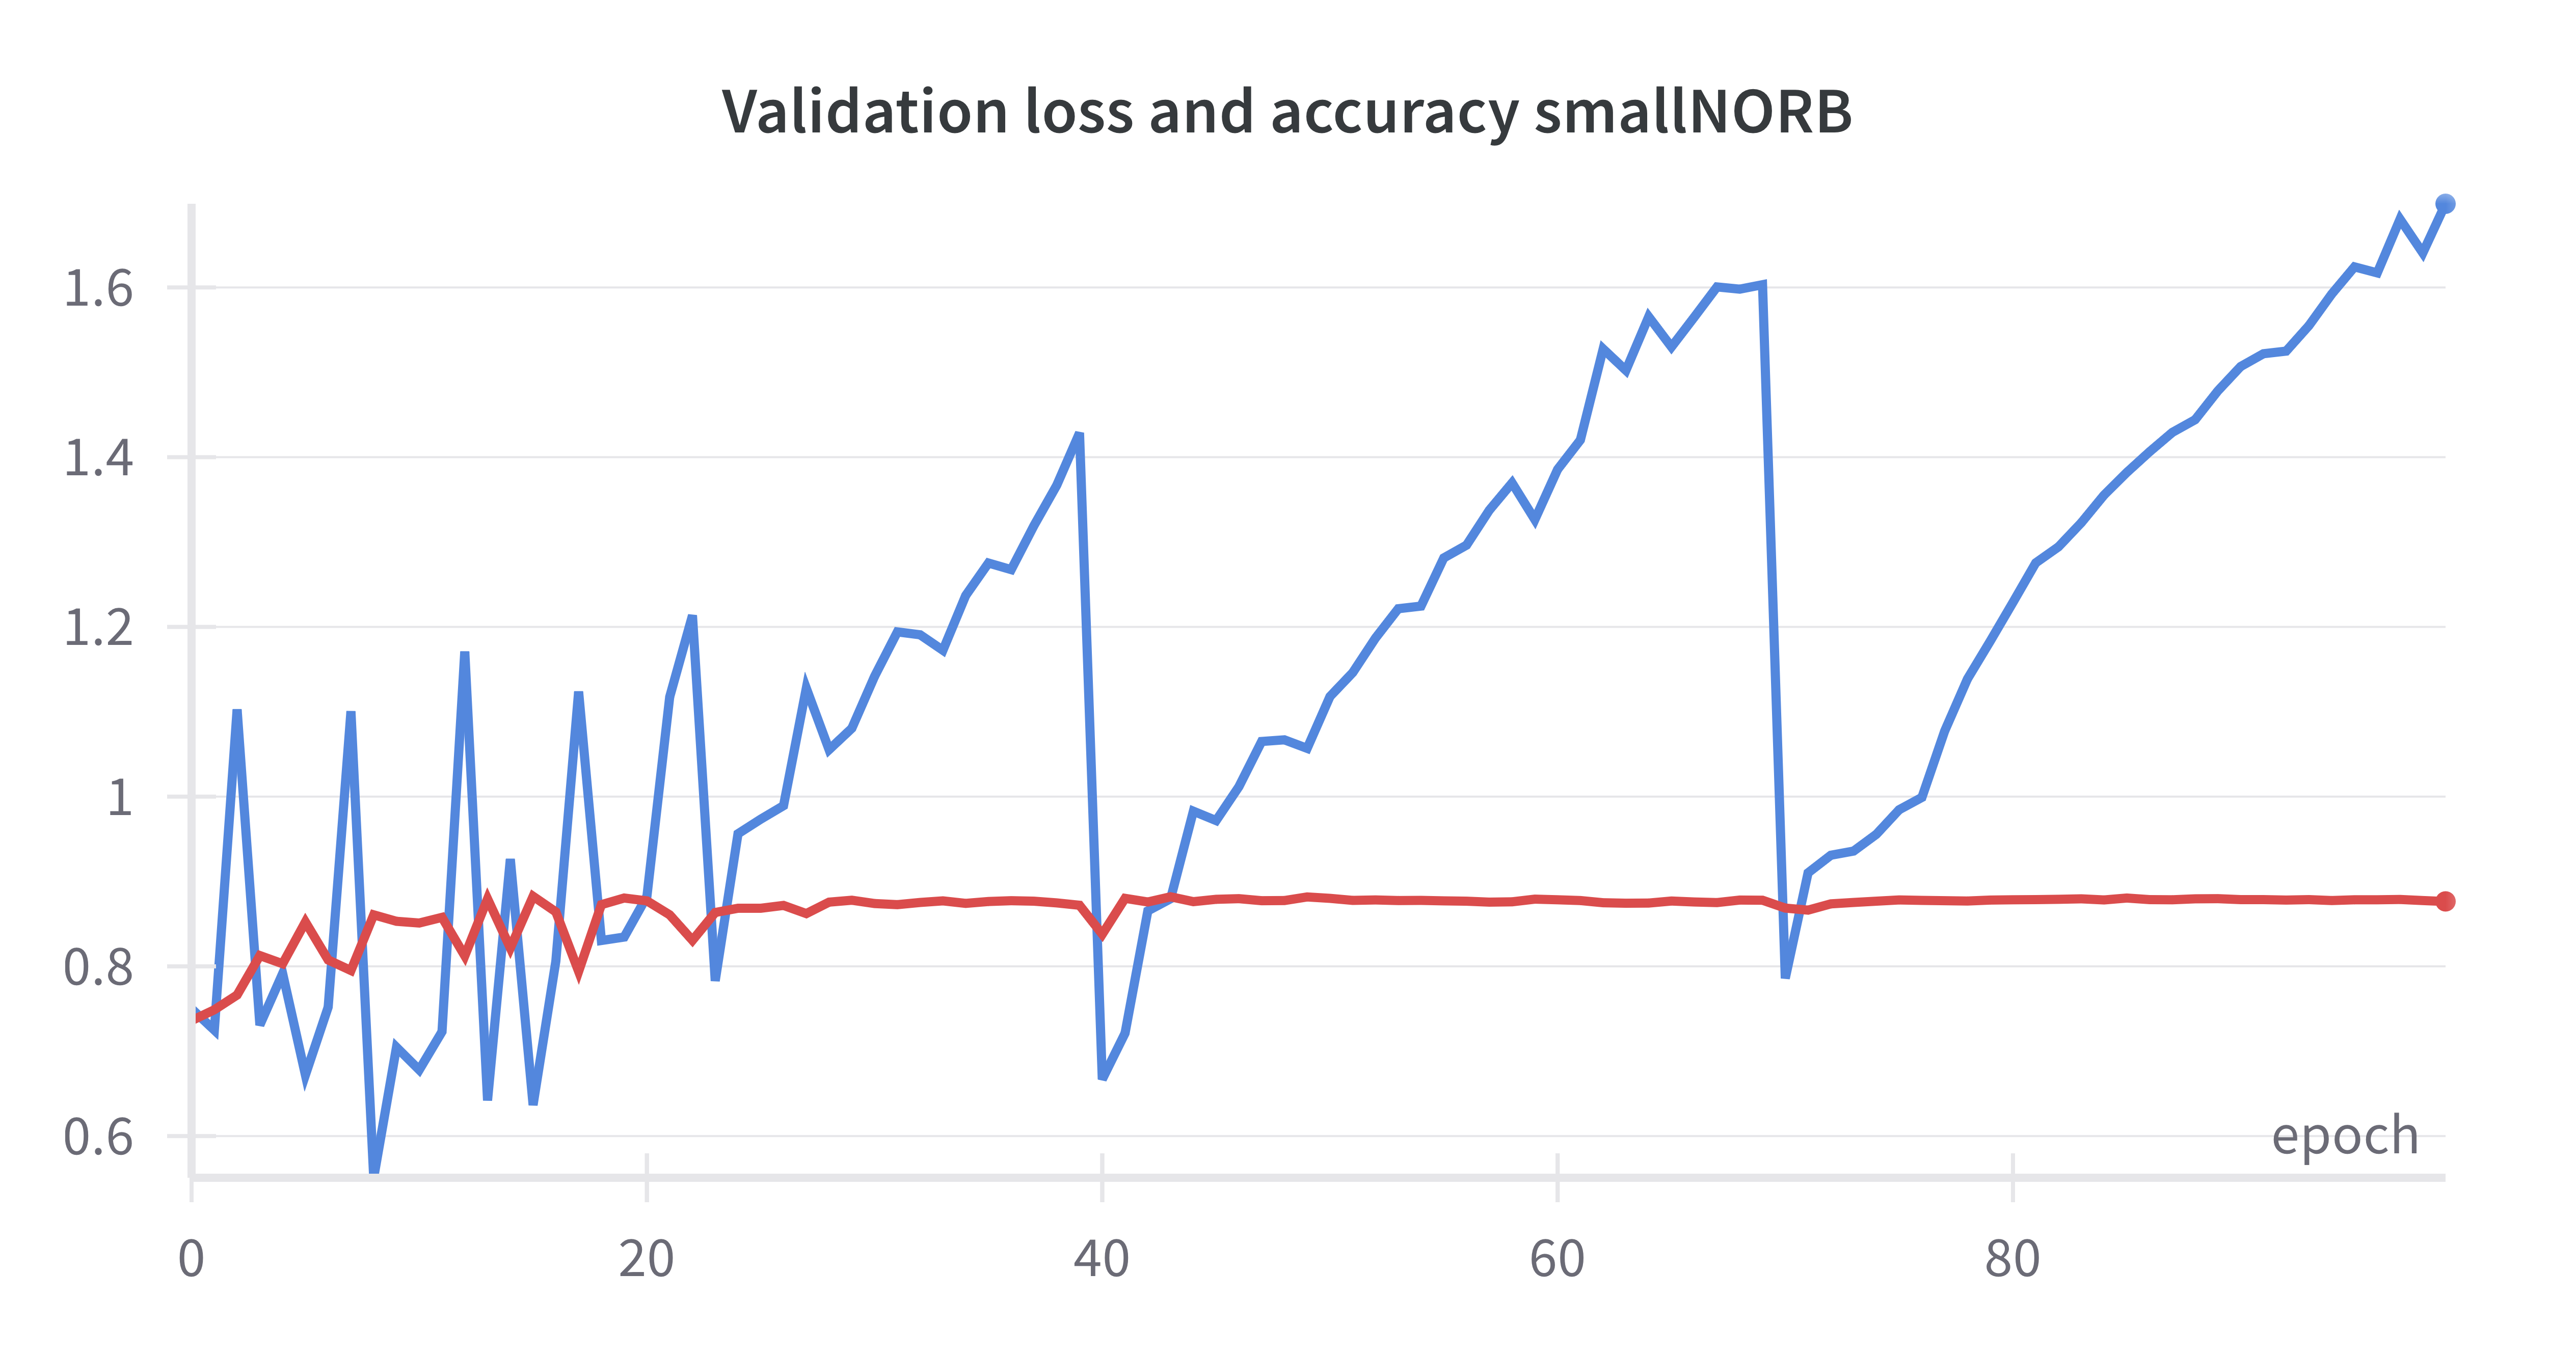
\includegraphics[width=0.9\linewidth]{smallnorb_val_loss_acc_original.png}
			\caption{Validation loss/accuracy}
			\label{fig:smallnorb_val_loss_acc_original}
		\end{subcaptionblock}%
	}
	\caption{Metriche del dataset smallNORB (con validation set)}
	\label{fig:smallnorb_train_val_loss_acc_original}
\end{figure}
Invece, modificando il codice originale (per suddividere il dataset come descritto nell'articolo, cioè training set: 10800, validation set: 5400 e test set: 32400), il risultato cambia, come si può vedere nella seconda riga della tabella~\ref{tab:smallnorb_val_loss_acc}.
Usando la suddivisione del dataset indicata nell'articolo possiamo osservare che la validation loss ha una curva anomala (figura~\ref{fig:smallnorb_train_val_loss_acc_original}).
\begin{figure}[!ht]
	\centerline{% center image to the page, not to text
		\begin{subcaptionblock}{.6\textwidth}
			\centering
			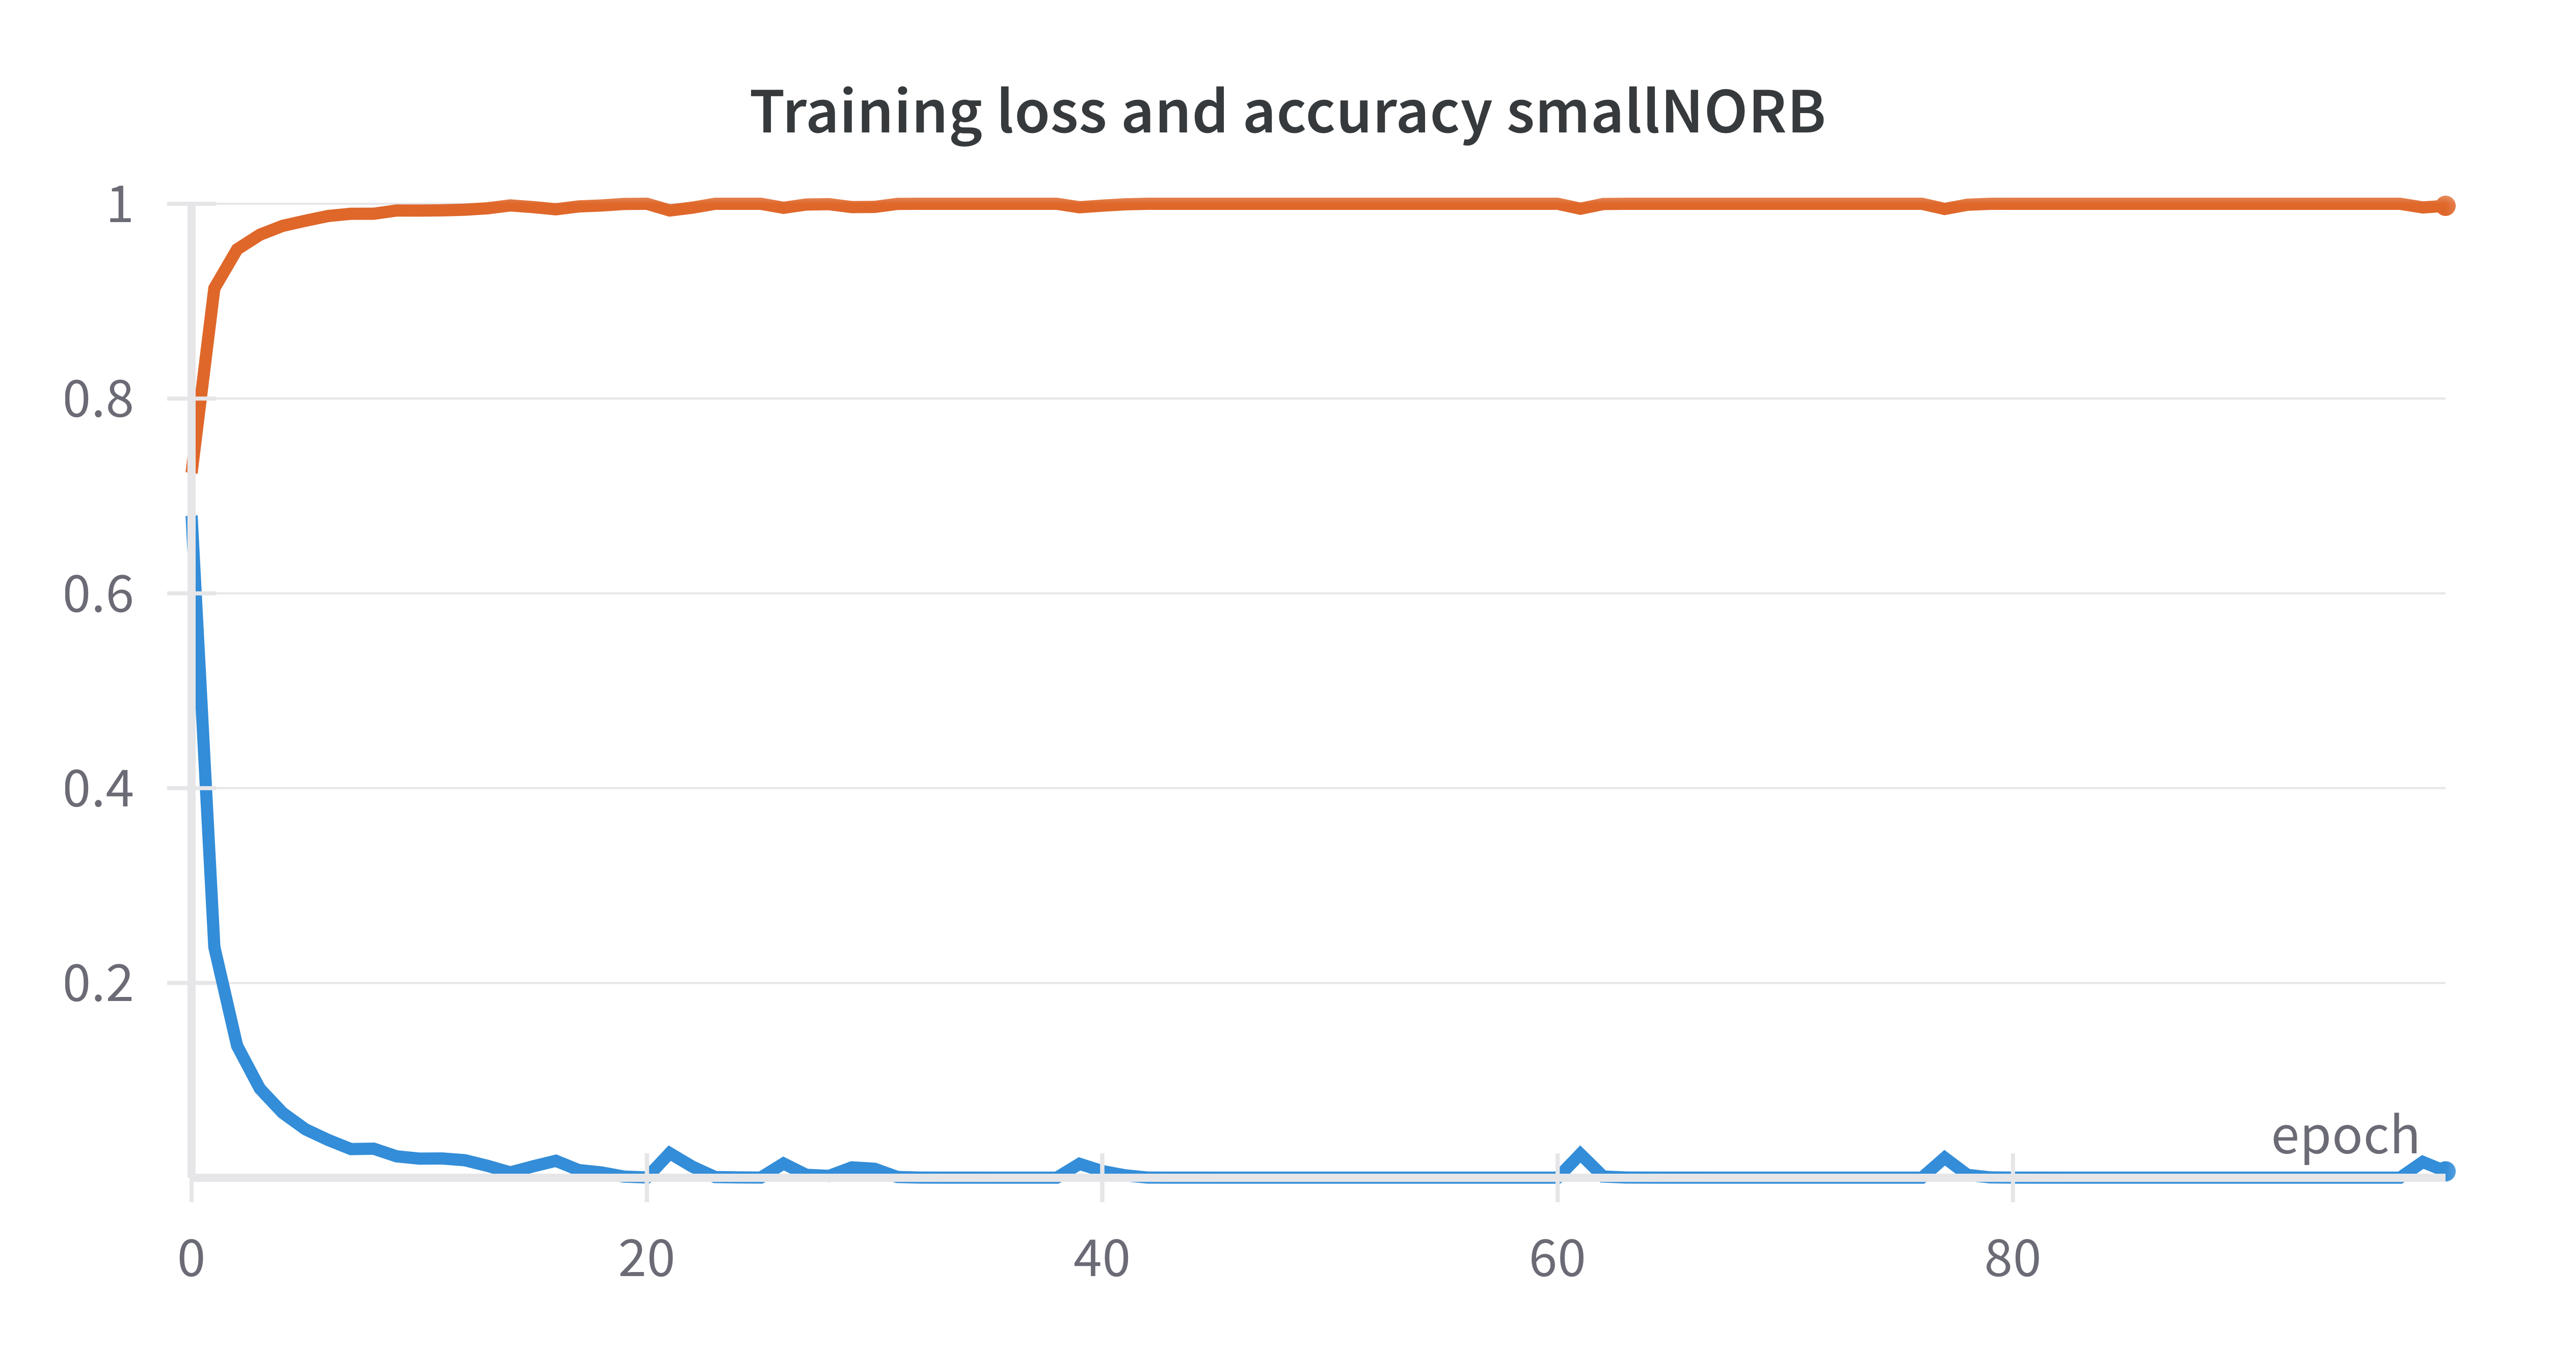
\includegraphics[width=1\linewidth]{smallnorb_train_loss_acc_mod.png}
			\caption{Training  loss/accuracy}
			\label{fig:smallnorb_train_loss_acc_mod}
		\end{subcaptionblock}%
		\begin{subcaptionblock}{.6\textwidth}
			\centering
			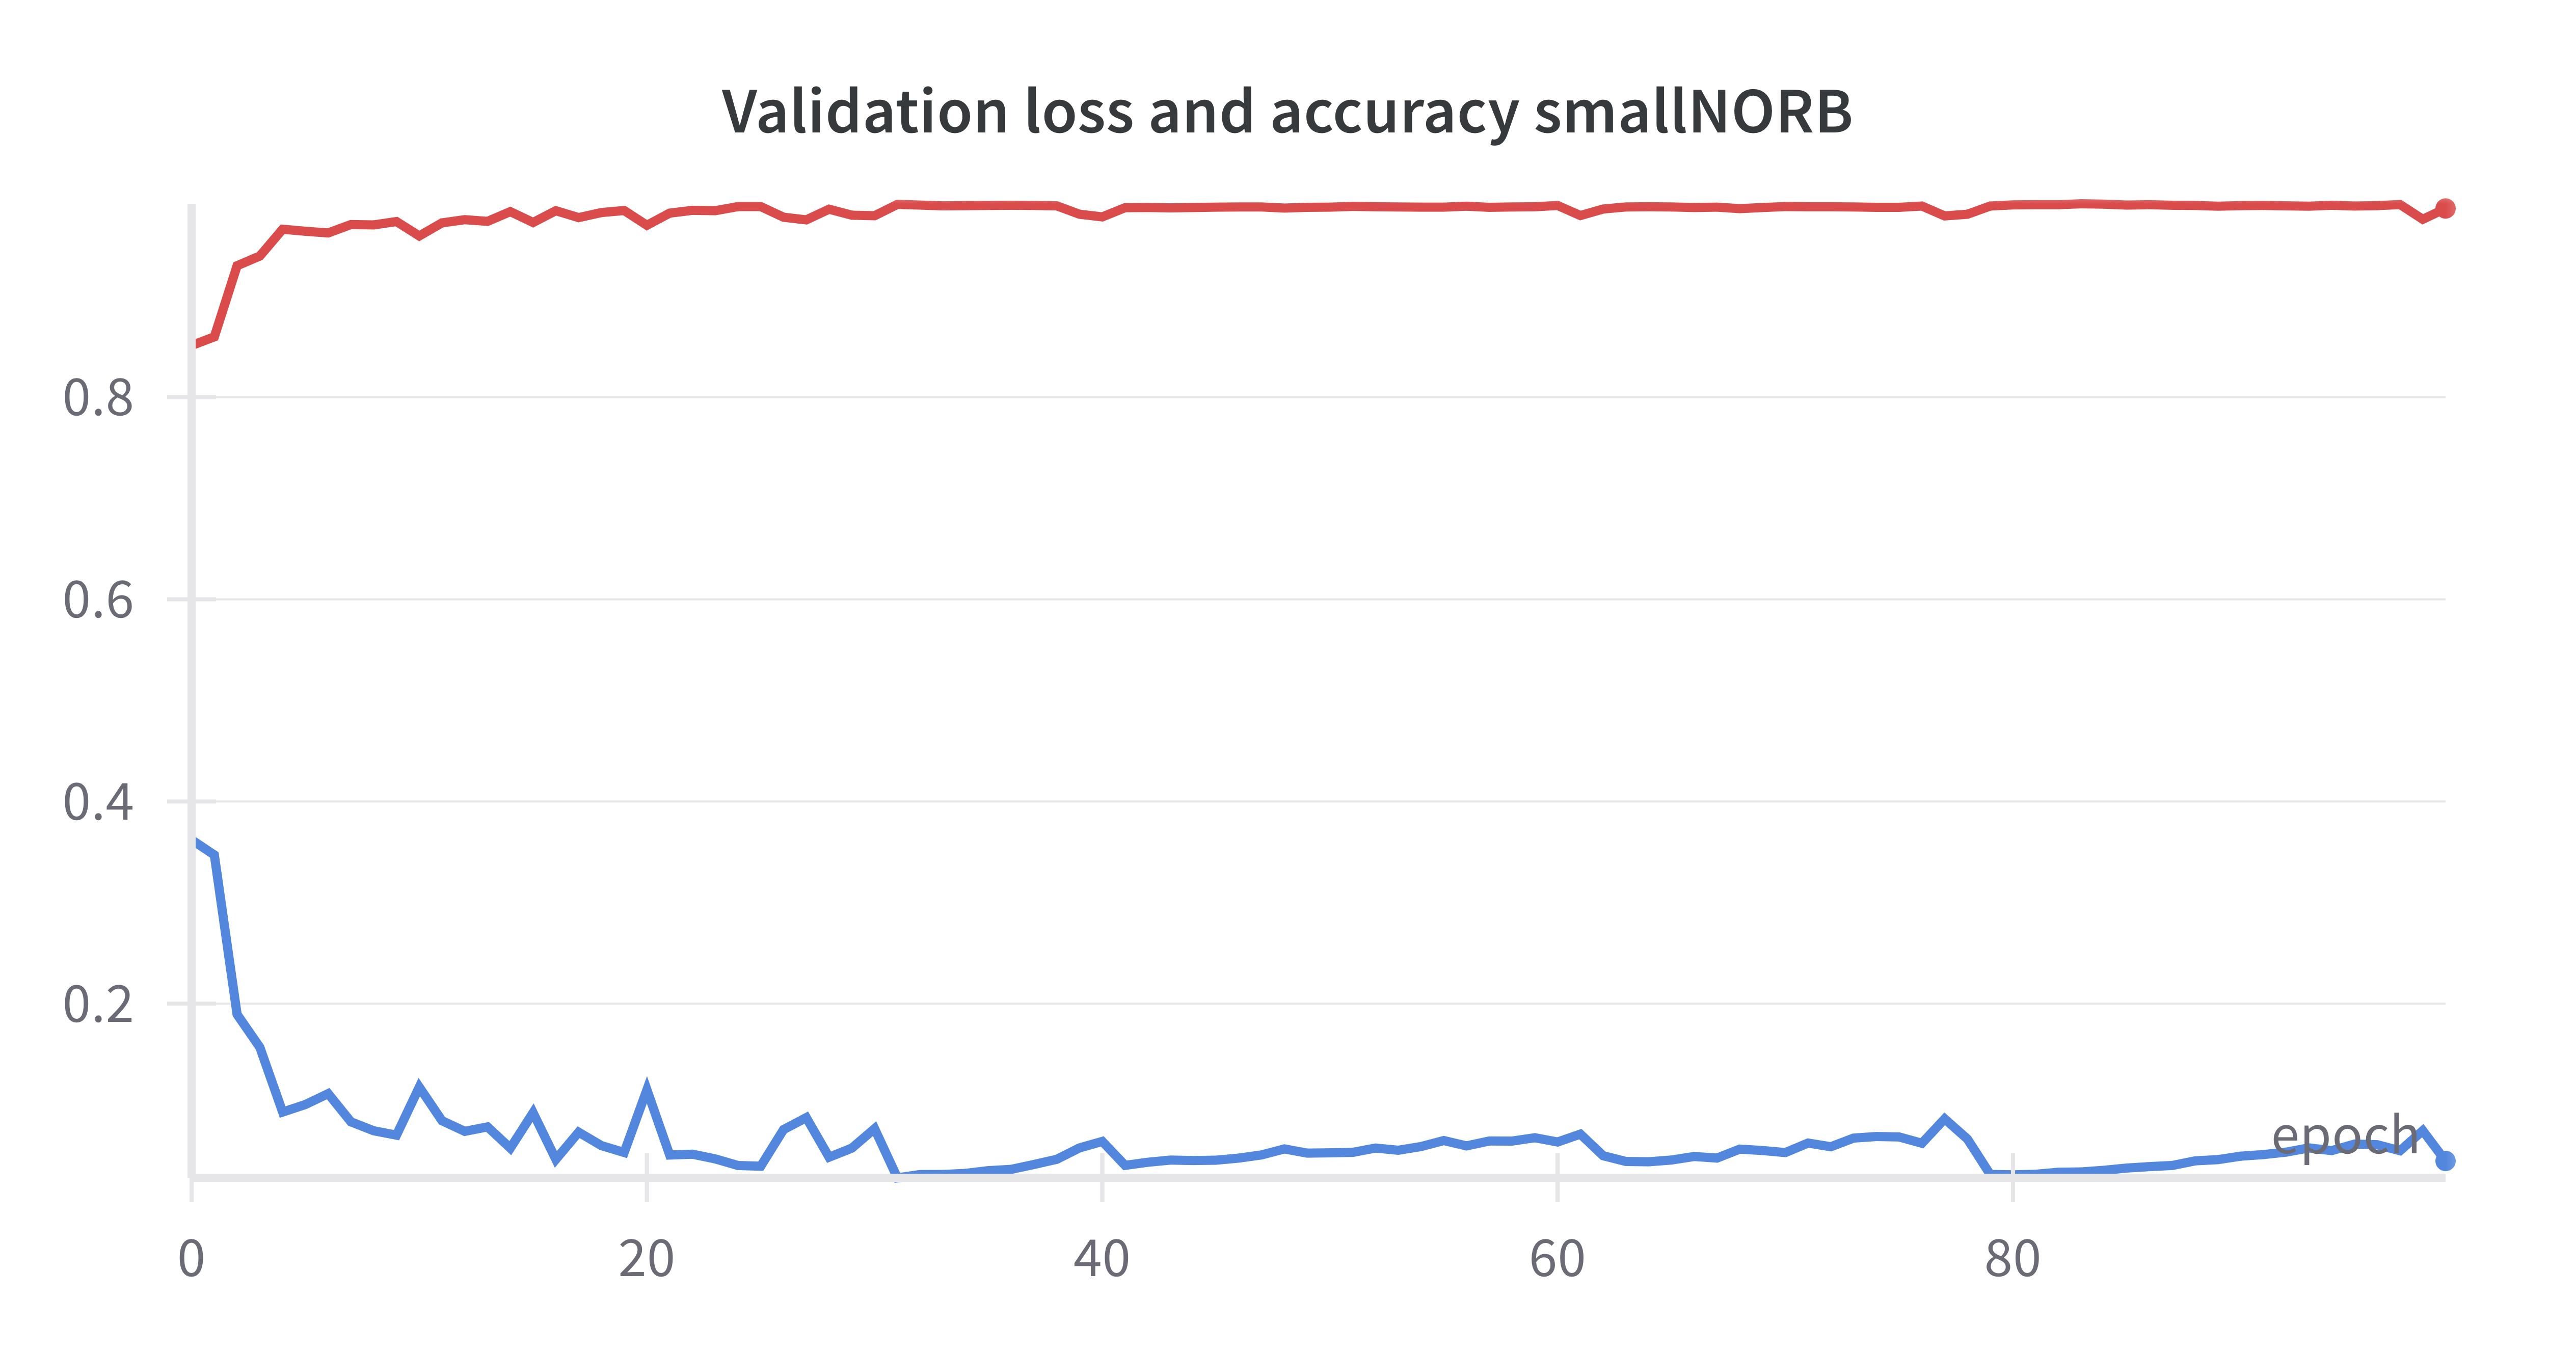
\includegraphics[width=1\linewidth]{smallnorb_val_loss_acc_mod.png}
			\caption{Validation loss/accuracy}
			\label{fig:smallnorb_val_loss_acc_mod}
		\end{subcaptionblock}%
	}
	\caption{Metriche del dataset smallNORB (con training set modificato)}
	\label{fig:smallnorb_train_val_loss_acc_mod}
\end{figure}

\noindent Di solito, un valore di accuracy che aumenta e quello di loss che non tente a diminuire, indica che il modello è in \textit{over-fitting}, cioè è in grado di memorizzare i pattern del training data e non riesce a funzionare bene con altri dati.
Un modo per risolvere questo problema è aumentare il numero di dati del training set.
Modificando il codice originale, aumentando i dati del training set a 21600 e riducendo quelli del test set a 21600, il modello sembra funzionare meglio, come possiamo vedere in figura~\ref{fig:smallnorb_train_val_loss_acc_mod}.
I risultati ottenuti sono quelli presenti nella terza riga della tabella~\ref{tab:smallnorb_val_loss_acc}.
Nel codice degli autori, oltre alla diversa divisione del dataset, il modello non ha un layer di dropout e non è presente ne la funzione di \textit{fit}, ne la configurazione dell'\textit{early stopping}.
\begin{table}[!ht]
	\centering
	\begin{tabular}[t]{|c|cc|}
		\hline
		& \textbf{Accuracy} & \textbf{Loss} \\
		\hline
		training set articolo& 0.718 & 2.001\\
		training set modificato& 0.849 & 0.445 \\
		articolo & \textbf{0.865} & - \\
		\hline
	\end{tabular}
	\caption{Test loss/accuracy smallNORB (con validation set)}
	\label{tab:smallnorb_val_loss_acc_pt}
\end{table}

\subsubsection{Codice del progetto}
Nel codice del progetto il dataset smallNORB è suddiviso come descritto nell'articolo, cioè training set: 10800, validation set: 5400 e test set: 32400).
Il risultato ottenuto è quello della prima riga della tabella~\ref{tab:smallnorb_val_loss_acc_pt}.
Come prevedibile, anche in questo caso possiamo osservare una curva anomala della validation loss simile a quella vista in precedenza (figura~\ref{fig:smallnorb_train_val_loss_acc_original_pt}).
\begin{figure}[ht]
	\centerline{% center image to the page, not to text
		\begin{subcaptionblock}{.6\textwidth}
			\centering
			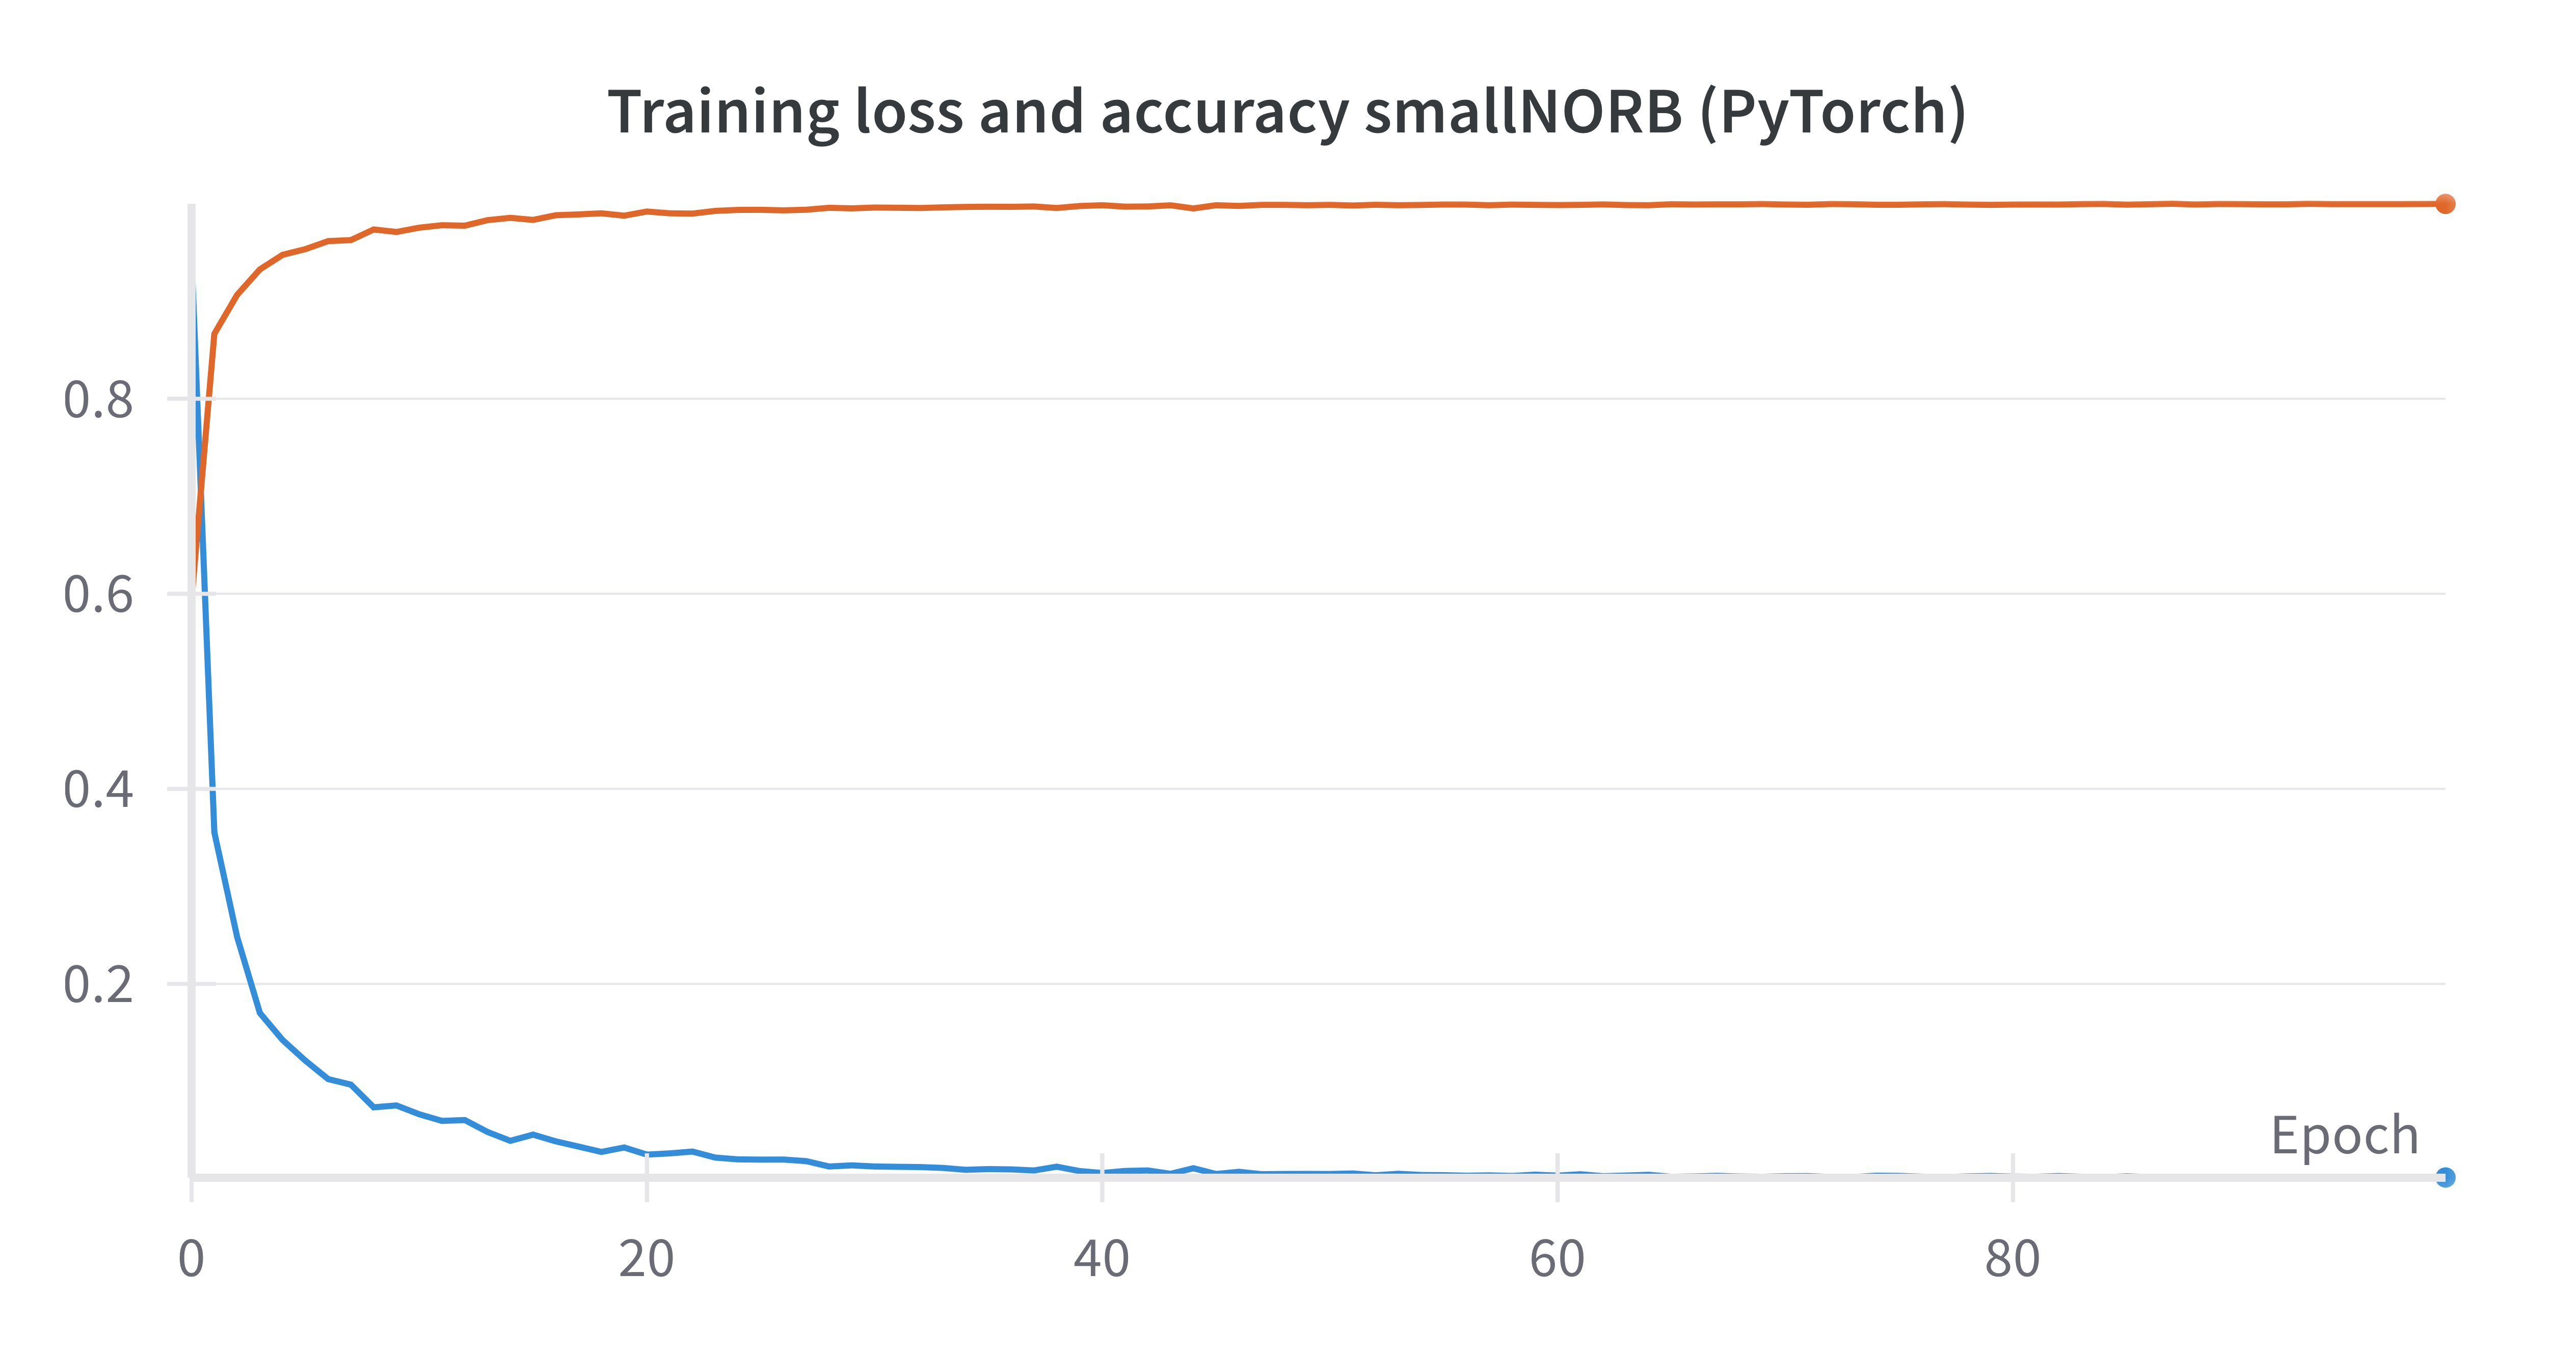
\includegraphics[width=1\linewidth]{smallnorb_train_loss_acc_original_pt.png}
			\caption{Training  loss/accuracy}
			\label{fig:smallnorb_train_loss_acc_original_pt}
		\end{subcaptionblock}%
		\begin{subcaptionblock}{.6\textwidth}
			\centering
			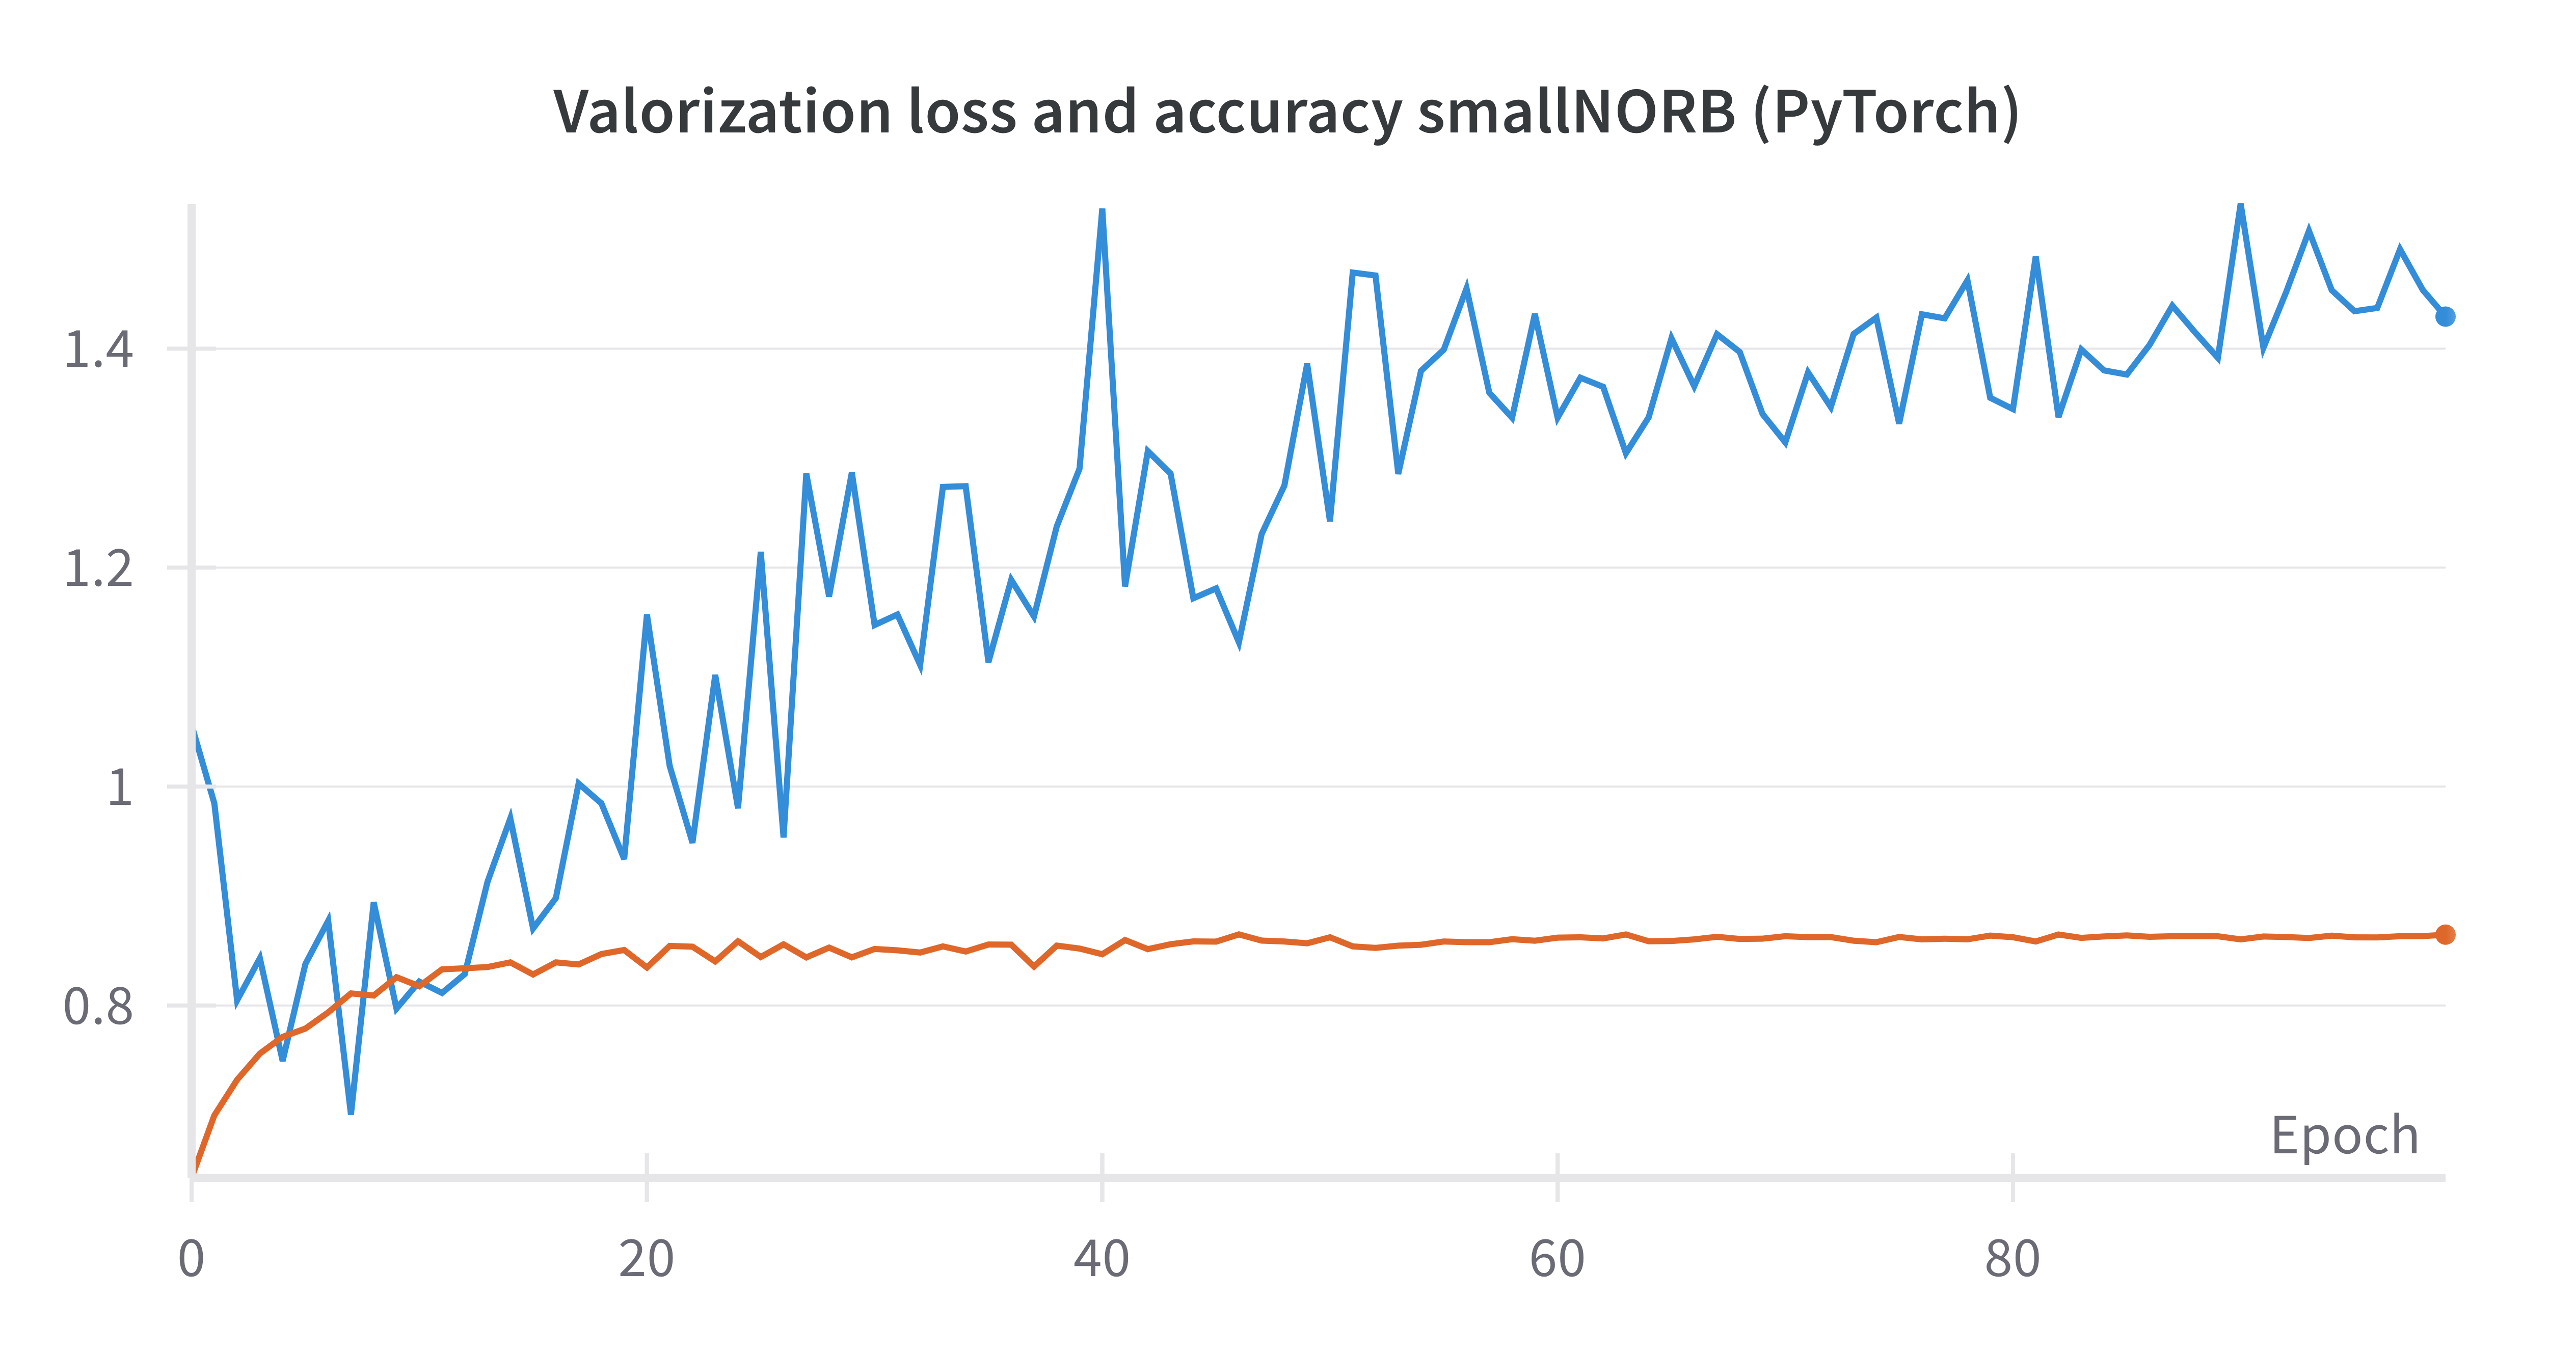
\includegraphics[width=1\linewidth]{smallnorb_val_loss_acc_original_pt.png}
			\caption{Validation loss/accuracy}
			\label{fig:smallnorb_val_loss_acc_original_pt}
		\end{subcaptionblock}%
	}
	\caption{Metriche del dataset smallNORB (con training set da articolo)}
	\label{fig:smallnorb_train_val_loss_acc_original_pt}
\end{figure}
Modificando il codice del progetto, aumentando i dati del training set a 21600 e riducendo quelli del test set a 21600, il modello sembra funzionare meglio, come possiamo vedere in figura~\ref{fig:smallnorb_train_val_loss_acc_mod_pt}.
I risultati ottenuti sono quelli presenti nella seconda riga della tabella~\ref{tab:smallnorb_val_loss_acc_pt}.

\begin{figure}[ht]
	\centerline{% center image to the page, not to text
		\begin{subcaptionblock}{.6\textwidth}
			\centering
			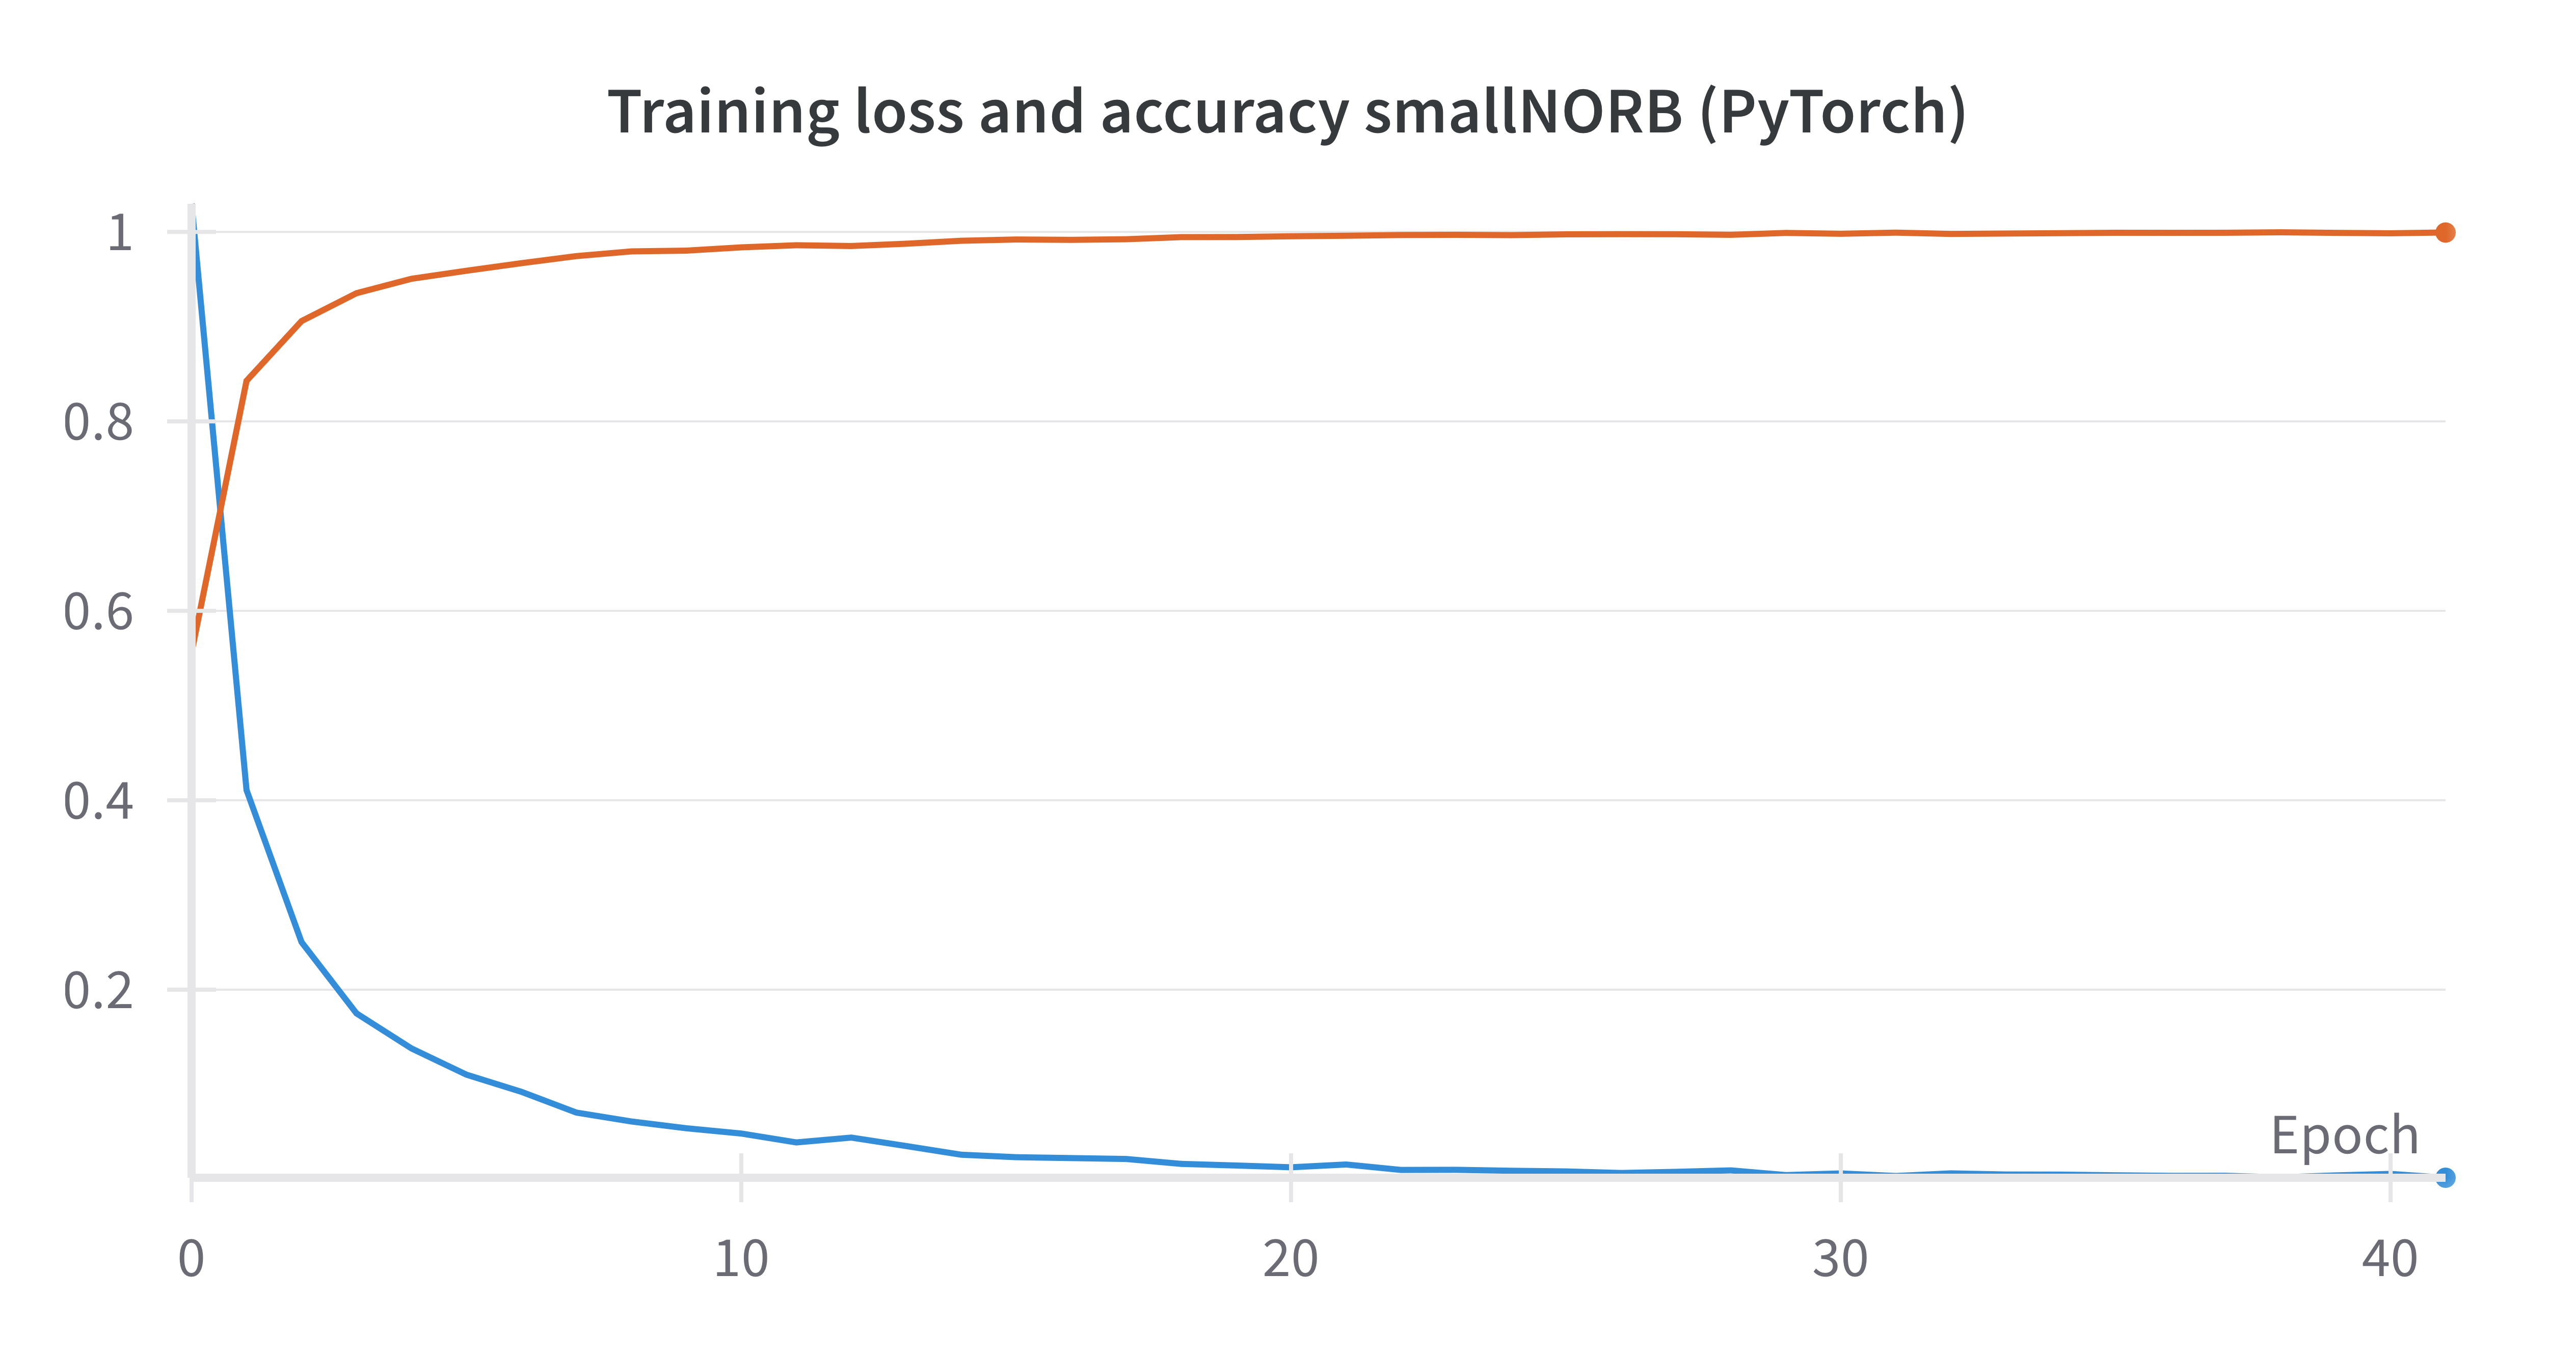
\includegraphics[width=1\linewidth]{smallnorb_train_loss_acc_mod_pt.png}
			\caption{Training  loss/accuracy}
			\label{fig:smallnorb_train_loss_acc_mod_pt.}
		\end{subcaptionblock}%
		\begin{subcaptionblock}{.6\textwidth}
			\centering
			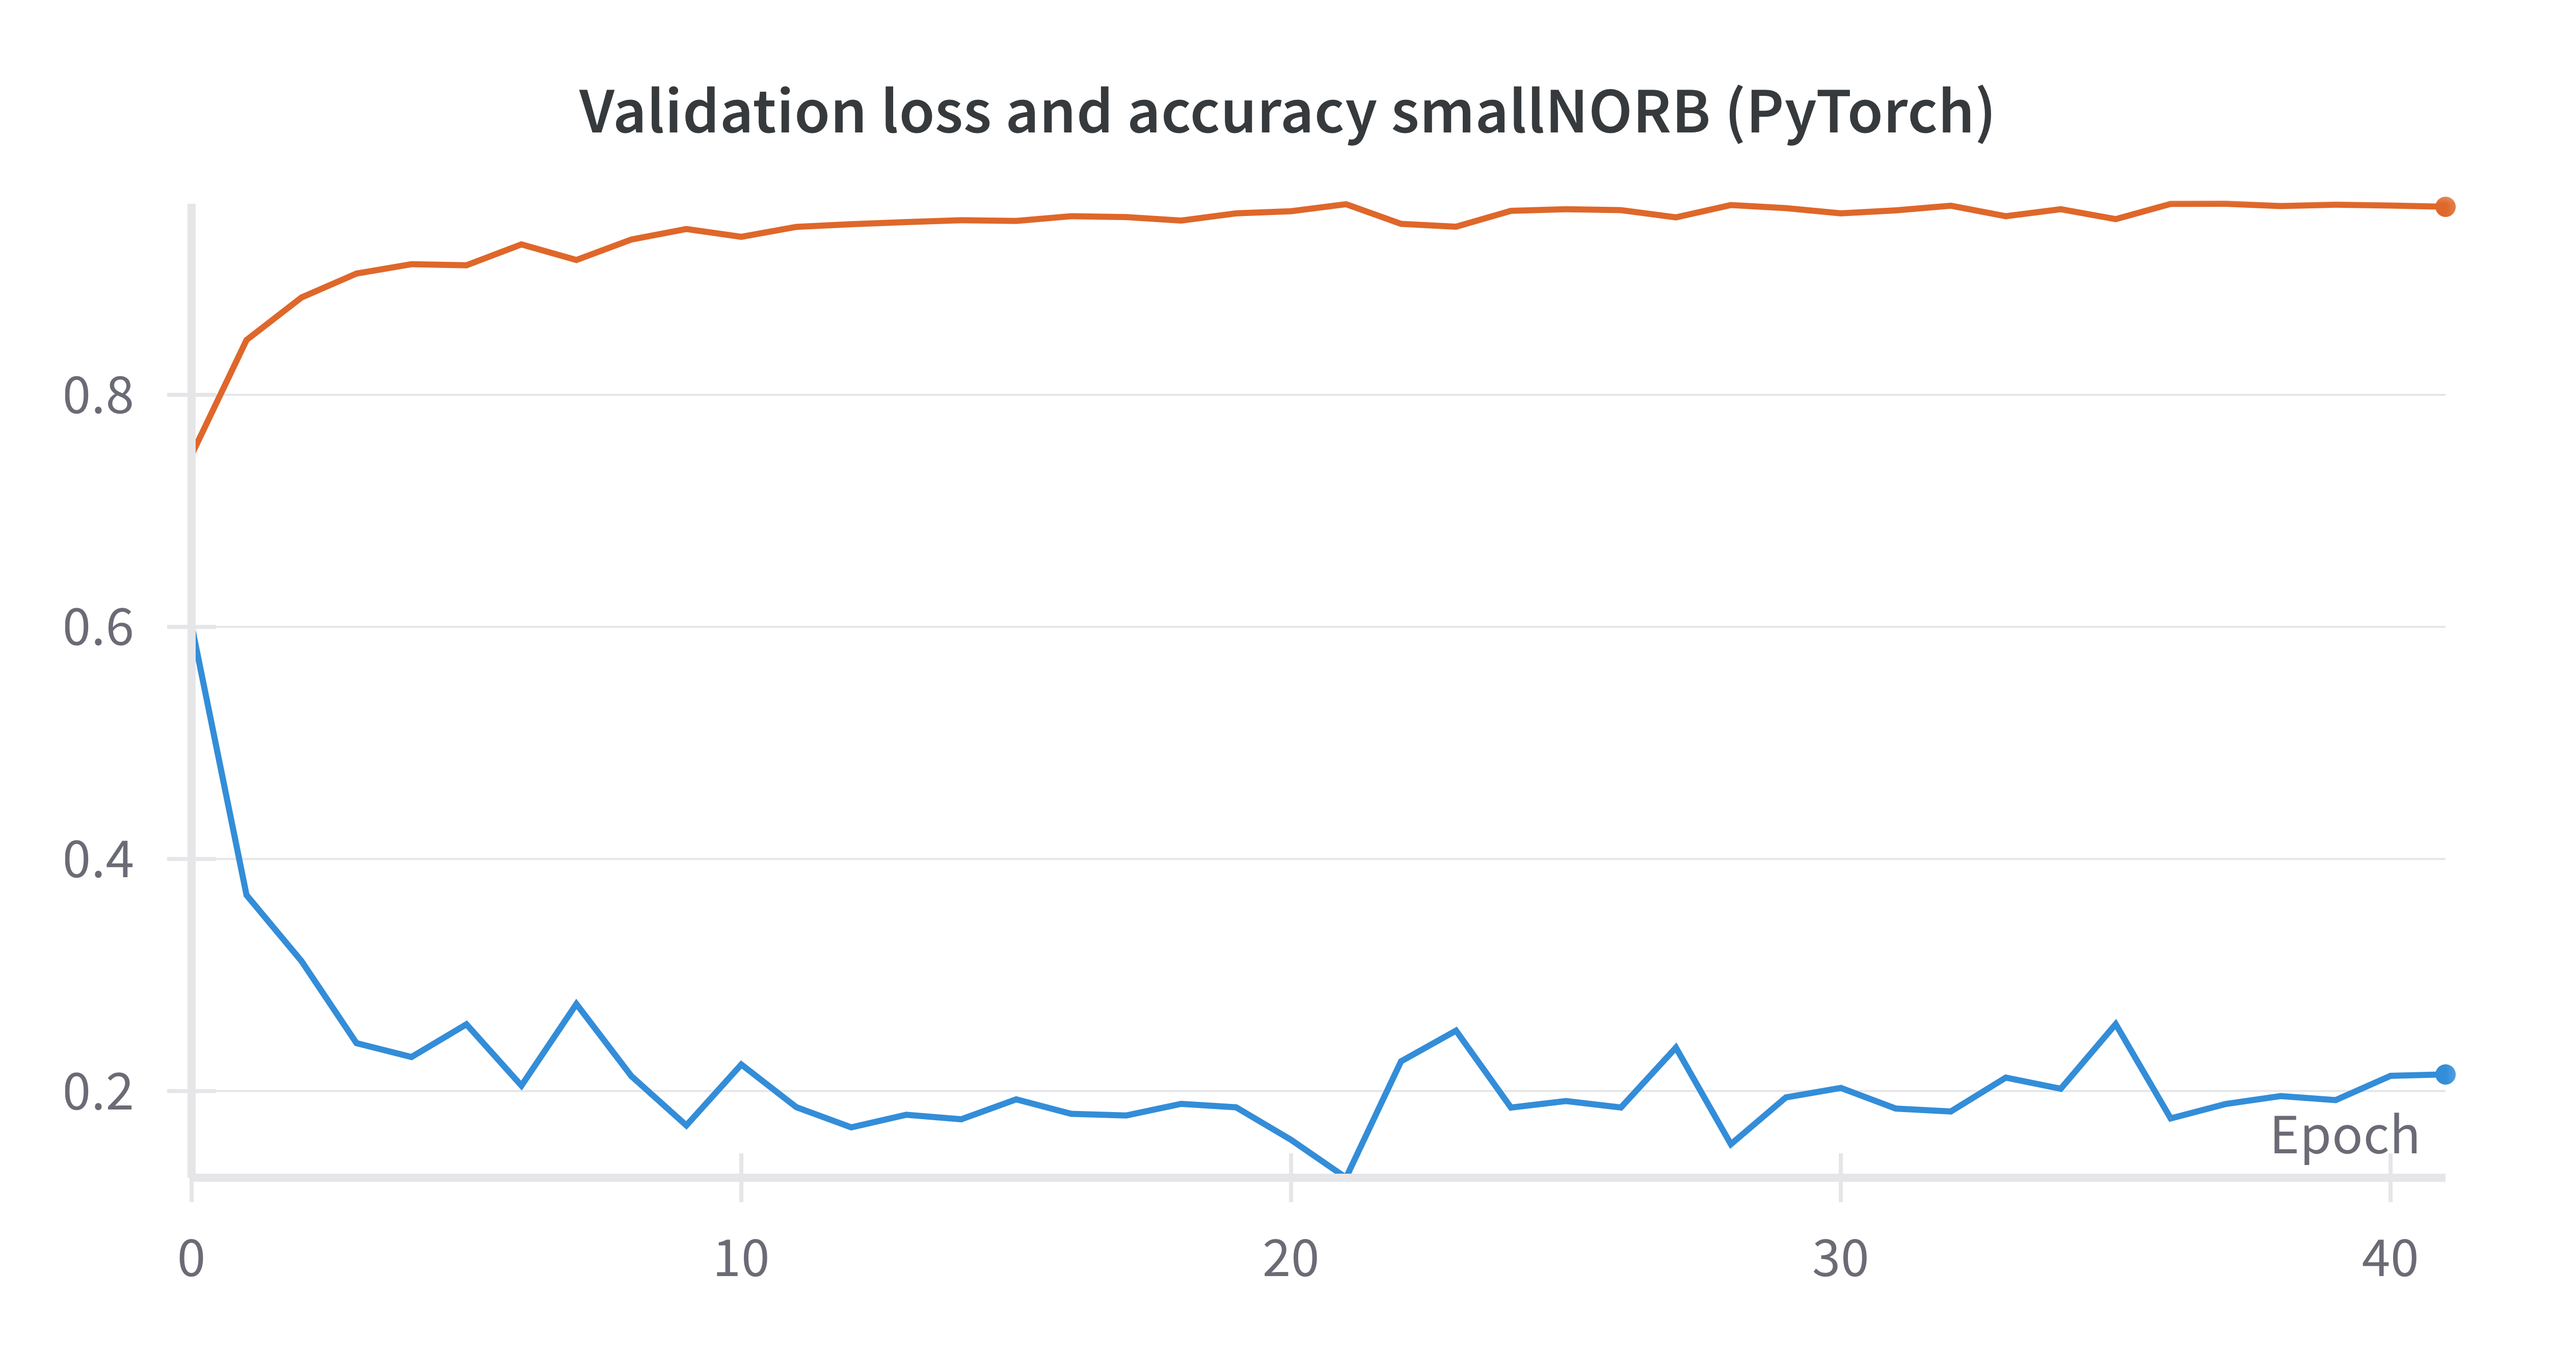
\includegraphics[width=1\linewidth]{smallnorb_val_loss_acc_mod_pt.png}
			\caption{Validation loss/accuracy}
			\label{fig:smallnorb_val_loss_acc_mod_pt.}
		\end{subcaptionblock}%
	}
	\caption{Metriche del dataset smallNORB (con training set modificato)}
	\label{fig:smallnorb_train_val_loss_acc_mod_pt}
\end{figure}


\subsection{ModelNet2D}

\subsubsection{Codice originale}
Questo dataset non è composto da immagini binoculari: per simulare la vista umana, gli autori hanno dovuto utilizzare coppie di immagini con gradi di azimut successivi.
Il codice originale presente nel repository degli autori differisce da quanto scritto nell'articolo: in particolare, la divisione del dataset non è la stessa.
Nell'articolo viene definita in questo modo:
\begin{foreigndisplaycquote}{english}[\S4.1]{neurips2019:cnn2}
On the ModelNet2D dataset, we use the images taken from azimuths of degrees from 50 to 125 as the training set, degrees from 30 to 45 and from 130 to 145 as the validation set, and unlimited degrees as the test set.
\end{foreigndisplaycquote}
mentre nel codice originale il dataset è diviso in base all'angolazione: da 30 a 40 gradi per il training set, da 45 a 50 per il validation set e da 55 a 70 per il test set.
\begin{table}[!ht]
	\centering
	\begin{tabular}[t]{|c|cc|}
		\hline
		& \textbf{Accuracy} & \textbf{Loss} \\
		\hline
		training set articolo& 0.859 & 0.462 \\
		training set maggiore& 0.912 & 0.874 \\
		articolo & \textbf{0.941} & - \\
		\hline
	\end{tabular}
	\caption{Test loss/accuracy ModelNet2D}
	\label{tab:modelnet2d_val_loss_acc_pt}
\end{table}
Nell'articolo gli autori scrivono di aver fatto il render dei modelli CAD degli oggetti a partire da un angolazione di 30 gradi: osservando le immagini in figura~\ref{fig:modelnet2d_samples}, sembra che l'angolazione sia inferiore a quelle dichiarata.
Oltre alla diversa divisione del dataset, il modello non ha un layer di dropout e non è presente ne la funzione di \textit{fit}, ne la configurazione dell'\textit{early stopping}.

\subsubsection{Codice del progetto}
\noindent Utilizzando la suddivisione del dataset presente nell'articolo (training set: 5400, test set: 16200 e validation set: 2700), il risultato è quello nella prima riga della tabella~\ref{tab:modelnet2d_val_loss_acc_pt}, inferiore a quanto ottenuto dagli autori.
\begin{figure}[!ht]
	\centerline{% center image to the page, not to text
		\begin{subcaptionblock}{0.6\textwidth}
			\centering
			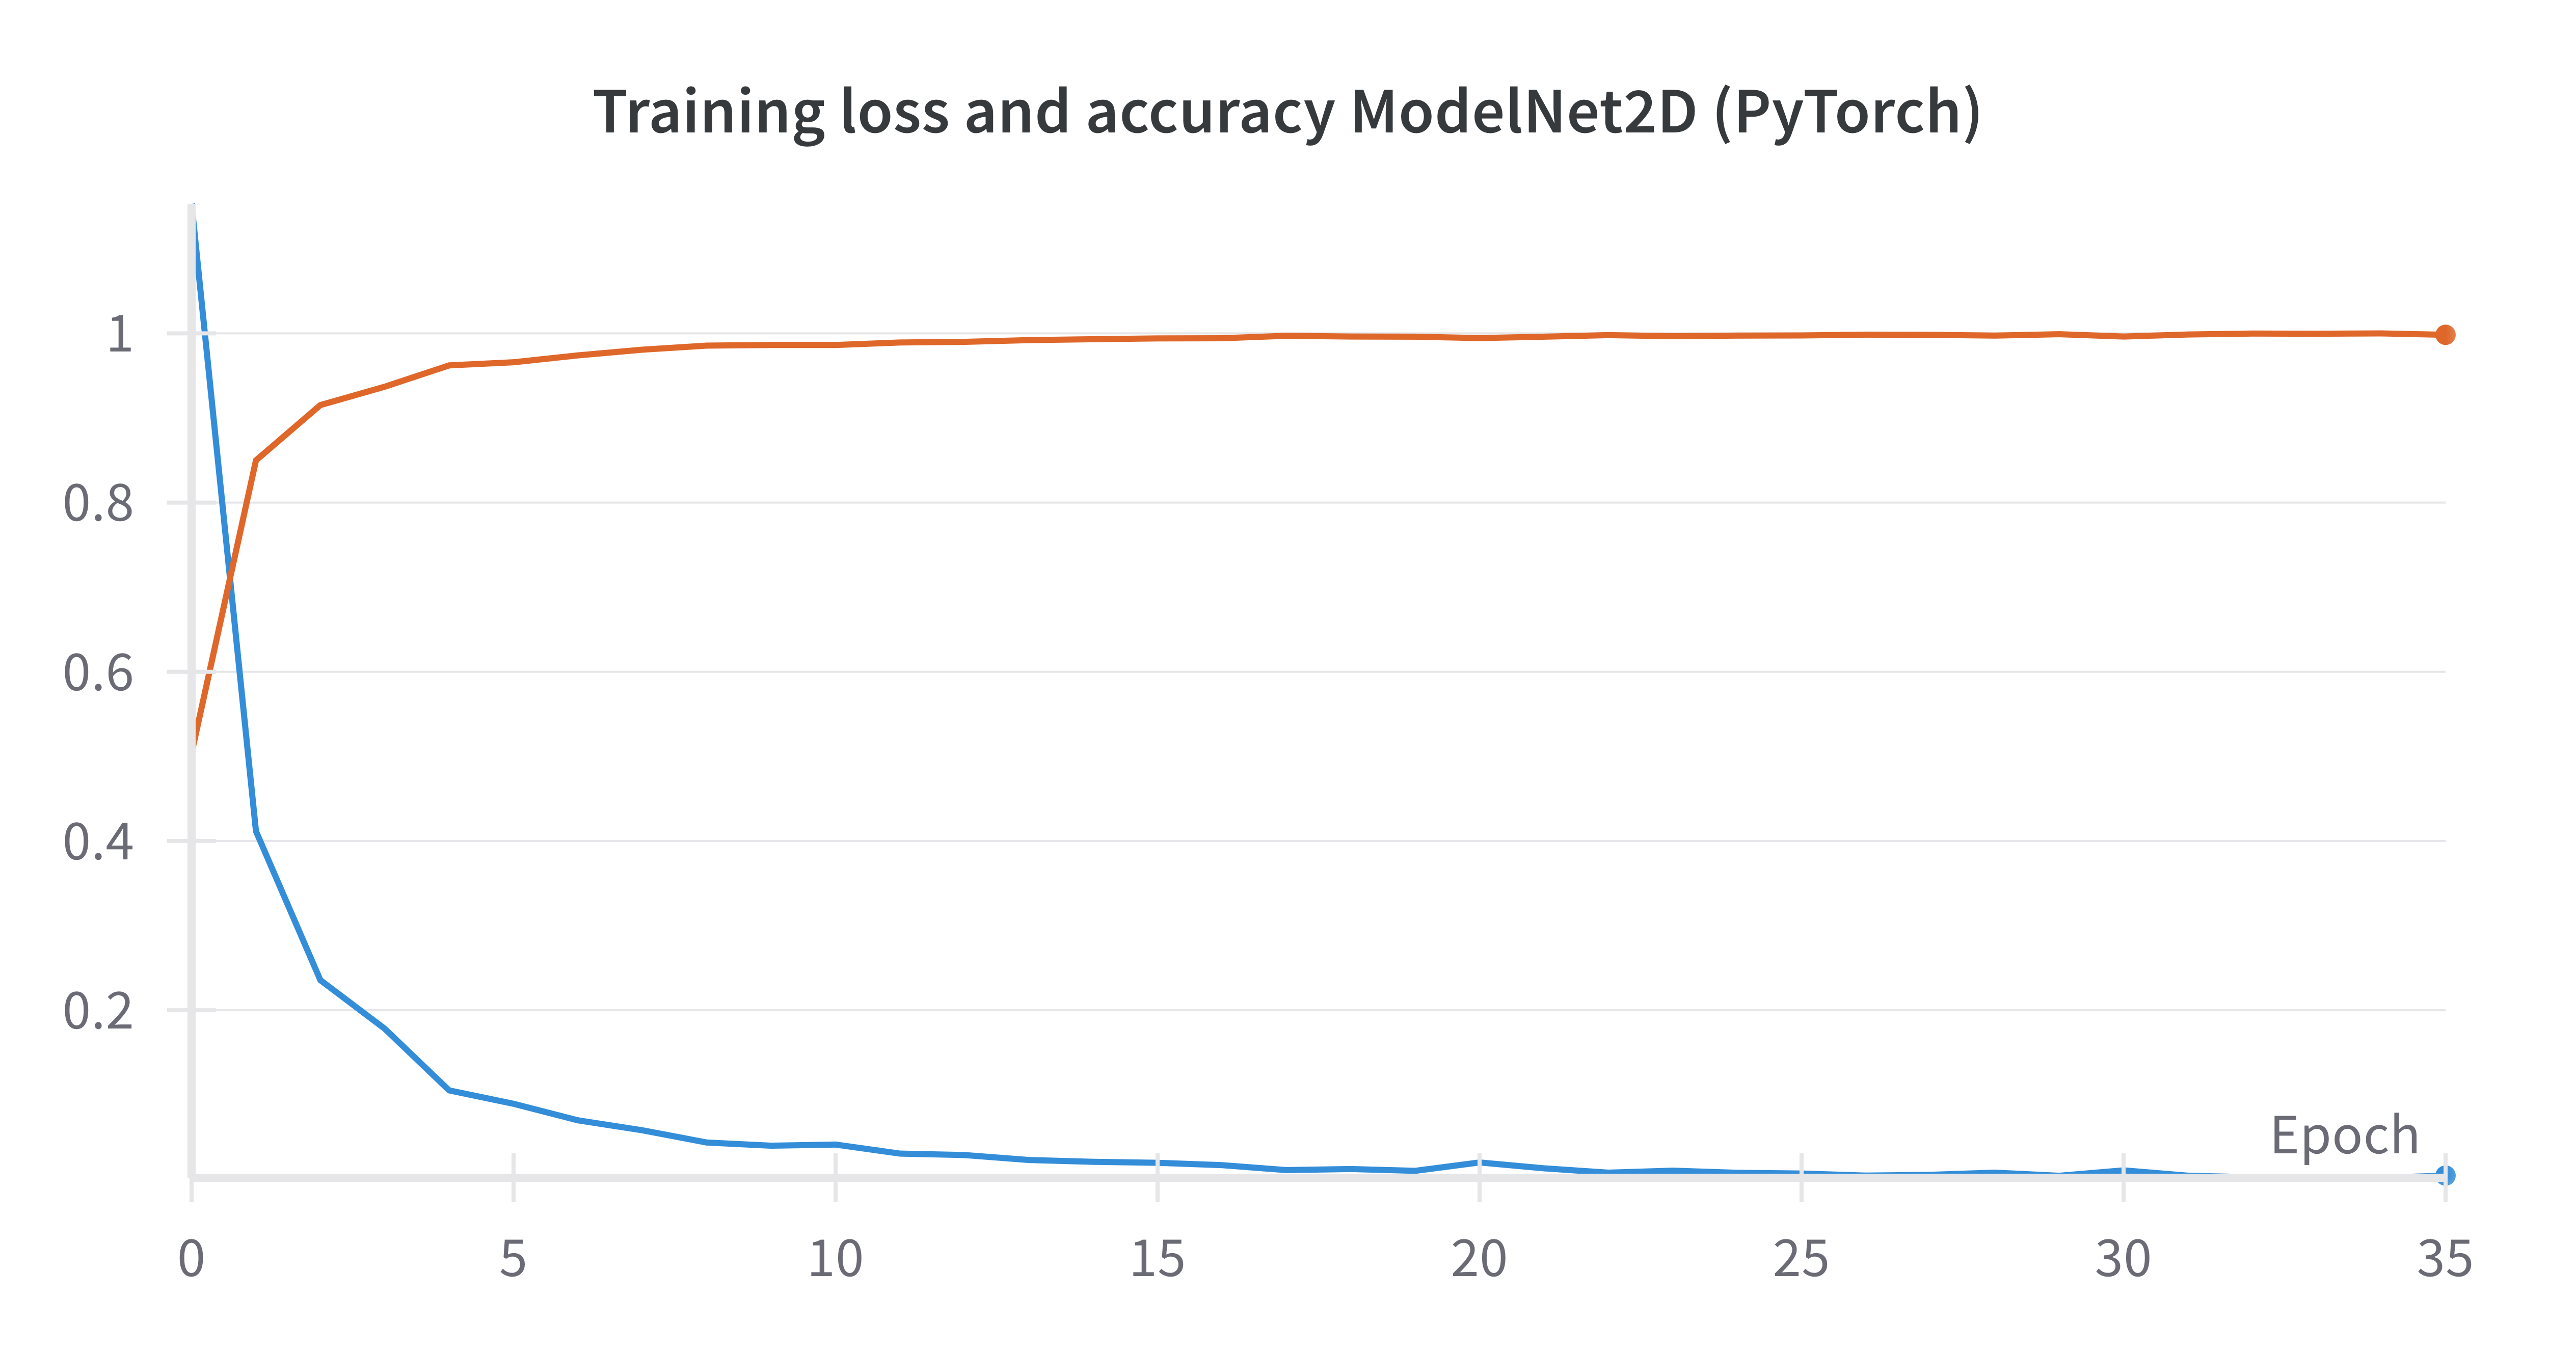
\includegraphics[width=0.9\linewidth]{modelnet_train_loss_acc_original_pt.png}
			\caption{Training  loss/accuracy}
			\label{fig:modelnet2d_train_loss_acc_original_pt}
		\end{subcaptionblock}%
		\begin{subcaptionblock}{0.6\textwidth}
			\centering
			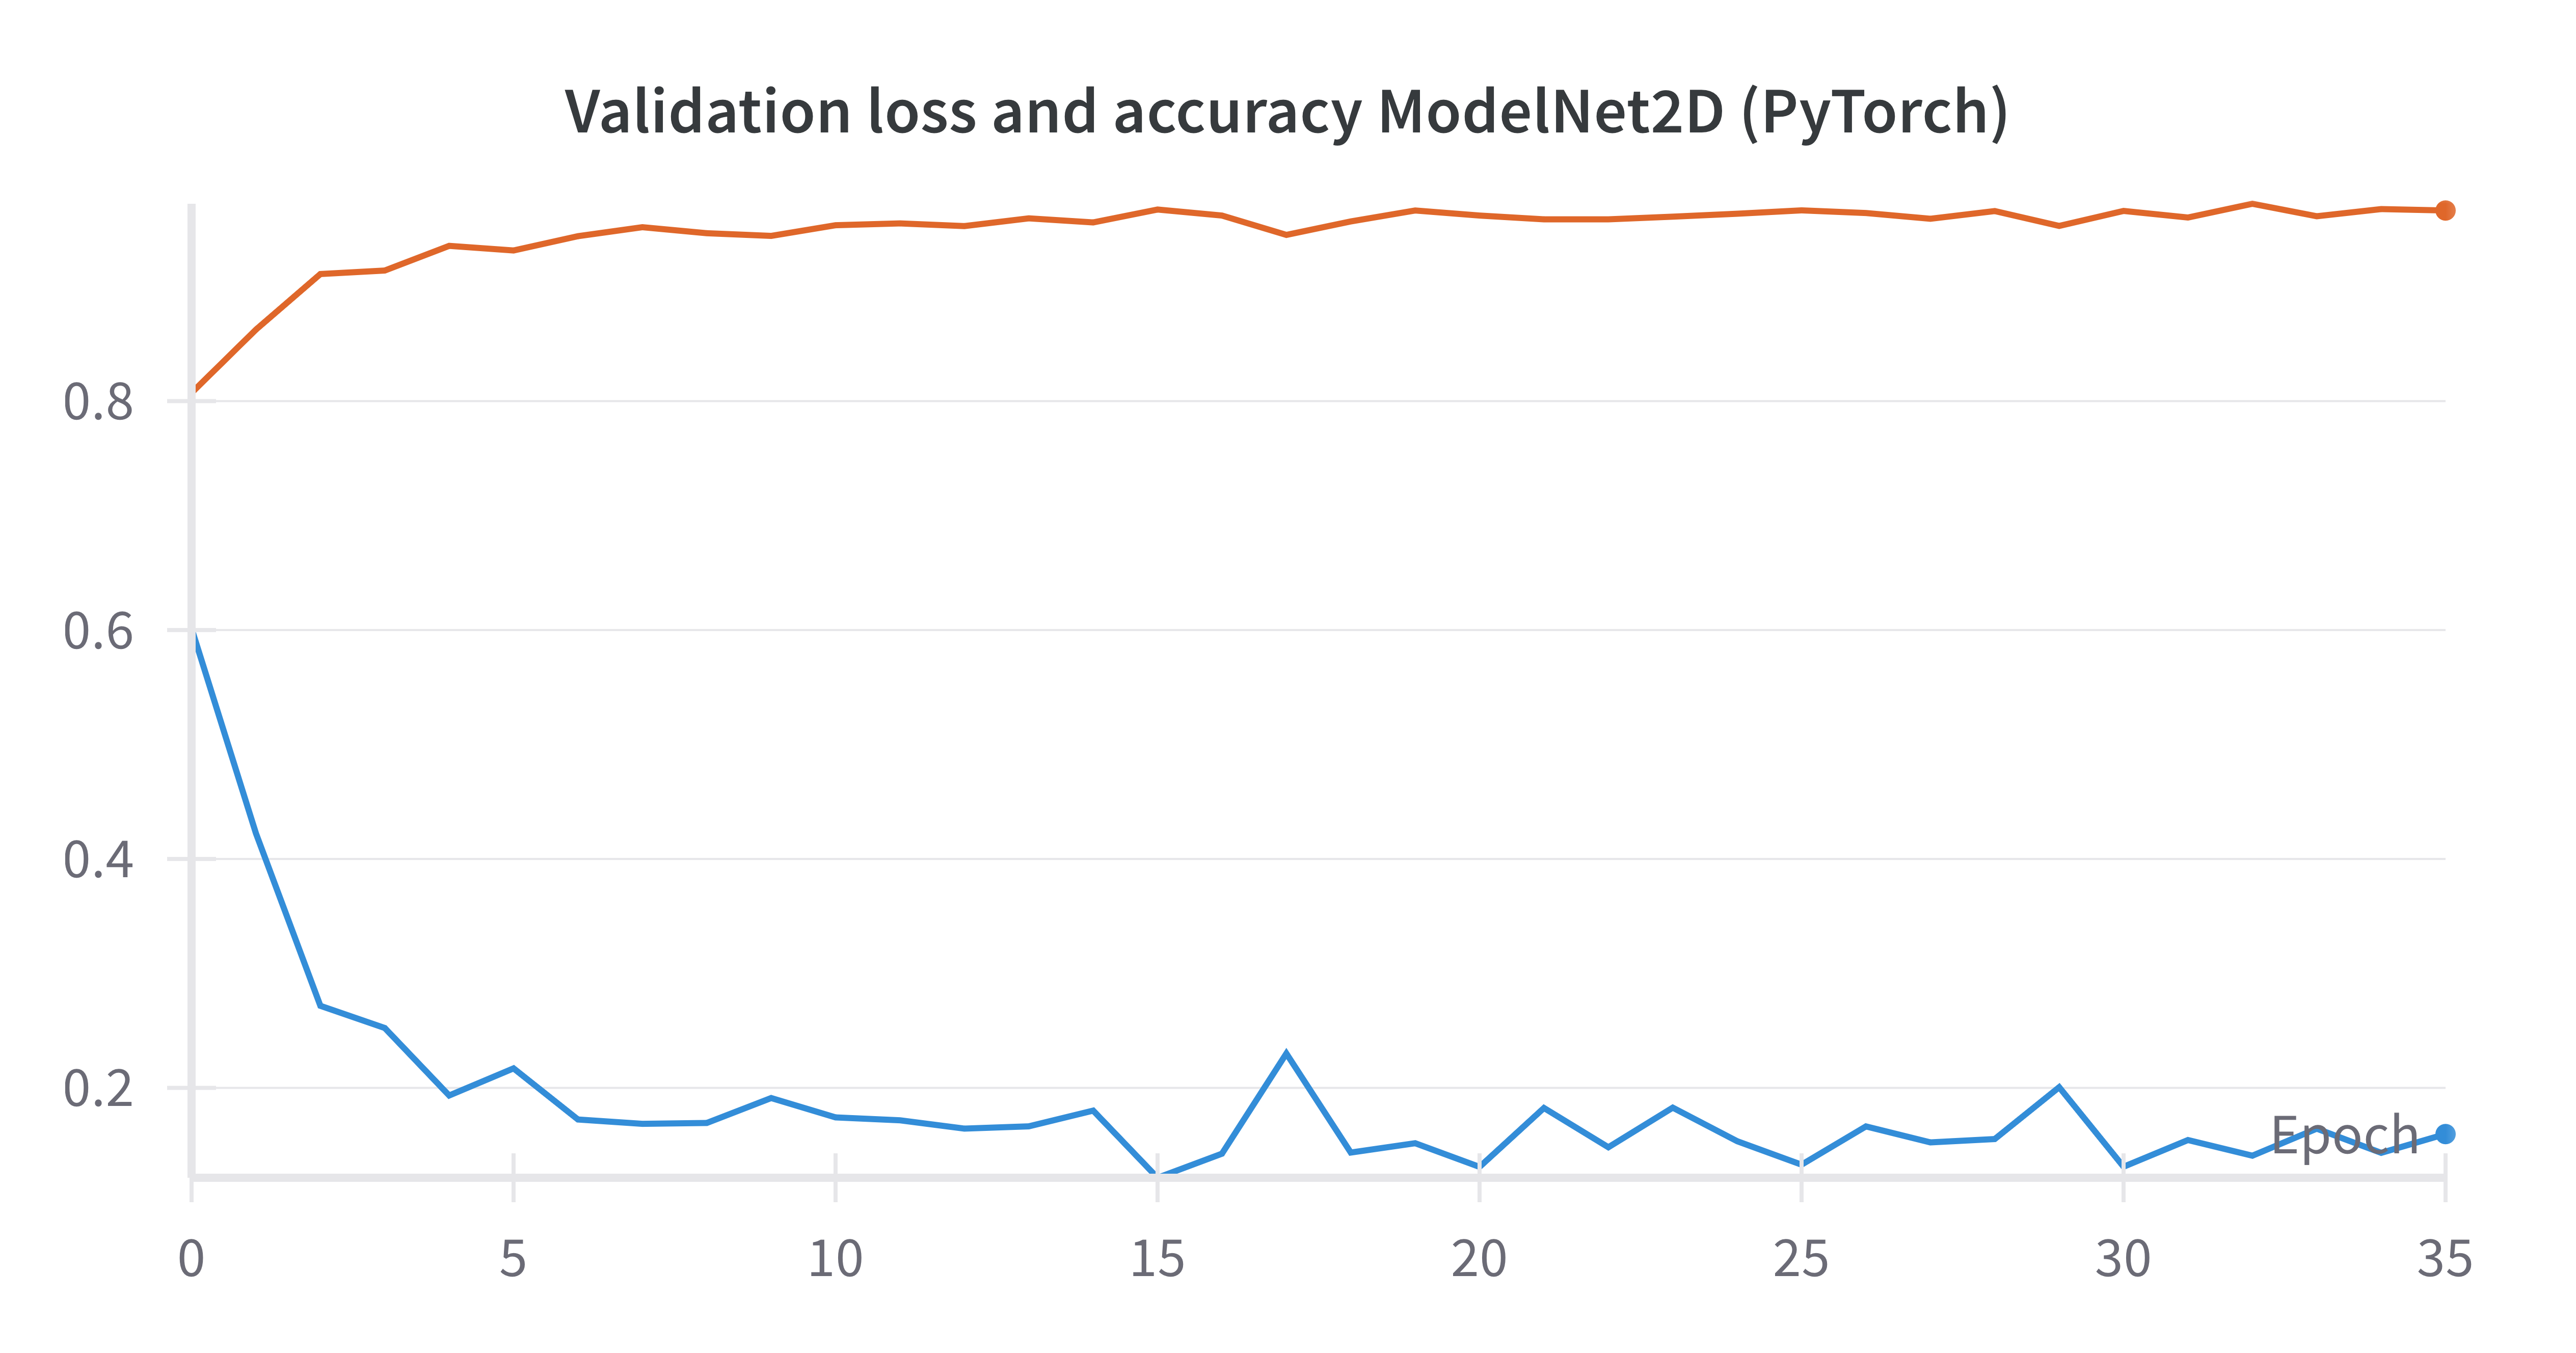
\includegraphics[width=0.9\linewidth]{modelnet_val_loss_acc_original_pt.png}
			\caption{Validation loss/accuracy}
			\label{fig:modelnet2d_val_loss_acc_original_pt}
		\end{subcaptionblock}%
	}
	\caption{Metriche del dataset ModelNet2D}
	\label{fig:modelnet2d_train_val_loss_acc_original_pt}
\end{figure}
Con quella suddivisione possiamo osservare, in figura~\ref{fig:modelnet2d_train_val_loss_acc_original_pt}, come la curva della validation loss non presenti anomalie.
Modificando il codice del progetto, come fatto in precedenza, cioè aumentando i dati del training set a 10800 e riducendo quelli del test set a 10800, il modello sembra funzionare meglio, come possiamo vedere in figura~\ref{fig:modelnet2d_train_val_loss_acc_mod_pt}.
I risultati ottenuti sono quelli presenti nella seconda riga della tabella~\ref{tab:modelnet2d_val_loss_acc_pt}.

\begin{figure}[!ht]
	\centerline{% center image to the page, not to text
		\begin{subcaptionblock}{0.6\textwidth}
			\centering
			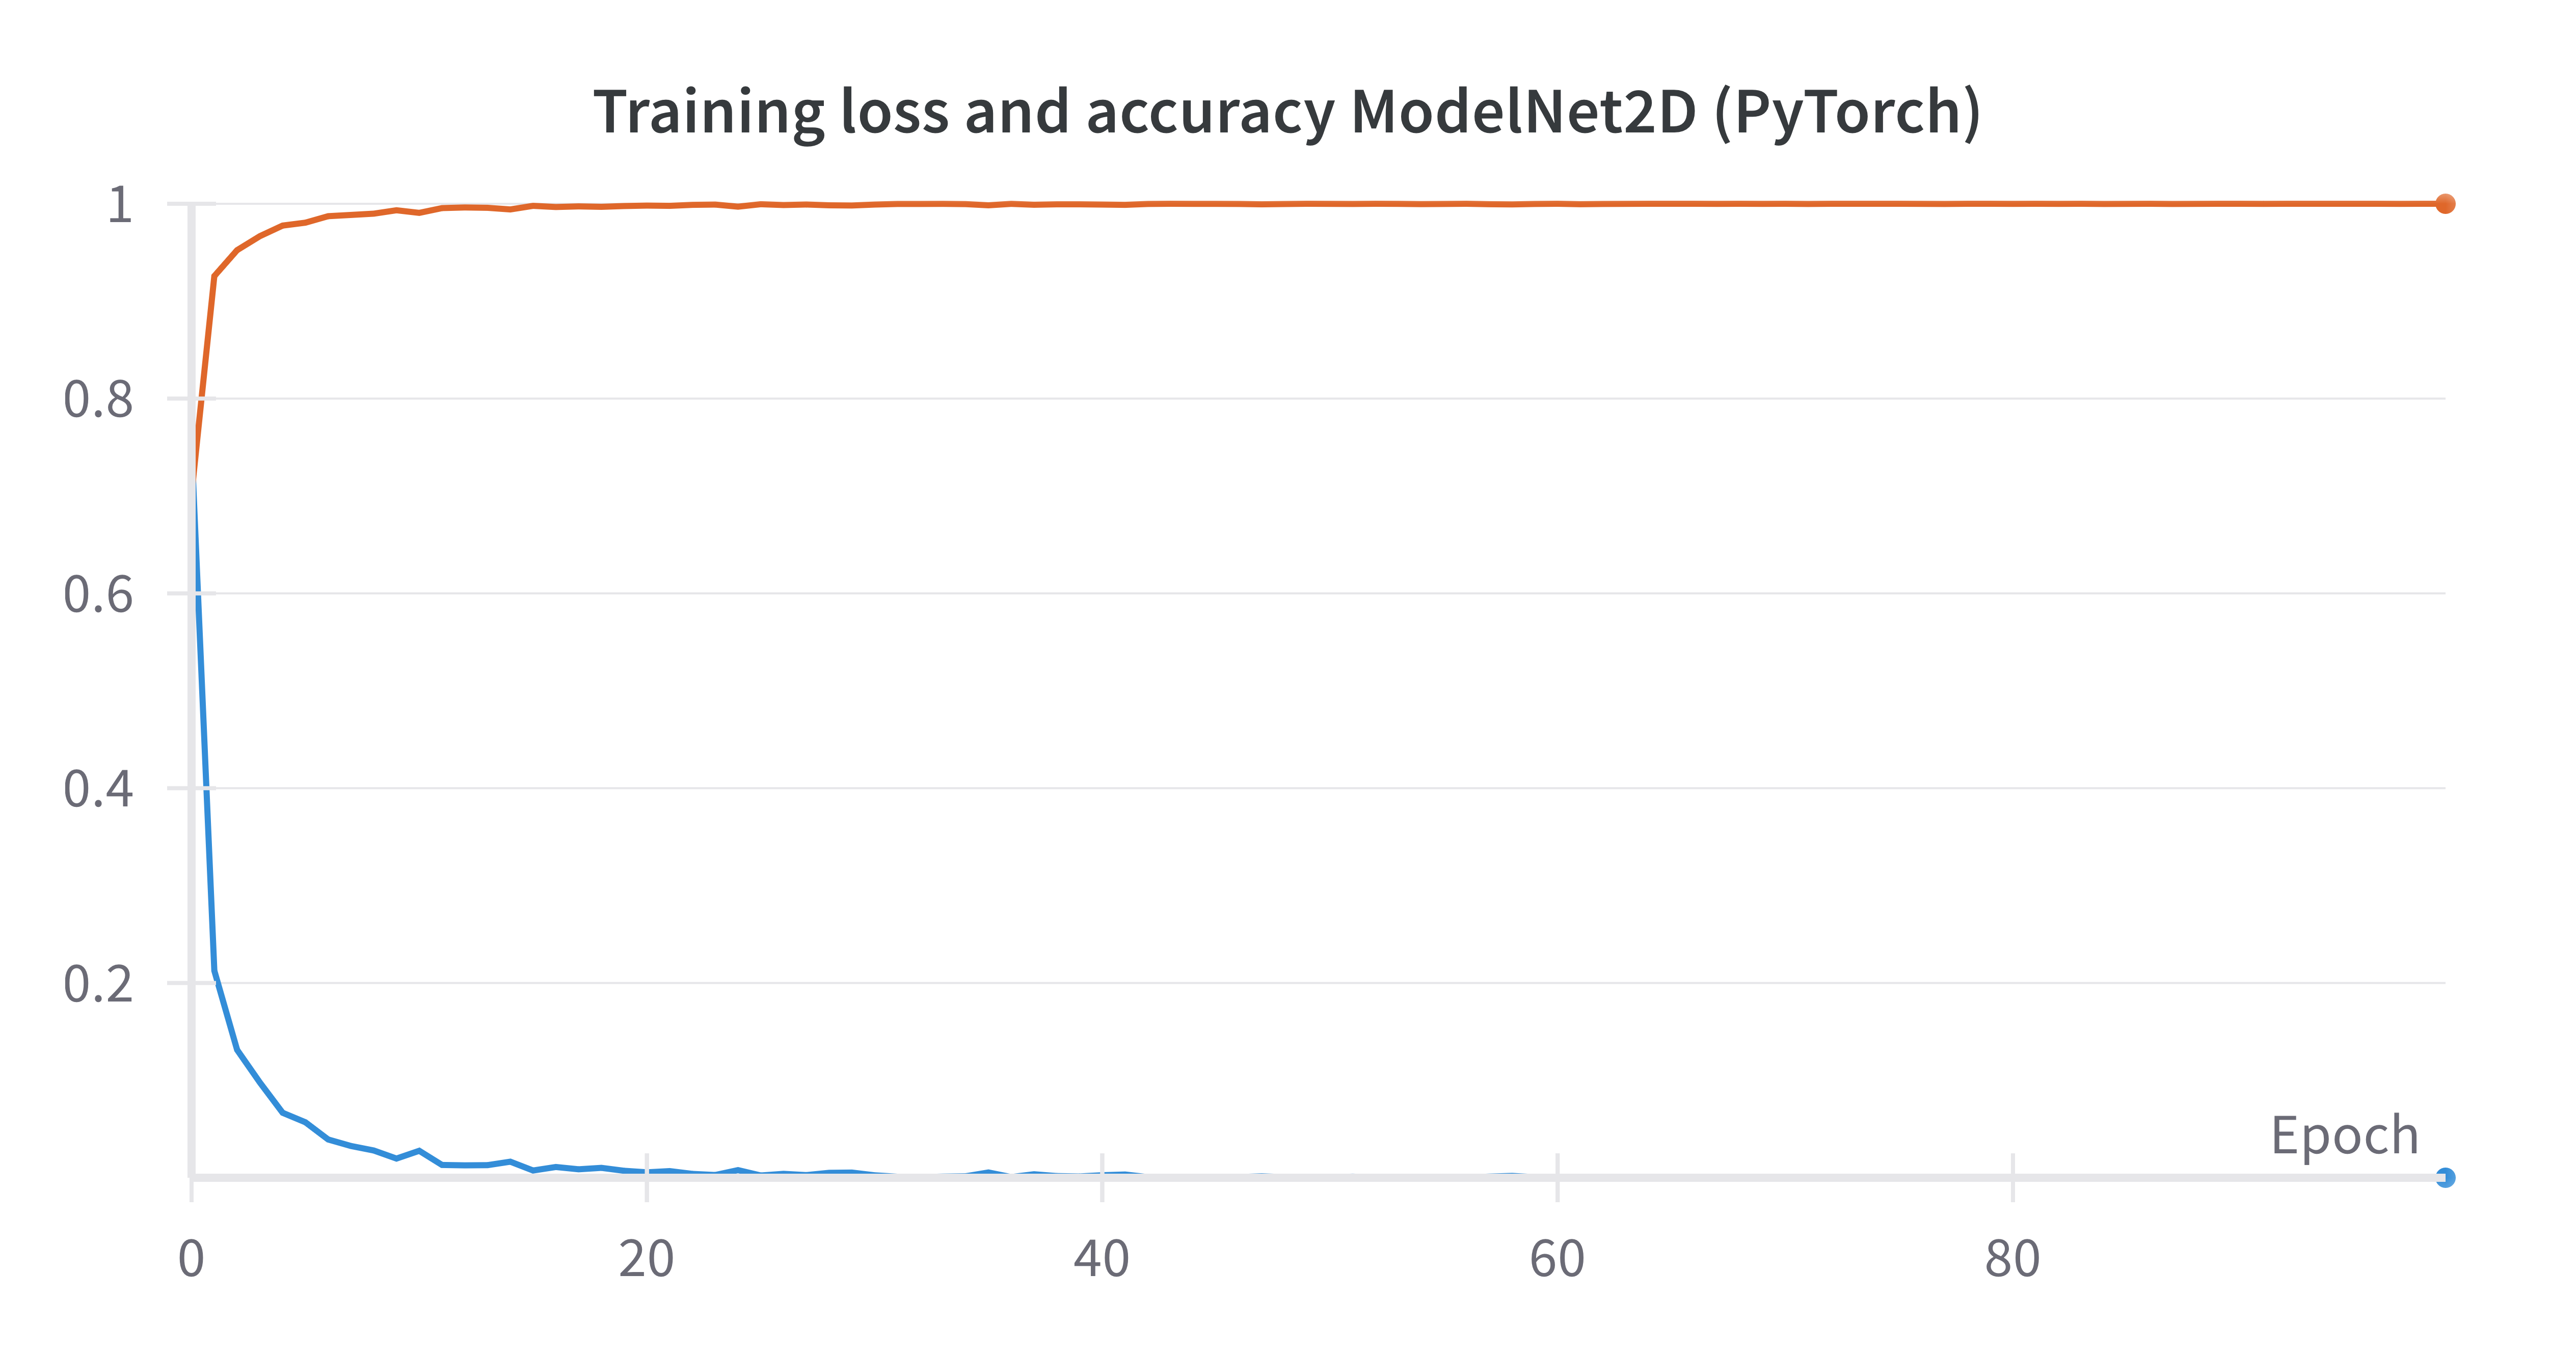
\includegraphics[width=1\linewidth]{modelnet_train_loss_acc_mod_pt.png}
			\caption{Training  loss/accuracy}
			\label{fig:modelnet2d_train_loss_acc_mod_pt}
		\end{subcaptionblock}%
		\begin{subcaptionblock}{0.6\textwidth}
			\centering
			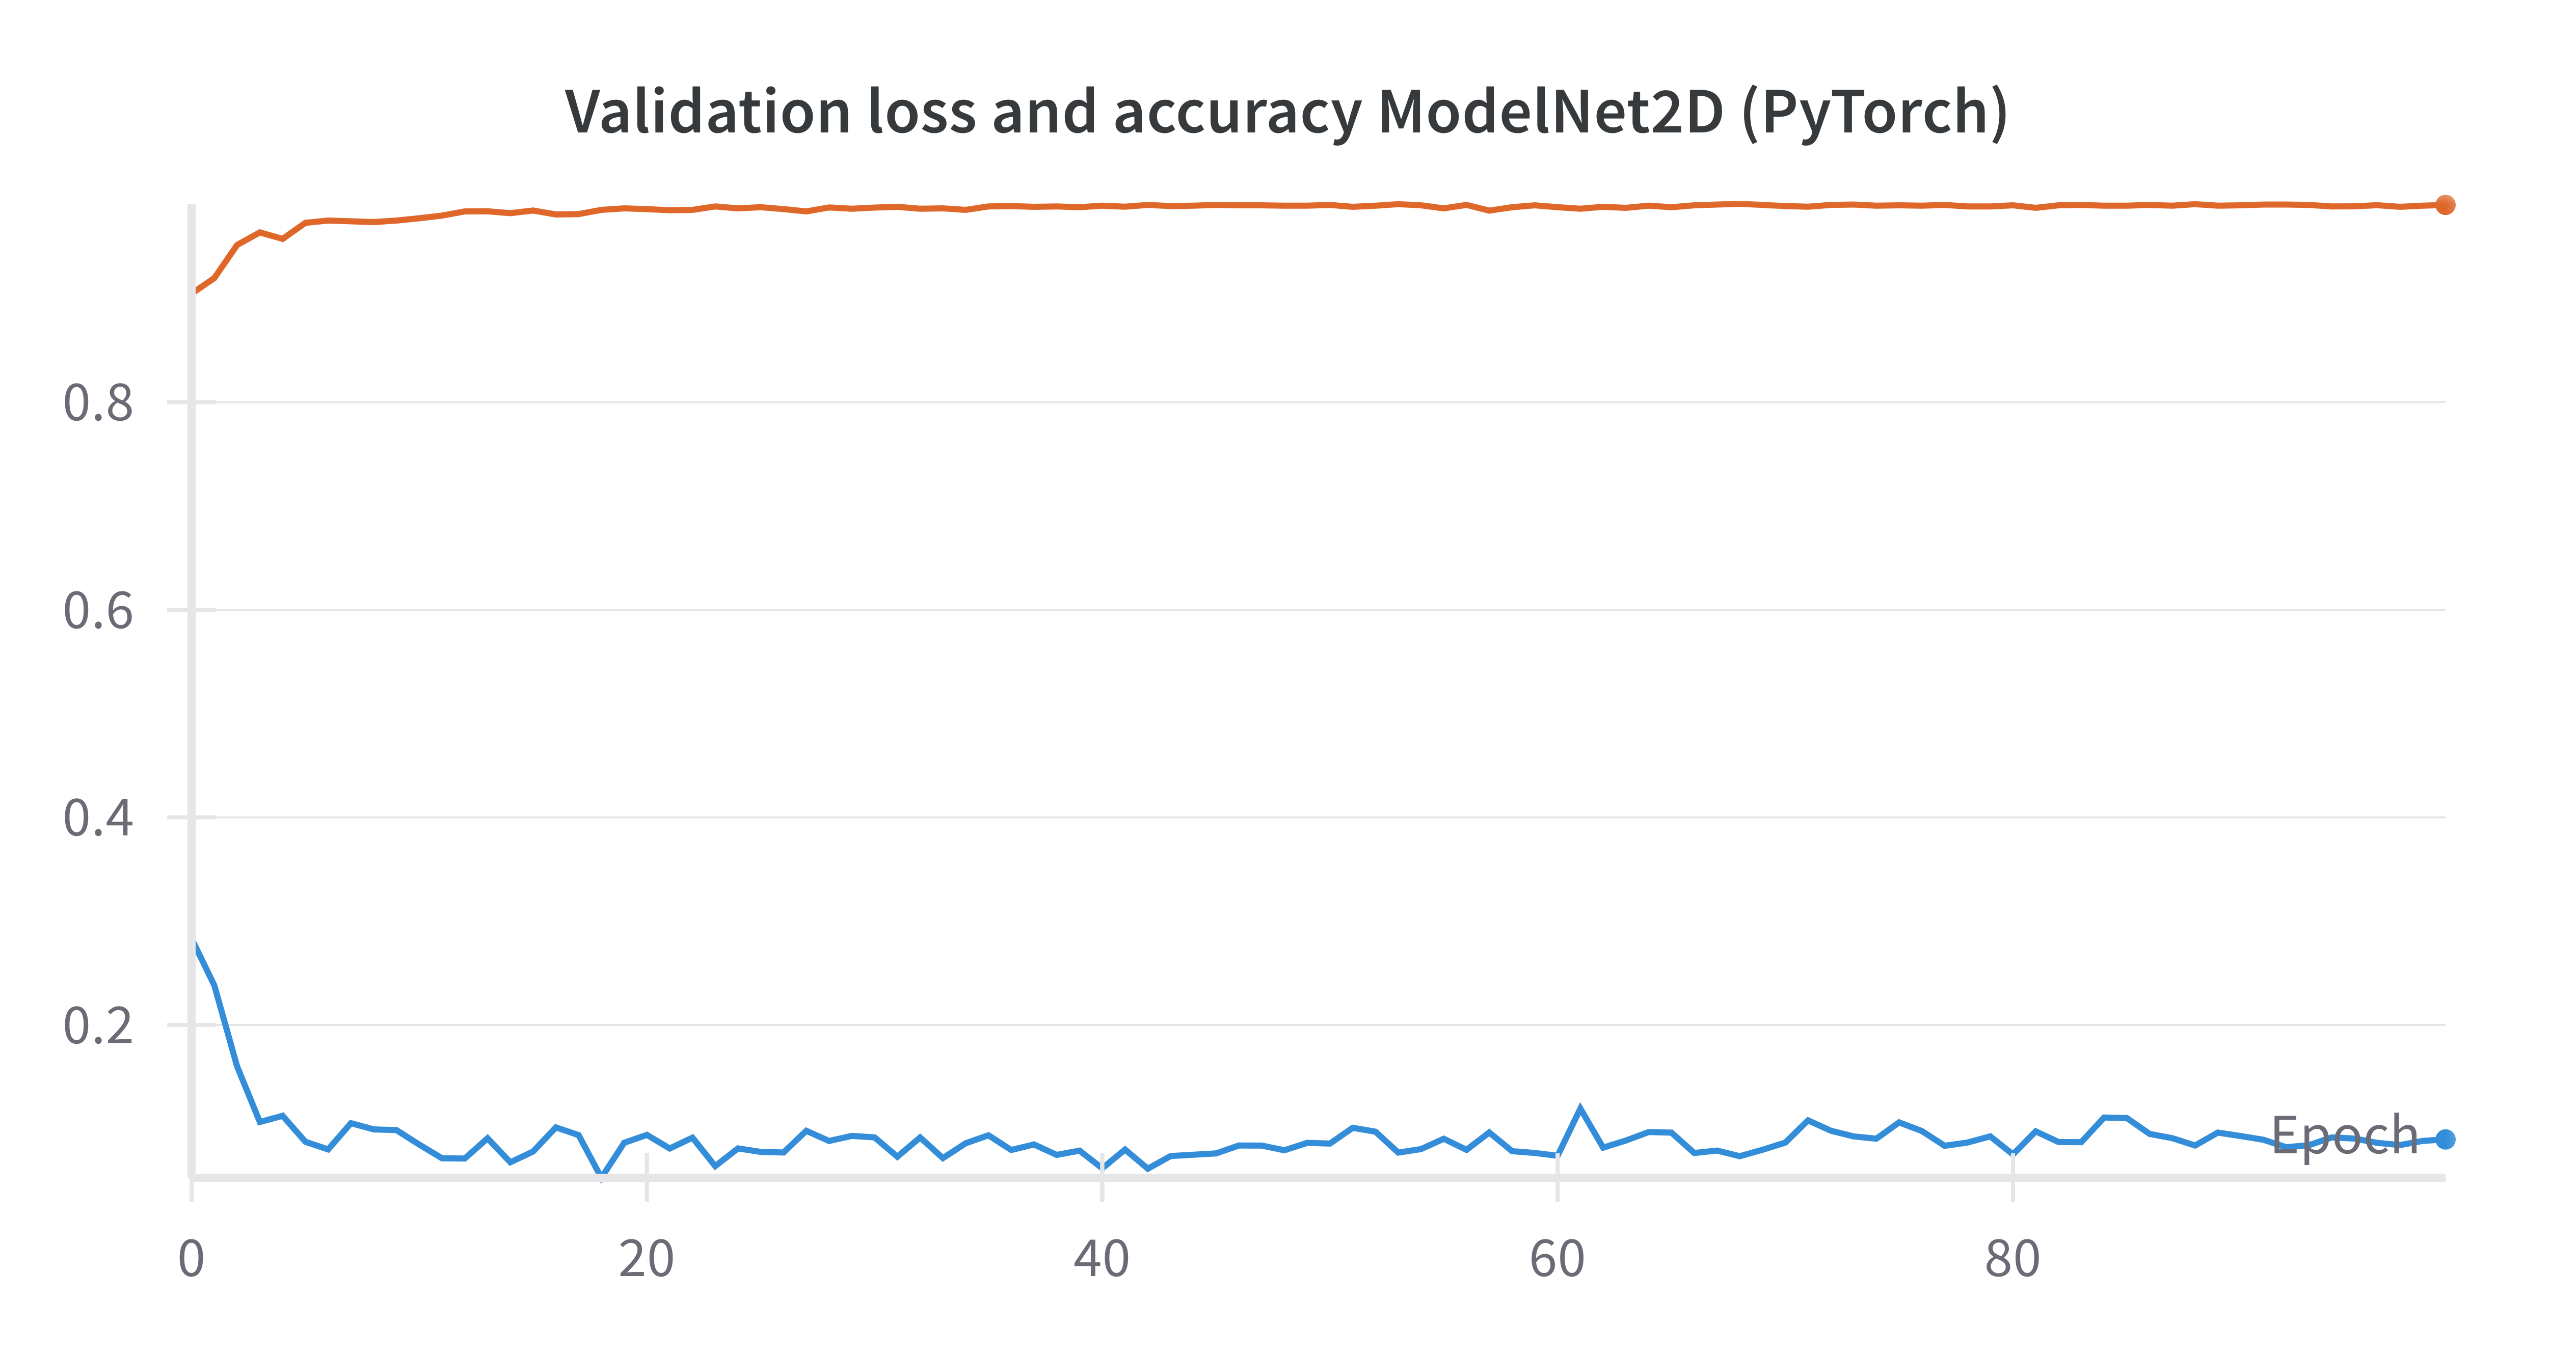
\includegraphics[width=1\linewidth]{modelnet_val_loss_acc_mod_pt.png}
			\caption{Validation loss/accuracy}
			\label{fig:modelnet2d_val_loss_acc_mod_pt}
		\end{subcaptionblock}%
	}
	\caption{Metriche del dataset ModelNet2D  (con training set modificato)}
	\label{fig:modelnet2d_train_val_loss_acc_mod_pt}
\end{figure}

\subsection{RGB-D Object}

\subsubsection{Codice originale}
Questo dataset, come il precedente, non è composto da immagini binoculari: per simulare la vista umana, gli autori hanno utilizzato coppie di immagini con gradi di azimut successivi.
Questa volta, la divisione del dataset presente nel codice originale degli autori è in linea con quanto scritto nell'articolo:
\begin{foreigndisplaycquote}{english}[\S4.1]{neurips2019:cnn2}
	On the RGB-D Object dataset, images of different objects are taken from different viewpoints. So, we use images taken from one third of continuous viewpoints of each object as the training set and the remaining images as the test set. We further split one third of the training images having continuous viewpoints as the validation set.
\end{foreigndisplaycquote}
Con questa divisione si ottengono: 3024 coppie di immagine per il training set, 1512 per il validation set e 9274 per il test set.
Siamo molto lontani dalle 250.000 immagini a colori descritte nell'articolo, ma il dataset originale è molto grande e qui si usano solo 5 classi di oggetti su 51.
Questo modello ha un layer di dropout, ma continua a non essere presente ne la funzione di \textit{fit}, ne la configurazione dell'\textit{early stopping}.

Nell'articolo, gli autori hanno effettuato diversi tentativi per riuscire ad individuare la configurazione ottimale del numero di filtri da utilizzare nel modello.
Nel loro codice è presente solo la configurazione che ha ottenuto il miglior valore di \textit{accuracy}, ed è anche la stessa che verrà usata nel codice di questo progetto.

Una differenza tra quanto scritto nell'articolo e il modello del loro codice è il numero di parametri: per i dataset con le immagini in scala di grigio, il numero è coerente con quello rilevato all'interno del modello, cioè circa 341K parametri, mentre per questo dataset (l'unico con immagini a colori) l'articolo indica la presenza di circa 493K parametri, mentre con il numero di filtri della configurazione ottimale (12 24 40), il numero di parametri non supera i 348K.
\begin{table}[!ht]
	\centering
	\begin{tabular}[t]{|c|cc|}
		\hline
		& \textbf{Accuracy} & \textbf{Loss} \\
		\hline
		training set articolo& 0.745 & 3.438 \\
		training set maggiore& 0.896 & 0.281 \\
		articolo & \textbf{0.868} & - \\
		\hline
	\end{tabular}
	\caption{Test loss/accuracy RGB-D}
	\label{tab:rgbd_val_loss_acc_pt}
\end{table}

\subsubsection{Codice del progetto}
Utilizzando la suddivisione del dataset presente nell'articolo (training set: 3024, test set: 9274 e validation set: 1512), il risultato è quello nella prima riga della tabella~\ref{tab:rgbd_val_loss_acc_pt}, inferiore a quanto ottenuto dagli autori.
Con quella suddivisione possiamo osservare, in figura~\ref{fig:rgbd_train_val_loss_acc_original_pt}, la stessa curva anomala della validation loss, vista in precedenza con il dataset small NORB.
\begin{figure}[ht]
	\centerline{% center image to the page, not to text
		\begin{subcaptionblock}{0.6\textwidth}
			\centering
			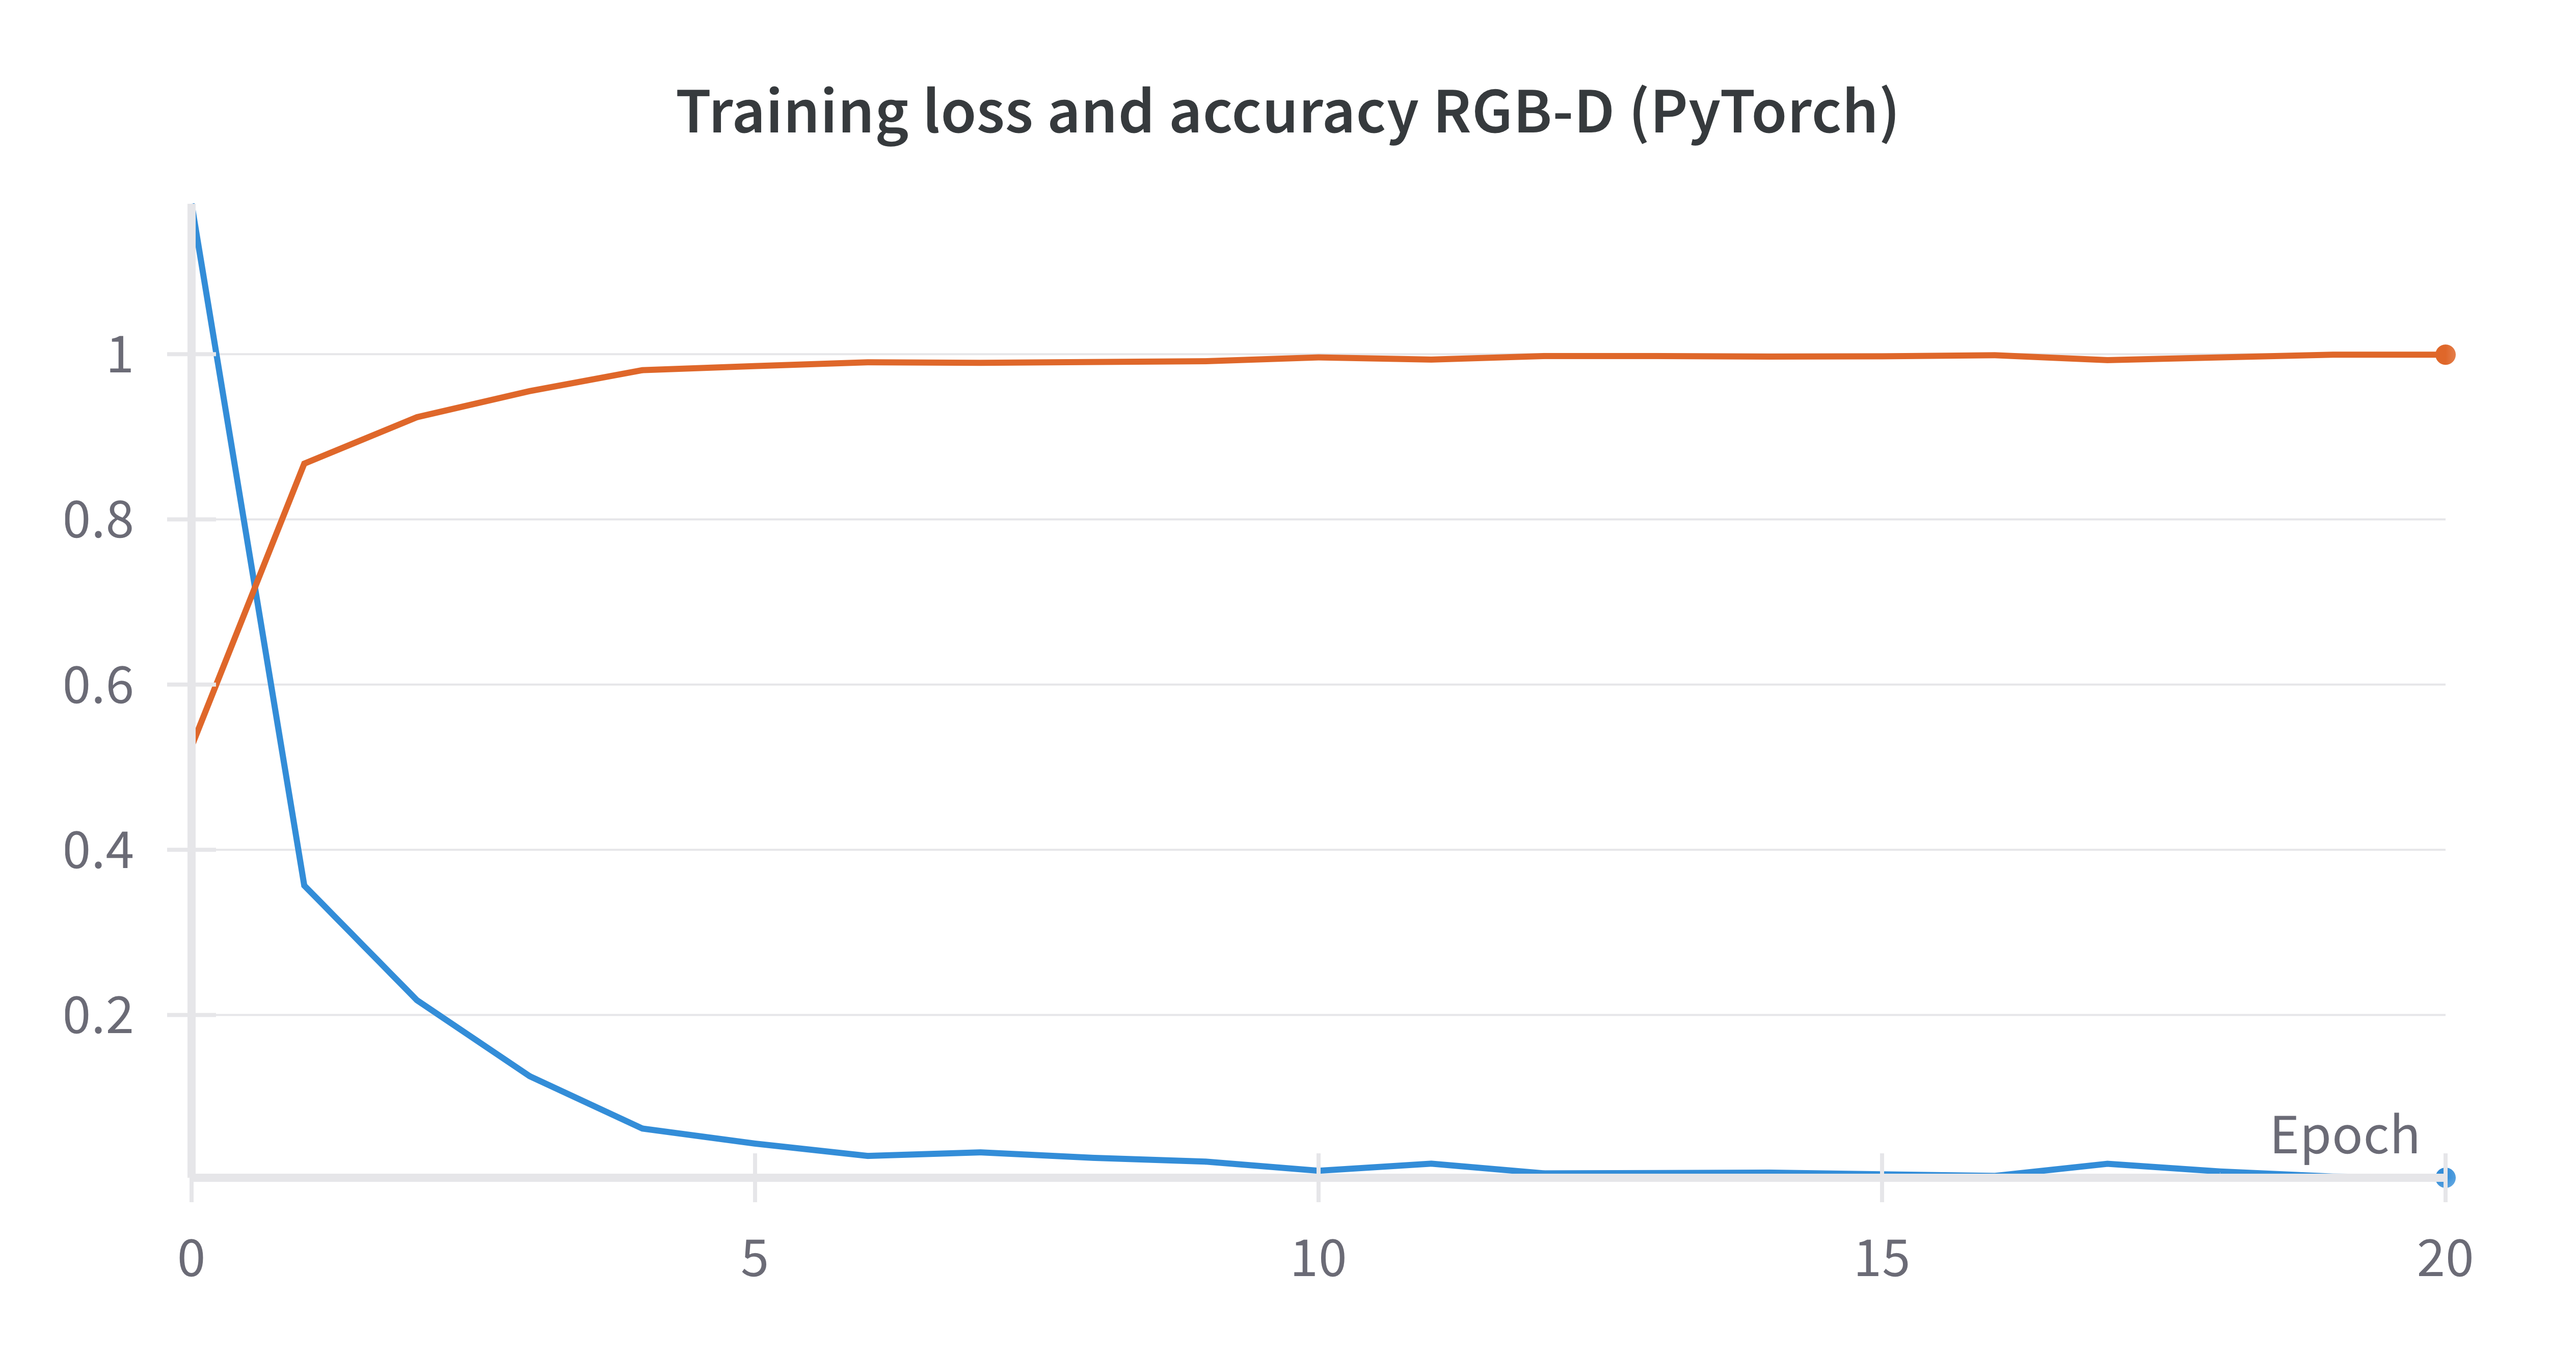
\includegraphics[width=1\linewidth]{rgbd_train_loss_acc_original_pt.png}
			\caption{Training  loss/accuracy}
			\label{fig:rgbd_train_loss_acc_original_pt}
		\end{subcaptionblock}%
		\begin{subcaptionblock}{0.6\textwidth}
			\centering
			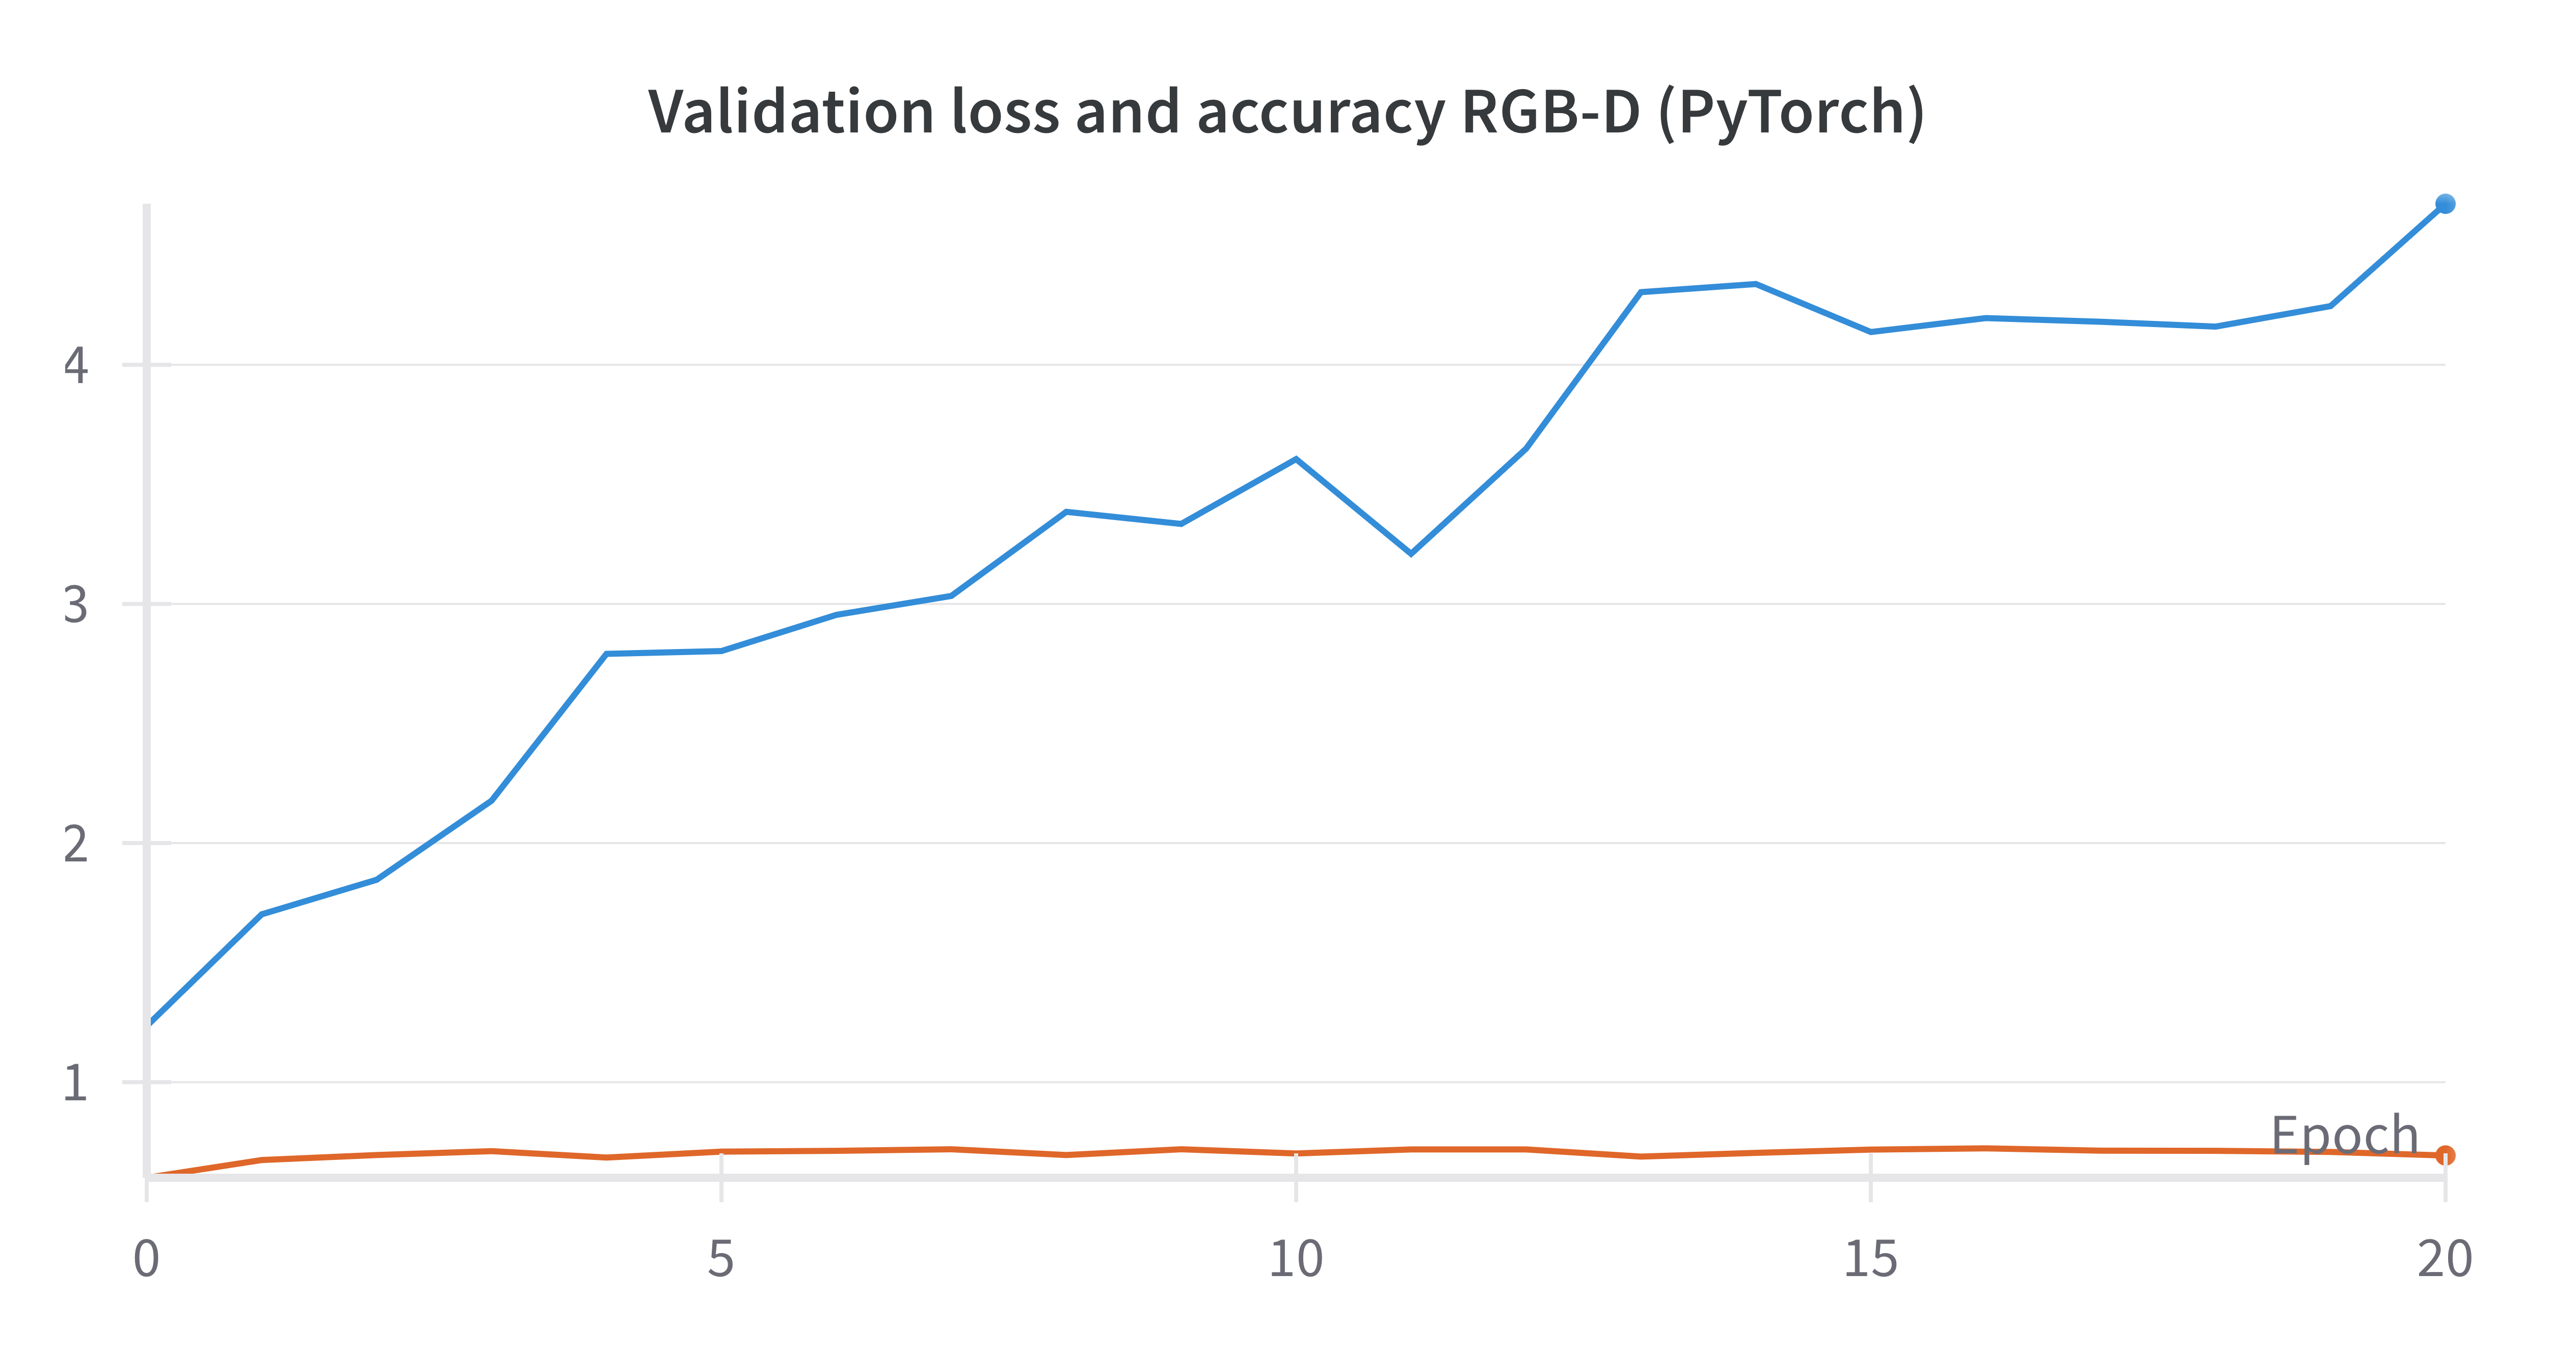
\includegraphics[width=1\linewidth]{rgbd_val_loss_acc_original_pt.png}
			\caption{Validation loss/accuracy}
			\label{fig:rgbd_val_loss_acc_original_pt}
		\end{subcaptionblock}%
	}
	\caption{Metriche del dataset RGB-D}
	\label{fig:rgbd_train_val_loss_acc_original_pt}
\end{figure}

\noindent Modificando il codice del progetto, aumentando i dati del training set a 9274 e riducendo quelli del test set a 3024, il modello sembra funzionare meglio, come possiamo vedere in figura~\ref{fig:modelnet2d_train_val_loss_acc_mod_pt}, anche se la curva della \textit{validation loss} non tende a diminuire: probabilmente servirebbero più immagini all'interno del training set.
I risultati ottenuti sono quelli presenti nella seconda riga della tabella~\ref{tab:rgbd_val_loss_acc_pt}.

\begin{figure}[ht]
	\centerline{% center image to the page, not to text
		\begin{subcaptionblock}{0.6\textwidth}
			\centering
			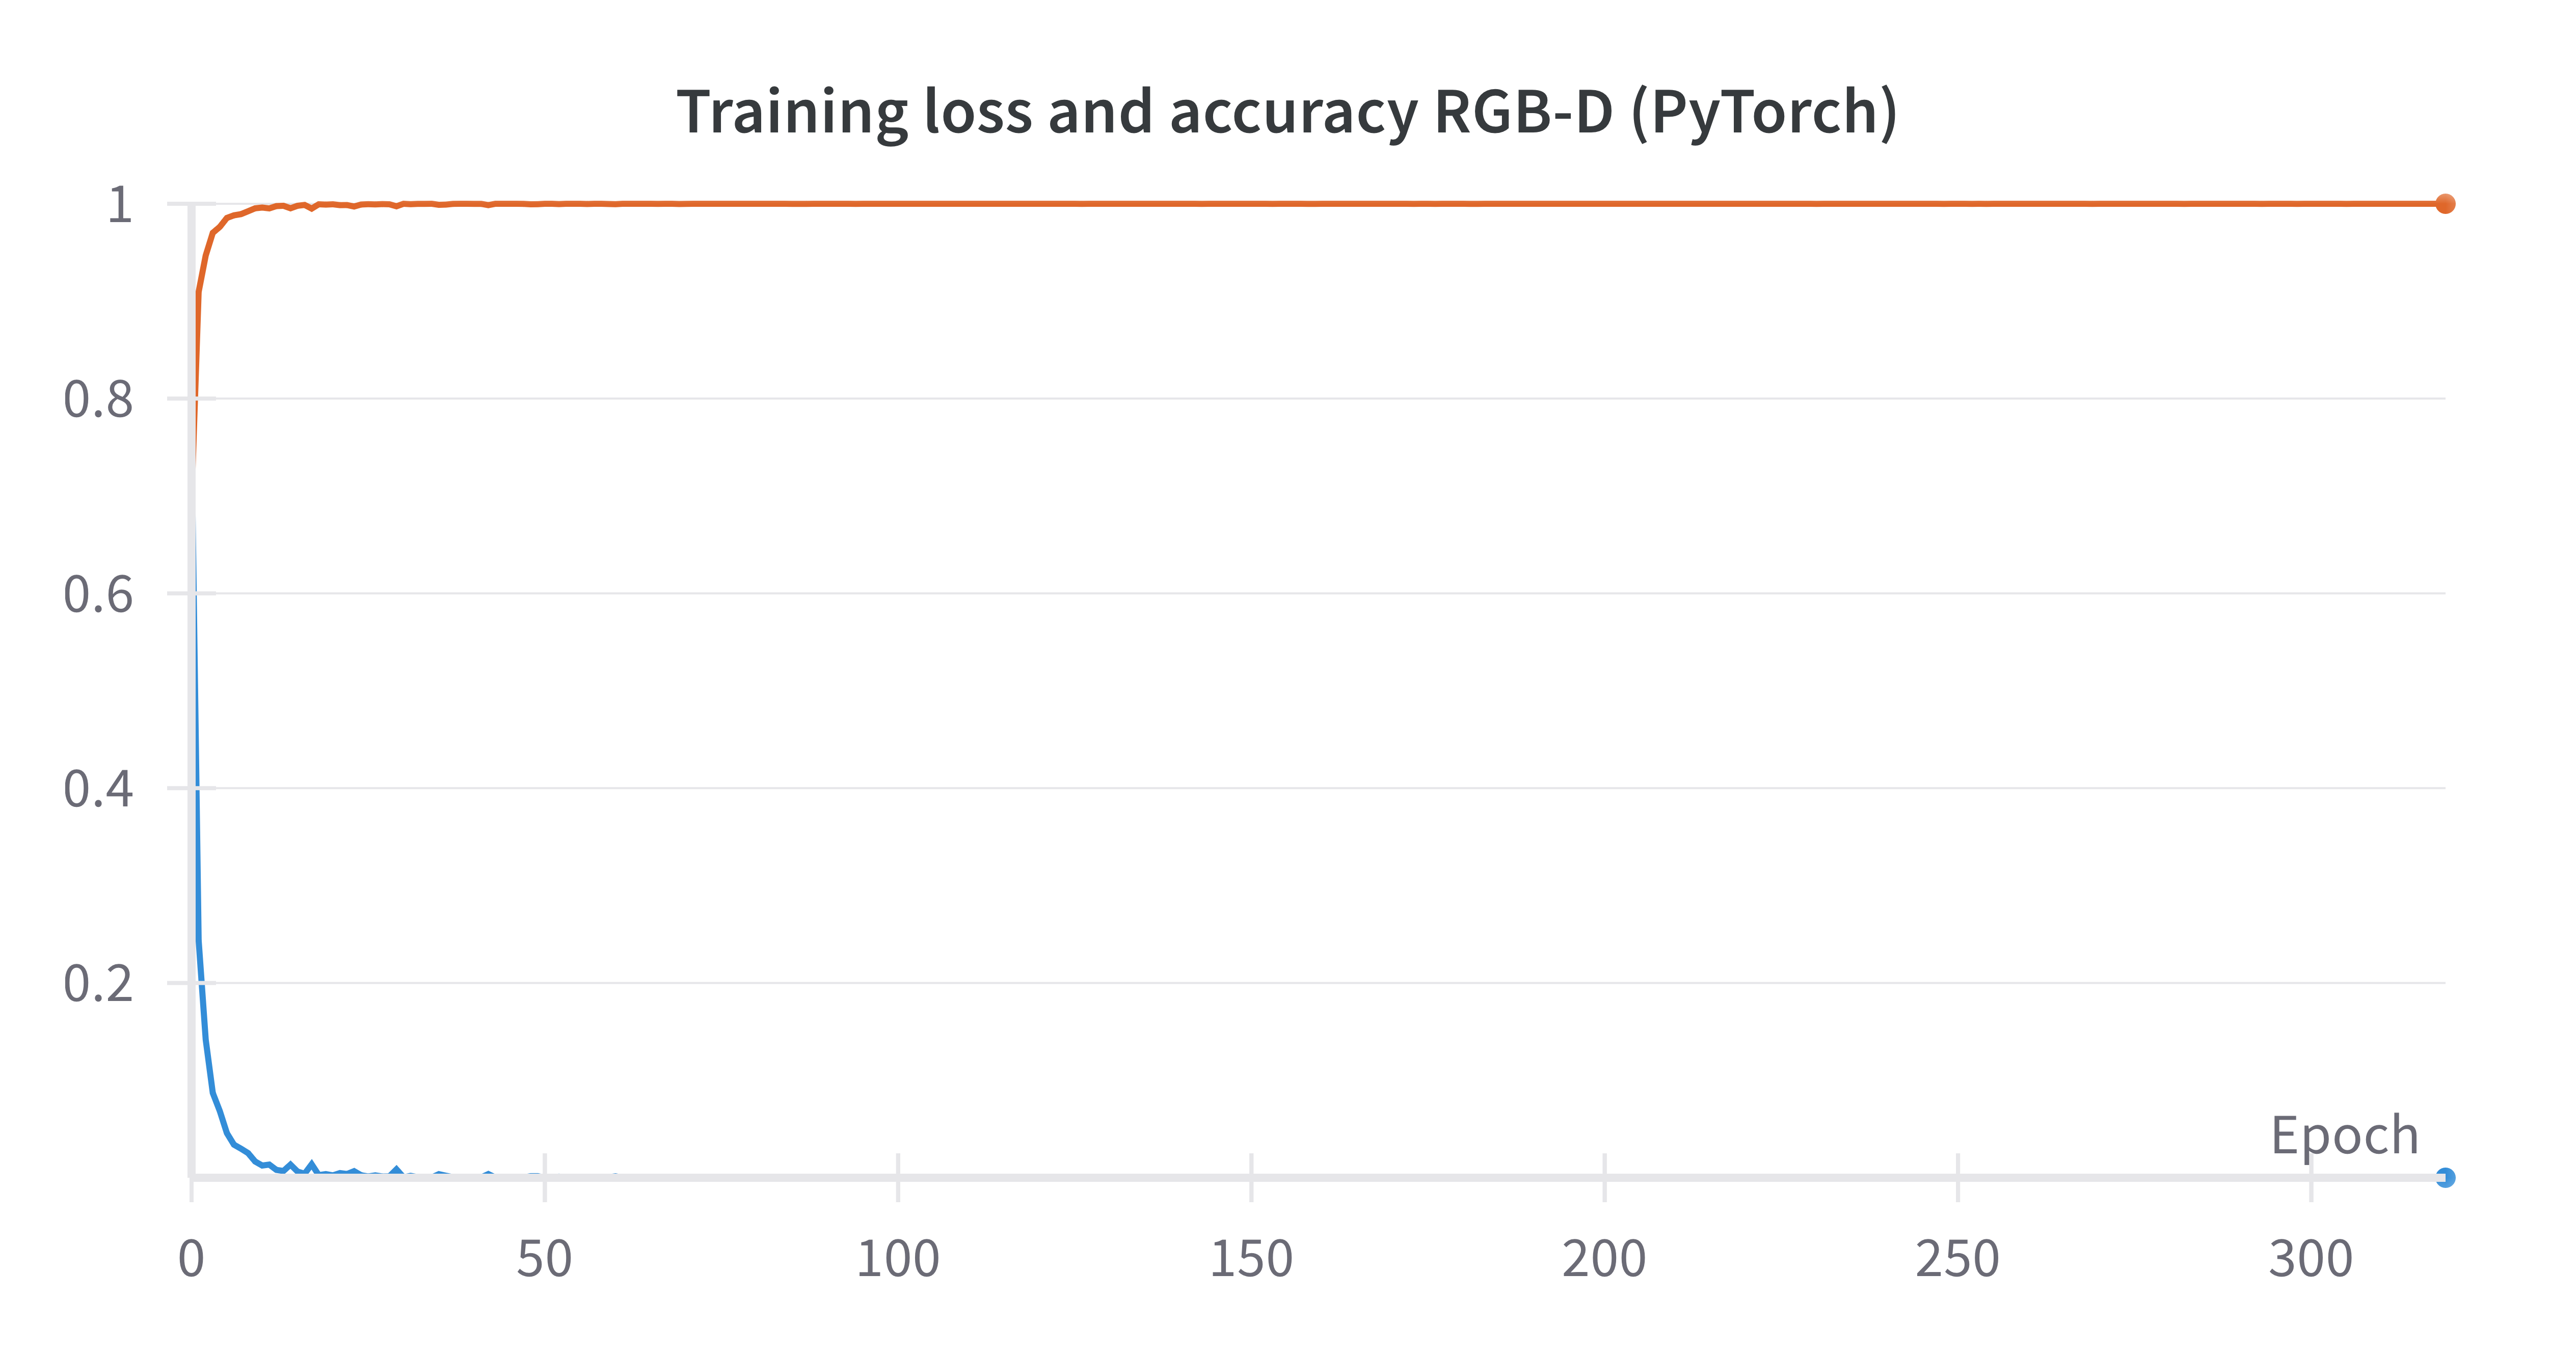
\includegraphics[width=1\linewidth]{rgbd_train_loss_acc_mod_pt.png}
			\caption{Training  loss/accuracy}
			\label{fig:rgbd_train_loss_acc_mod_pt}
		\end{subcaptionblock}%
		\begin{subcaptionblock}{0.6\textwidth}
			\centering
			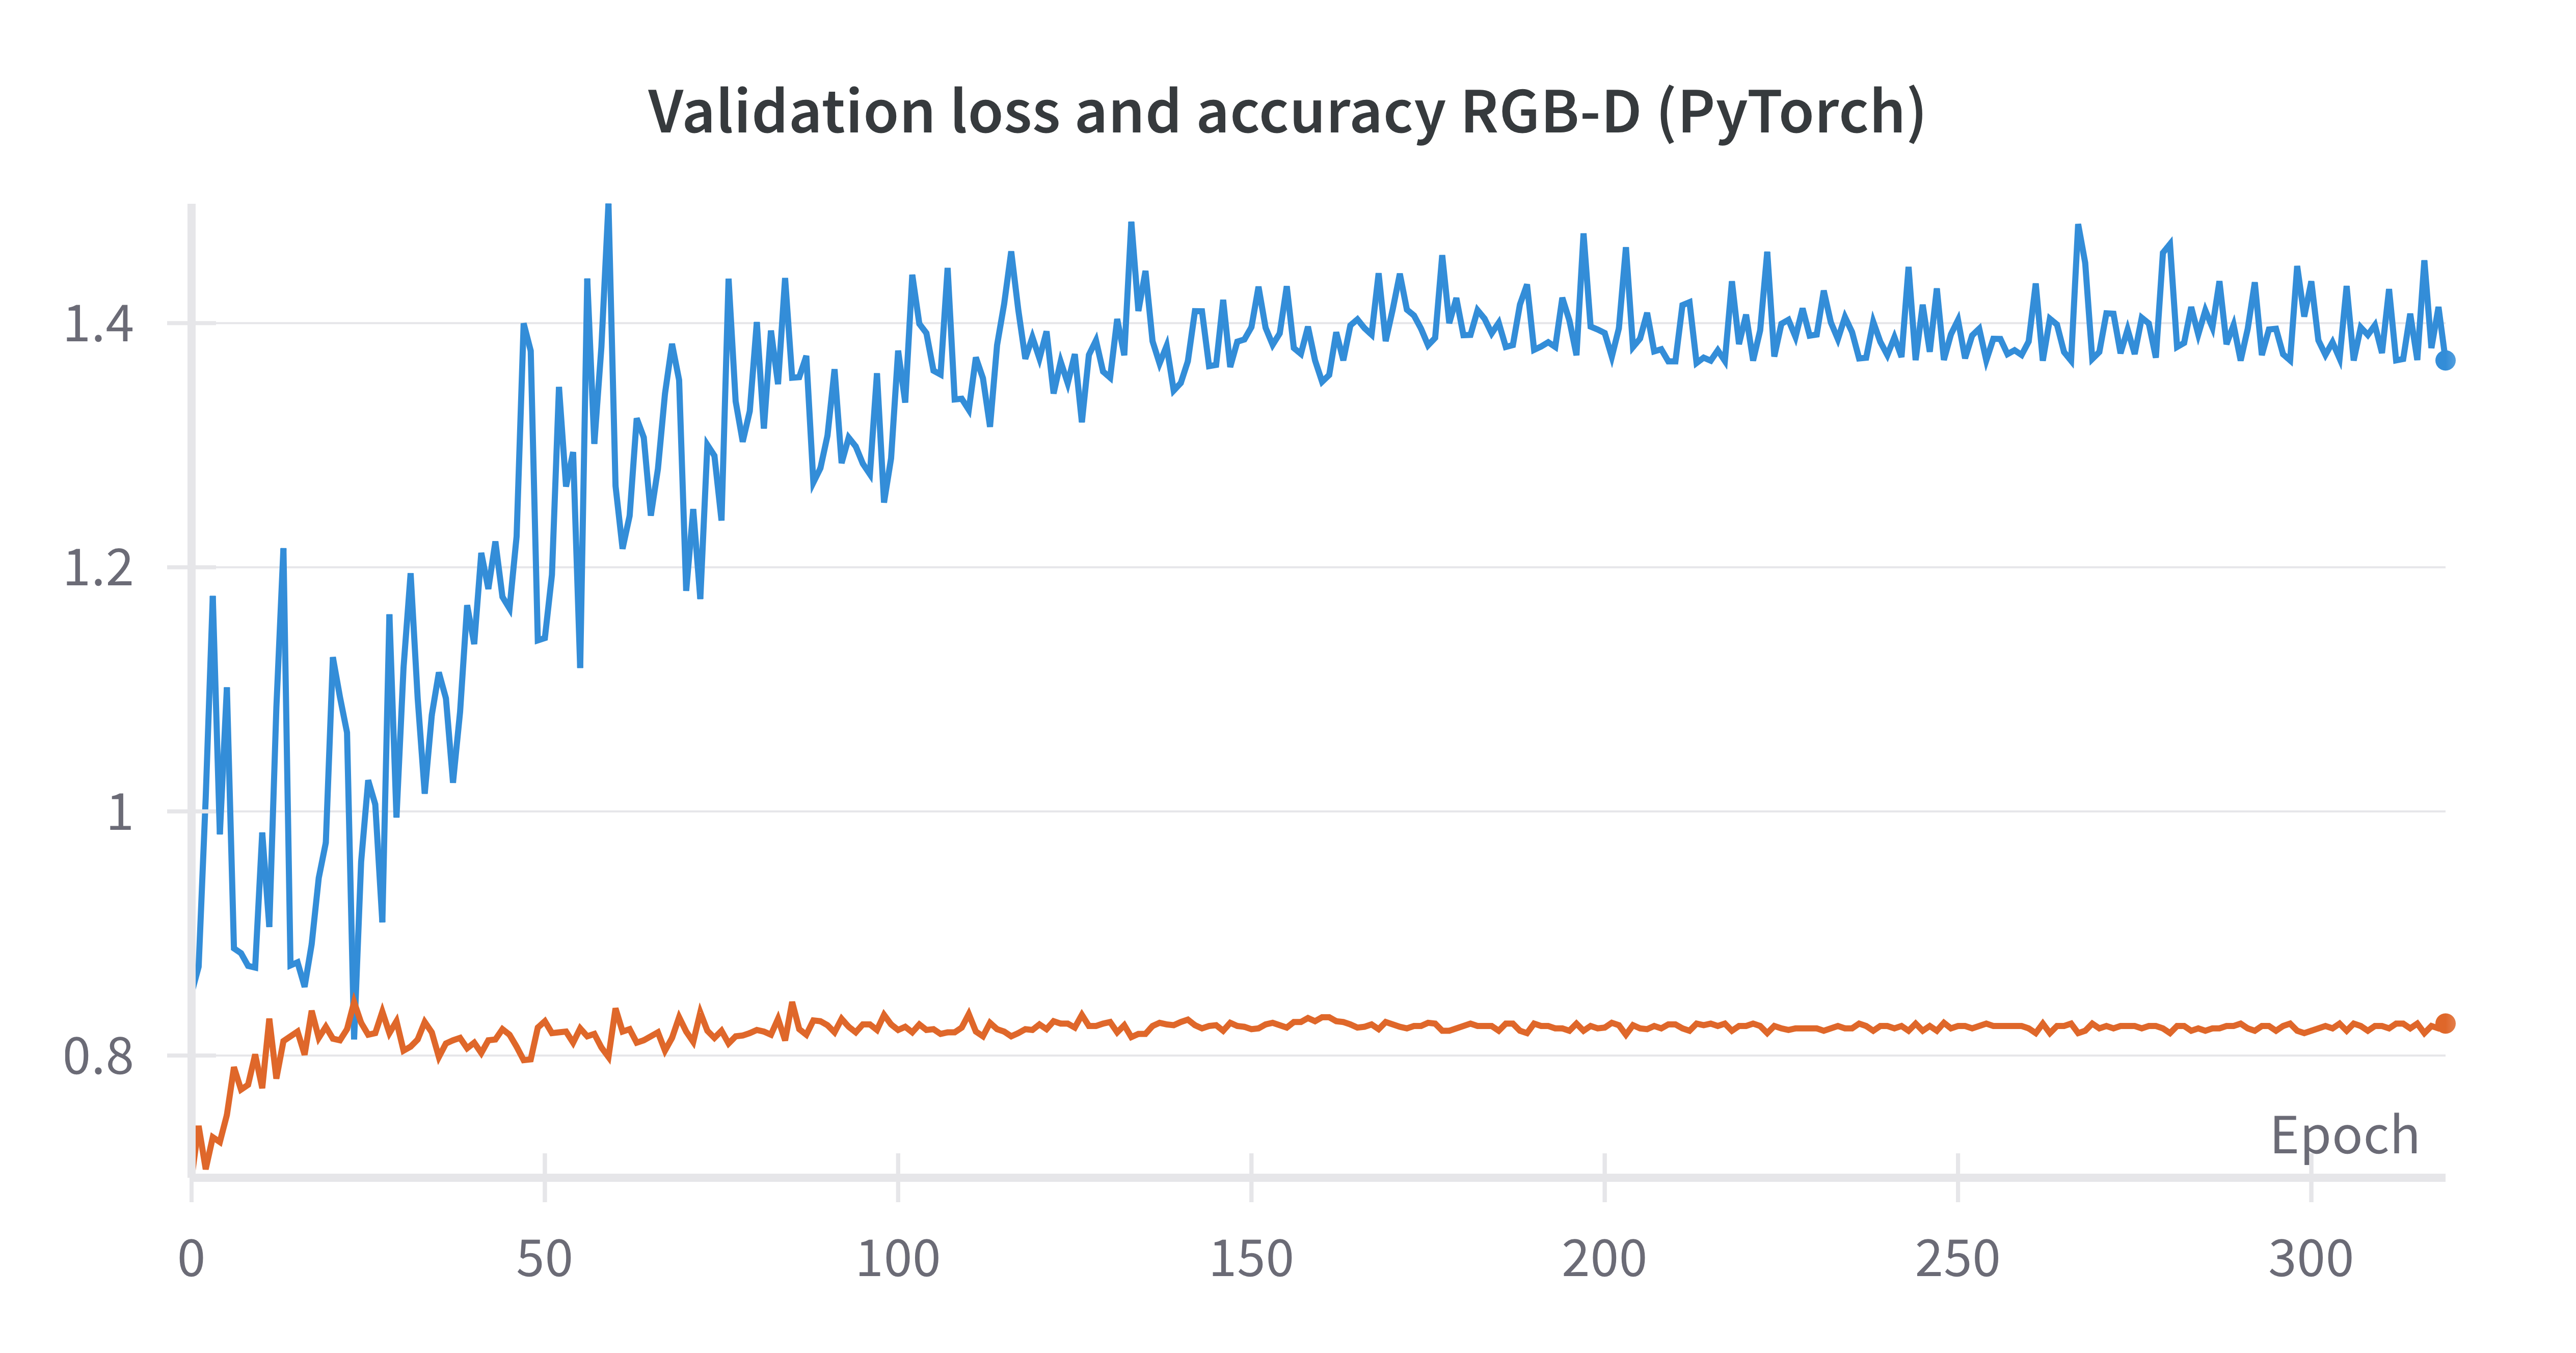
\includegraphics[width=1\linewidth]{rgbd_val_loss_acc_mod_pt.png}
			\caption{Validation loss/accuracy}
			\label{fig:rgbd_val_loss_acc_mod_pt}
		\end{subcaptionblock}%
	}
	\caption{Metriche del dataset RGB-D (con training set modificato)}
	\label{fig:rgbd_train_val_loss_acc_mod_pt}
\end{figure}

\newpage
\section{Risultati e commenti}
Lo scopo di questo progetto era quello di replicare i risultati principali presentati nell'articolo originale, senza utilizzare il codice rilasciato dagli autori, leggendo solo l'articolo e i materiali supplementari.
Purtroppo, come abbiamo visto in precedenza, all'interno dell'articolo mancano alcune informazioni necessarie per realizzare il modello: non è presente la descrizione del classificatore (figura~\ref{fig:cnn2_model}) e nemmeno la configurazione della procedura di \textit{early stopping}.
Fortunatamente, per quanto riguarda il classificatore, la struttura è stata ricavata dal codice sorgente messo a disposizione da parte degli autori, mentre non è stato possibile recuperare nessuna informazione riguardo l'\textit{early stopping}.

Per quanto riguarda il confronto tra i risultati presentati nell'articolo e quelli ottenuti con il codice realizzato per il progetto, non sempre i valori erano in linea: senza modifiche al numero di immagini utilizzate per addestrare il modello, i risultati erano sempre inferiori rispetto a quelli dell'articolo.
Anche le informazioni sul numero dei parametri e sui tempi di addestramento del modello, non hanno trovato riscontro usando il codice scritto per il progetto.
Per quanto riguarda i tempi di addestramento bisogna dire, però, che l'hardware usato durante il progetto, in particolare la GPU, era migliore rispetto a quello usato dagli autori.
Sono emerse, inoltre, varie discrepanze tra le informazioni dell'articolo e il codice degli sviluppatori: per i primi due dataset, la suddivisione tra training, validation e test set era diversa da quanto indicato nell'articolo e non era presente il layer di dropout nella configurazione del modello.
Questo ha reso impossibile replicare i risultati dell'articolo anche con il codice messo a disposizione dagli autori.

\printbibliography[heading=bibintoc] %Prints bibliography

\end{document}
